%%%%%%%%%%%%%%%%%%%%%%%%%%%%%%%%%%%%%%%%%
% The Legrand Orange Book
% LaTeX Template
% Version 1.4 (12/4/14)
%
% This template has been downloaded from:
% http://www.LaTeXTemplates.com
%
% Original author:
% Mathias Legrand (legrand.mathias@gmail.com)
%
% License:
% CC BY-NC-SA 3.0 (http://creativecommons.org/licenses/by-nc-sa/3.0/)
%
% Compiling this template:
% This template uses biber for its bibliography and makeindex for its index.
% When you first open the template, compile it from the command line with the 
% commands below to make sure your LaTeX distribution is configured correctly:
%
% 1) pdflatex main
% 2) makeindex main.idx -s StyleInd.ist
% 3) biber main
% 4) pdflatex main x 2
%
% After this, when you wish to update the bibliography/index use the appropriate
% command above and make sure to compile with pdflatex several times 
% afterwards to propagate your changes to the document.
%
% This template also uses a number of packages which may need to be
% updated to the newest versions for the template to compile. It is strongly
% recommended you update your LaTeX distribution if you have any
% compilation errors.
%
% Important note:
% Chapter heading images should have a 2:1 width:height ratio,
% e.g. 920px width and 460px height.
%
%%%%%%%%%%%%%%%%%%%%%%%%%%%%%%%%%%%%%%%%%

%----------------------------------------------------------------------------------------
%	PACKAGES AND OTHER DOCUMENT CONFIGURATIONS
%----------------------------------------------------------------------------------------

\documentclass[12pt,fleqn]{book} % Default font size and left-justified equations

\usepackage[top=3cm,bottom=3cm,left=3.2cm,right=3.2cm,headsep=10pt,a4paper]{geometry} % Page margins

\usepackage{xcolor} % Required for specifying colors by name
% \definecolor{ocre}{RGB}{243,102,25} % Define the orange color used for highlighting throughout the book
\definecolor{ocre}{RGB}{25,163,255} % Define the blue color used for highlighting throughout the book

% Font Settings
\usepackage{avant} % Use the Avantgarde font for headings
%\usepackage{times} % Use the Times font for headings
\usepackage{mathptmx} % Use the Adobe Times Roman as the default text font together with math symbols from the Sym­bol, Chancery and Com­puter Modern fonts

\usepackage{microtype} % Slightly tweak font spacing for aesthetics
\usepackage[utf8]{inputenc} % Required for including letters with accents
\usepackage[T1]{fontenc} % Use 8-bit encoding that has 256 glyphs

% Bibliography
% \usepackage[style=alphabetic,sorting=nyt,sortcites=true,autopunct=true,babel=hyphen,hyperref=true,abbreviate=false,backref=true,backend=biber]{biblatex}
\usepackage[]{biblatex}
\addbibresource{bibliography.bib} % BibTeX bibliography file
\defbibheading{bibempty}{}

% Index
\usepackage{calc} % For simpler calculation - used for spacing the index letter headings correctly
\usepackage{makeidx} % Required to make an index


\usepackage{algorithm}
\usepackage[noend]{algpseudocode}
\usepackage{graphicx}
\usepackage{subfigure}
\usepackage{multicol}


\renewcommand{\algorithmicrequire}{\textbf{Input:}}
\renewcommand{\algorithmicensure}{\textbf{Output:}}

\makeindex % Tells LaTeX to create the files required for indexing

%----------------------------------------------------------------------------------------

%----------------------------------------------------------------------------------------
%	VARIOUS REQUIRED PACKAGES
%----------------------------------------------------------------------------------------

\usepackage{titlesec} % Allows customization of titles

\usepackage{graphicx} % Required for including pictures
\graphicspath{{Pictures/}} % Specifies the directory where pictures are stored

\usepackage{lipsum} % Inserts dummy text

\usepackage{tikz} % Required for drawing custom shapes

\usepackage[english]{babel} % English language/hyphenation

\usepackage{enumitem} % Customize lists
\setlist{nolistsep} % Reduce spacing between bullet points and numbered lists

\usepackage{booktabs} % Required for nicer horizontal rules in tables

\usepackage{eso-pic} % Required for specifying an image background in the title page

%----------------------------------------------------------------------------------------
%	MAIN TABLE OF CONTENTS
%----------------------------------------------------------------------------------------

\usepackage{titletoc} % Required for manipulating the table of contents

\contentsmargin{0cm} % Removes the default margin
% Chapter text styling
\titlecontents{chapter}[1.25cm] % Indentation
{\addvspace{15pt}\large\sffamily\bfseries} % Spacing and font options for chapters
{\color{ocre!60}\contentslabel[\Large\thecontentslabel]{1.25cm}\color{ocre}} % Chapter number
{}  
{\color{ocre!60}\normalsize\sffamily\bfseries\;\titlerule*[.5pc]{.}\;\thecontentspage} % Page number
% Section text styling
\titlecontents{section}[1.25cm] % Indentation
{\addvspace{5pt}\sffamily\bfseries} % Spacing and font options for sections
{\contentslabel[\thecontentslabel]{1.25cm}} % Section number
{}
{\sffamily\hfill\color{black}\thecontentspage} % Page number
[]
% Subsection text styling
\titlecontents{subsection}[1.25cm] % Indentation
{\addvspace{1pt}\sffamily\small} % Spacing and font options for subsections
{\contentslabel[\thecontentslabel]{1.25cm}} % Subsection number
{}
{\sffamily\;\titlerule*[.5pc]{.}\;\thecontentspage} % Page number
[] 

%----------------------------------------------------------------------------------------
%	MINI TABLE OF CONTENTS IN CHAPTER HEADS
%----------------------------------------------------------------------------------------

% Section text styling
\titlecontents{lsection}[0em] % Indendating
{\footnotesize\sffamily} % Font settings
{}
{}
{}

% Subsection text styling
\titlecontents{lsubsection}[.5em] % Indentation
{\normalfont\footnotesize\sffamily} % Font settings
{}
{}
{}
 
%----------------------------------------------------------------------------------------
%	PAGE HEADERS
%----------------------------------------------------------------------------------------

\usepackage{fancyhdr} % Required for header and footer configuration

\pagestyle{fancy}
\renewcommand{\chaptermark}[1]{\markboth{\sffamily\normalsize\bfseries\chaptername\ \thechapter.\ #1}{}} % Chapter text font settings
\renewcommand{\sectionmark}[1]{\markright{\sffamily\normalsize\thesection\hspace{5pt}#1}{}} % Section text font settings
\fancyhf{} \fancyhead[LE,RO]{\sffamily\normalsize\thepage} % Font setting for the page number in the header
\fancyhead[LO]{\rightmark} % Print the nearest section name on the left side of odd pages
\fancyhead[RE]{\leftmark} % Print the current chapter name on the right side of even pages
\renewcommand{\headrulewidth}{0.5pt} % Width of the rule under the header
\addtolength{\headheight}{2.5pt} % Increase the spacing around the header slightly
\renewcommand{\footrulewidth}{0pt} % Removes the rule in the footer
\fancypagestyle{plain}{\fancyhead{}\renewcommand{\headrulewidth}{0pt}} % Style for when a plain pagestyle is specified

% Removes the header from odd empty pages at the end of chapters
\makeatletter
\renewcommand{\cleardoublepage}{
\clearpage\ifodd\c@page\else
\hbox{}
\vspace*{\fill}
\thispagestyle{empty}
\newpage
\fi}

%----------------------------------------------------------------------------------------
%	THEOREM STYLES
%----------------------------------------------------------------------------------------

\usepackage{amsmath,amsfonts,amssymb,amsthm} % For math equations, theorems, symbols, etc

\newcommand{\intoo}[2]{\mathopen{]}#1\,;#2\mathclose{[}}
\newcommand{\ud}{\mathop{\mathrm{{}d}}\mathopen{}}
\newcommand{\intff}[2]{\mathopen{[}#1\,;#2\mathclose{]}}
\newtheorem{notation}{Notation}[chapter]

%%%%%%%%%%%%%%%%%%%%%%%%%%%%%%%%%%%%%%%%%%%%%%%%%%%%%%%%%%%%%%%%%%%%%%%%%%%
%%%%%%%%%%%%%%%%%%%% dedicated to boxed/framed environements %%%%%%%%%%%%%%
%%%%%%%%%%%%%%%%%%%%%%%%%%%%%%%%%%%%%%%%%%%%%%%%%%%%%%%%%%%%%%%%%%%%%%%%%%%
\newtheoremstyle{ocrenumbox}% % Theorem style name
{0pt}% Space above
{0pt}% Space below
{\normalfont}% % Body font
{}% Indent amount
{\small\bf\sffamily\color{ocre}}% % Theorem head font
{\;}% Punctuation after theorem head
{0.25em}% Space after theorem head
{\small\sffamily\color{ocre}\thmname{#1}\nobreakspace\thmnumber{\@ifnotempty{#1}{}\@upn{#2}}% Theorem text (e.g. Theorem 2.1)
\thmnote{\nobreakspace\the\thm@notefont\sffamily\bfseries\color{black}---\nobreakspace#3.}} % Optional theorem note
\renewcommand{\qedsymbol}{$\blacksquare$}% Optional qed square

\newtheoremstyle{blacknumex}% Theorem style name
{5pt}% Space above
{5pt}% Space below
{\normalfont}% Body font
{} % Indent amount
{\small\bf\sffamily}% Theorem head font
{\;}% Punctuation after theorem head
{0.25em}% Space after theorem head
{\small\sffamily{\tiny\ensuremath{\blacksquare}}\nobreakspace\thmname{#1}\nobreakspace\thmnumber{\@ifnotempty{#1}{}\@upn{#2}}% Theorem text (e.g. Theorem 2.1)
\thmnote{\nobreakspace\the\thm@notefont\sffamily\bfseries---\nobreakspace#3.}}% Optional theorem note

\newtheoremstyle{blacknumbox} % Theorem style name
{0pt}% Space above
{0pt}% Space below
{\normalfont}% Body font
{}% Indent amount
{\small\bf\sffamily}% Theorem head font
{\;}% Punctuation after theorem head
{0.25em}% Space after theorem head
{\small\sffamily\thmname{#1}\nobreakspace\thmnumber{\@ifnotempty{#1}{}\@upn{#2}}% Theorem text (e.g. Theorem 2.1)
\thmnote{\nobreakspace\the\thm@notefont\sffamily\bfseries---\nobreakspace#3.}}% Optional theorem note

%%%%%%%%%%%%%%%%%%%%%%%%%%%%%%%%%%%%%%%%%%%%%%%%%%%%%%%%%%%%%%%%%%%%%%%%%%%
%%%%%%%%%%%%% dedicated to non-boxed/non-framed environements %%%%%%%%%%%%%
%%%%%%%%%%%%%%%%%%%%%%%%%%%%%%%%%%%%%%%%%%%%%%%%%%%%%%%%%%%%%%%%%%%%%%%%%%%
\newtheoremstyle{ocrenum}% % Theorem style name
{5pt}% Space above
{5pt}% Space below
{\normalfont}% % Body font
{}% Indent amount
{\small\bf\sffamily\color{ocre}}% % Theorem head font
{\;}% Punctuation after theorem head
{0.25em}% Space after theorem head
{\small\sffamily\color{ocre}\thmname{#1}\nobreakspace\thmnumber{\@ifnotempty{#1}{}\@upn{#2}}% Theorem text (e.g. Theorem 2.1)
\thmnote{\nobreakspace\the\thm@notefont\sffamily\bfseries\color{black}---\nobreakspace#3.}} % Optional theorem note
\renewcommand{\qedsymbol}{$\blacksquare$}% Optional qed square
\makeatother

% Defines the theorem text style for each type of theorem to one of the three styles above
\newcounter{dummy} 
\numberwithin{dummy}{section}
\theoremstyle{ocrenumbox}
\newtheorem{theoremeT}[dummy]{Theorem}
\newtheorem{problem}{Problem}[chapter]
\newtheorem{exerciseT}{Exercise}[chapter]
\theoremstyle{blacknumex}
\newtheorem{exampleT}{Example}[chapter]
\theoremstyle{blacknumbox}
\newtheorem{vocabulary}{Vocabulary}[chapter]
\newtheorem{definitionT}{Definition}[section]
\newtheorem{corollaryT}[dummy]{Corollary}
\theoremstyle{ocrenum}
\newtheorem{proposition}[dummy]{Proposition}

%----------------------------------------------------------------------------------------
%	DEFINITION OF COLORED BOXES
%----------------------------------------------------------------------------------------

\RequirePackage[framemethod=default]{mdframed} % Required for creating the theorem, definition, exercise and corollary boxes

% Theorem box
\newmdenv[skipabove=7pt,
skipbelow=7pt,
backgroundcolor=black!5,
linecolor=ocre,
innerleftmargin=5pt,
innerrightmargin=5pt,
innertopmargin=5pt,
leftmargin=0cm,
rightmargin=0cm,
innerbottommargin=5pt]{tBox}

% Exercise box	  
\newmdenv[skipabove=7pt,
skipbelow=7pt,
rightline=false,
leftline=true,
topline=false,
bottomline=false,
backgroundcolor=ocre!10,
linecolor=ocre,
innerleftmargin=5pt,
innerrightmargin=5pt,
innertopmargin=5pt,
innerbottommargin=5pt,
leftmargin=0cm,
rightmargin=0cm,
linewidth=4pt]{eBox}	

% Definition box
\newmdenv[skipabove=7pt,
skipbelow=7pt,
rightline=false,
leftline=true,
topline=false,
bottomline=false,
linecolor=ocre,
innerleftmargin=5pt,
innerrightmargin=5pt,
innertopmargin=0pt,
leftmargin=0cm,
rightmargin=0cm,
linewidth=4pt,
innerbottommargin=0pt]{dBox}	

% Corollary box
\newmdenv[skipabove=7pt,
skipbelow=7pt,
rightline=false,
leftline=true,
topline=false,
bottomline=false,
linecolor=gray,
backgroundcolor=black!5,
innerleftmargin=5pt,
innerrightmargin=5pt,
innertopmargin=5pt,
leftmargin=0cm,
rightmargin=0cm,
linewidth=4pt,
innerbottommargin=5pt]{cBox}

% Creates an environment for each type of theorem and assigns it a theorem text style from the "Theorem Styles" section above and a colored box from above
\newenvironment{theorem}{\begin{tBox}\begin{theoremeT}}{\end{theoremeT}\end{tBox}}
\newenvironment{exercise}{\begin{eBox}\begin{exerciseT}}{\hfill{\color{ocre}\tiny\ensuremath{\blacksquare}}\end{exerciseT}\end{eBox}}				  
\newenvironment{definition}{\begin{dBox}\begin{definitionT}}{\end{definitionT}\end{dBox}}	
\newenvironment{example}{\begin{exampleT}}{\hfill{\tiny\ensuremath{\blacksquare}}\end{exampleT}}		
\newenvironment{corollary}{\begin{cBox}\begin{corollaryT}}{\end{corollaryT}\end{cBox}}	

%----------------------------------------------------------------------------------------
%	REMARK ENVIRONMENT
%----------------------------------------------------------------------------------------

\newenvironment{remark}{\par\vspace{10pt}\small % Vertical white space above the remark and smaller font size
\begin{list}{}{
\leftmargin=35pt % Indentation on the left
\rightmargin=25pt}\item\ignorespaces % Indentation on the right
\makebox[-2.5pt]{\begin{tikzpicture}[overlay]
\node[draw=ocre!60,line width=1pt,circle,fill=ocre!25,font=\sffamily\bfseries,inner sep=2pt,outer sep=0pt] at (-15pt,0pt){\textcolor{ocre}{R}};\end{tikzpicture}} % Orange R in a circle
\advance\baselineskip -1pt}{\end{list}\vskip5pt} % Tighter line spacing and white space after remark


% modified remark envirnment to mark our implementation section in the book
\newenvironment{our}{ 
\begin{list}{}{
\leftmargin=0pt % Indentation on the left
\rightmargin=0pt}\item\ignorespaces % Indentation on the right
\makebox[-2.5pt]{\begin{tikzpicture}[overlay]
\node[draw=ocre!60,line width=1pt,circle,fill=ocre!25,font=\sffamily\bfseries,inner sep=2pt,outer sep=0pt] at (-15pt,0pt){\textcolor{ocre}{R}};\end{tikzpicture}} % R in a circle
\advance\baselineskip 0pt}{\end{list}\vskip5pt} % Tighter line spacing and white space after remark


%----------------------------------------------------------------------------------------
%	SECTION NUMBERING IN THE MARGIN
%----------------------------------------------------------------------------------------

\makeatletter
\renewcommand{\@seccntformat}[1]{\llap{\textcolor{ocre}{\csname the#1\endcsname}\hspace{1em}}}                    
\renewcommand{\section}{\@startsection{section}{1}{\z@}
{-4ex \@plus -1ex \@minus -.4ex}
{1ex \@plus.2ex }
{\normalfont\large\sffamily\bfseries}}
\renewcommand{\subsection}{\@startsection {subsection}{2}{\z@}
{-3ex \@plus -0.1ex \@minus -.4ex}
{0.5ex \@plus.2ex }
{\normalfont\sffamily\bfseries}}
\renewcommand{\subsubsection}{\@startsection {subsubsection}{3}{\z@}
{-2ex \@plus -0.1ex \@minus -.2ex}
{.2ex \@plus.2ex }
{\normalfont\small\sffamily\bfseries}}                        
\renewcommand\paragraph{\@startsection{paragraph}{4}{\z@}
{-2ex \@plus-.2ex \@minus .2ex}
{.1ex}
{\normalfont\small\sffamily\bfseries}}

%----------------------------------------------------------------------------------------
%	HYPERLINKS IN THE DOCUMENTS
%----------------------------------------------------------------------------------------

% For an unclear reason, the package should be loaded now and not later
\usepackage{hyperref}
\hypersetup{hidelinks,backref=true,pagebackref=true,hyperindex=true,colorlinks=false,breaklinks=true,urlcolor= ocre,bookmarks=true,bookmarksopen=false,pdftitle={Title},pdfauthor={Author}}

%----------------------------------------------------------------------------------------
%	CHAPTER HEADINGS
%----------------------------------------------------------------------------------------

% The set-up below should be (sadly) manually adapted to the overall margin page septup controlled by the geometry package loaded in the main.tex document. It is possible to implement below the dimensions used in the goemetry package (top,bottom,left,right)... TO BE DONE

\newcommand{\thechapterimage}{}
\newcommand{\chapterimage}[1]{\renewcommand{\thechapterimage}{#1}}

% Numbered chapters with mini tableofcontents
\def\thechapter{\arabic{chapter}}
\def\@makechapterhead#1{
\thispagestyle{empty}
{\centering \normalfont\sffamily
\ifnum \c@secnumdepth >\m@ne
\if@mainmatter
\startcontents
\begin{tikzpicture}[remember picture,overlay]
\node at (current page.north west)
{\begin{tikzpicture}[remember picture,overlay]
\node[anchor=north west,inner sep=0pt] at (0,0) {\includegraphics[width=\paperwidth]{\thechapterimage}};
%%%%%%%%%%%%%%%%%%%%%%%%%%%%%%%%%%%%%%%%%%%%%%%%%%%%%%%%%%%%%%%%%%%%%%%%%%%%%%%%%%%%%
% Commenting the 3 lines below removes the small contents box in the chapter heading
\fill[color=ocre!10!white,opacity=.6] (1cm,0) rectangle (8cm,-7cm);
\node[anchor=north west] at (1.1cm,.35cm) {\parbox[t][8cm][t]{6.5cm}{\huge\bfseries\flushleft \printcontents{l}{1}{\setcounter{tocdepth}{2}}}};
\draw[anchor=west] (5cm,-9cm) node [rounded corners=20pt,fill=ocre!10!white,text opacity=1,draw=ocre,draw opacity=1,line width=1.5pt,fill opacity=.6,inner sep=12pt]{\huge\sffamily\bfseries\textcolor{black}{\thechapter. #1\strut\makebox[22cm]{}}};
%%%%%%%%%%%%%%%%%%%%%%%%%%%%%%%%%%%%%%%%%%%%%%%%%%%%%%%%%%%%%%%%%%%%%%%%%%%%%%%%%%%%%
\end{tikzpicture}};
\end{tikzpicture}}
\par\vspace*{230\p@}
\fi
\fi}

% Unnumbered chapters without mini tableofcontents (could be added though) 
\def\@makeschapterhead#1{
\thispagestyle{empty}
{\centering \normalfont\sffamily
\ifnum \c@secnumdepth >\m@ne
\if@mainmatter
\begin{tikzpicture}[remember picture,overlay]
\node at (current page.north west)
{\begin{tikzpicture}[remember picture,overlay]
\node[anchor=north west,inner sep=0pt] at (0,0) {\includegraphics[width=\paperwidth]{\thechapterimage}};
\draw[anchor=west] (5cm,-9cm) node [rounded corners=20pt,fill=ocre!10!white,fill opacity=.6,inner sep=12pt,text opacity=1,draw=ocre,draw opacity=1,line width=1.5pt]{\huge\sffamily\bfseries\textcolor{black}{#1\strut\makebox[22cm]{}}};
\end{tikzpicture}};
\end{tikzpicture}}
\par\vspace*{230\p@}
\fi
\fi
}
\makeatother % Insert the commands.tex file which contains the majority of the structure behind the template

\begin{document}

%----------------------------------------------------------------------------------------
%	TITLE PAGE
%----------------------------------------------------------------------------------------

\begingroup
\thispagestyle{empty}
\AddToShipoutPicture*{\put(6,5){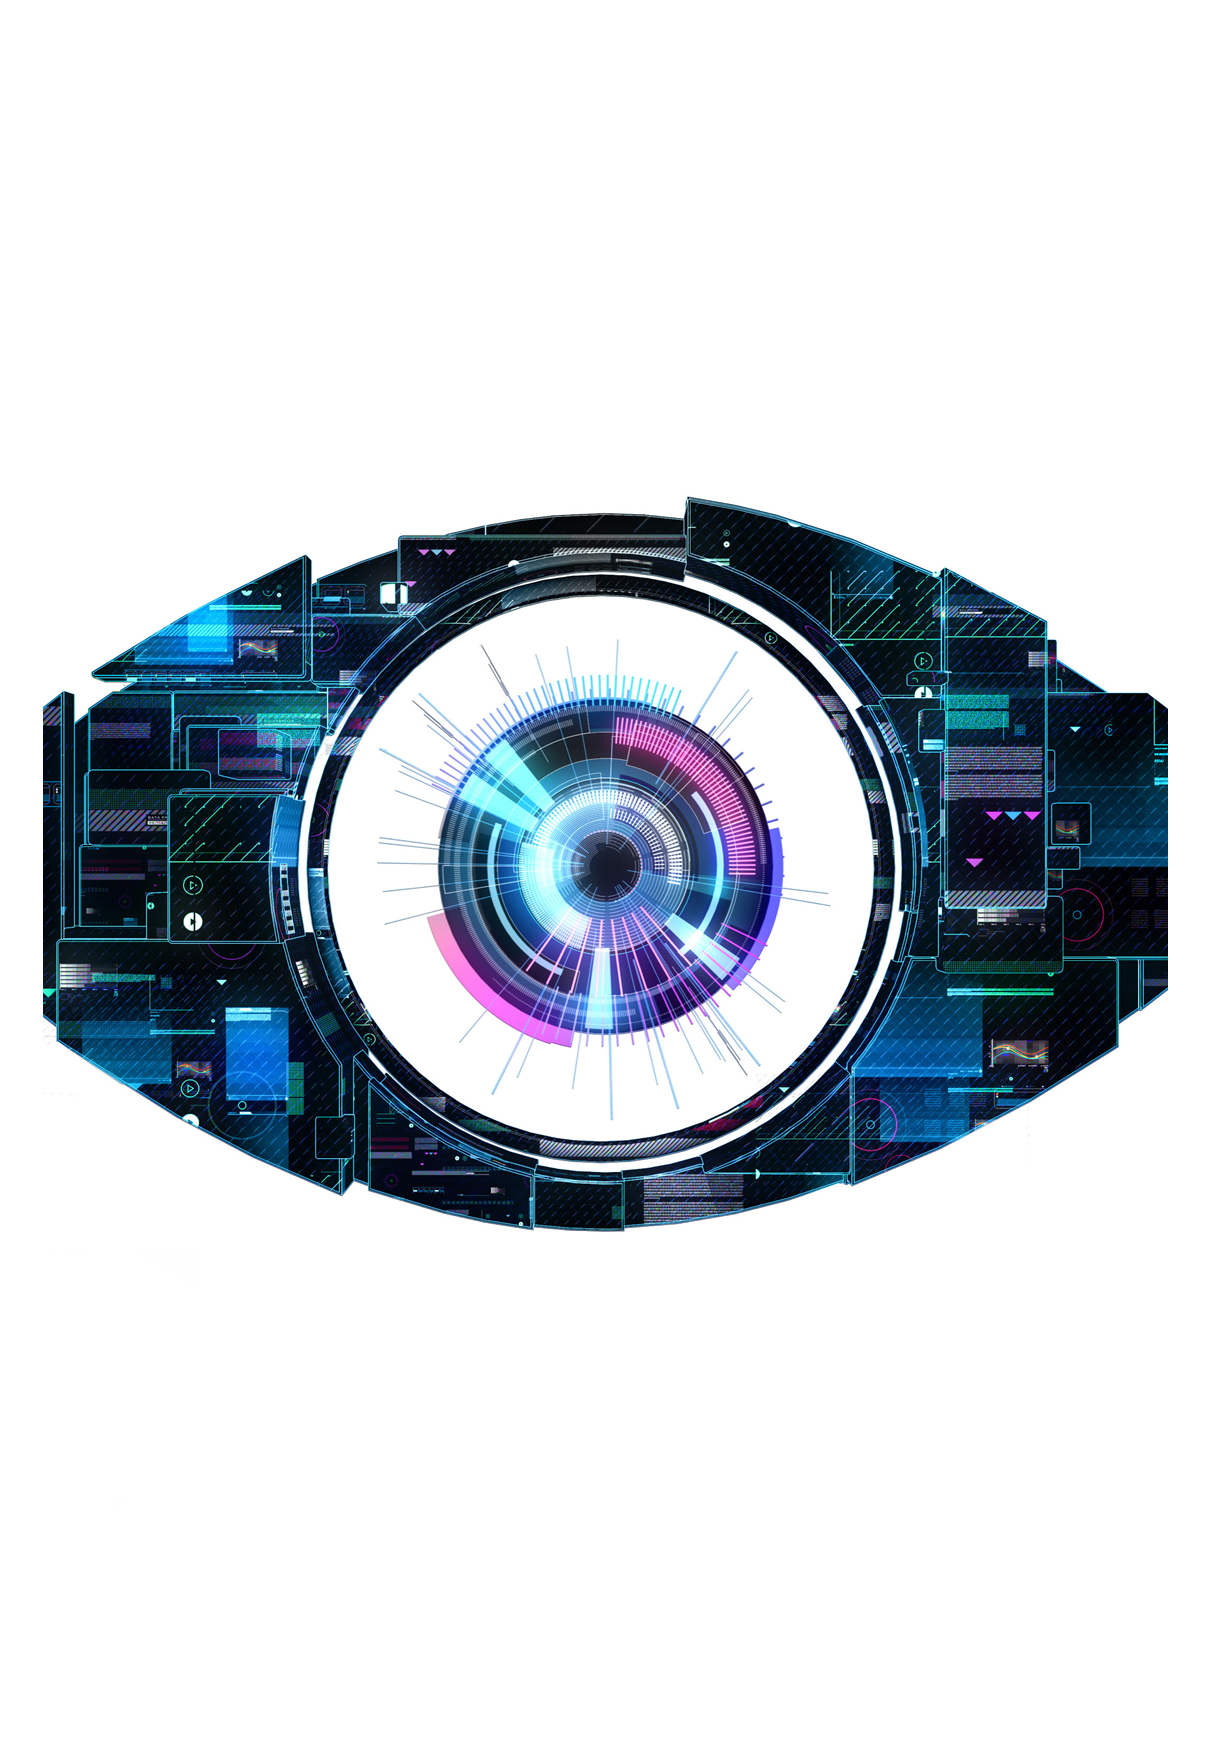
\includegraphics[scale=1]{FrontCover_inside.png}}} % Image background
\centering

\par\normalfont\fontsize{30}{30}\sffamily\selectfont
Google Glass Interaction Techniques for Deaf and Handicapped Users\par % Book title
\vspace*{16cm}

\begin{multicols}{2}
\raggedright
{\huge Workgroup \\ \vspace*{15pt}   \large Ashraf Saleh M. Aly\\ Mohamed Osama\\ Motaz Osama El-Shaer\\ Nourhan Abdelmoneam\\  Sherif El-Sayed Saleh\\ Yahia Attia Nassif\\} % Author name
\columnbreak

{\huge Suepervisors \\ \vspace*{15pt} \raggedright \large Prof.Dr Mohamed A. Ismail \\ Dr. Nagia M. Ghanem\\}
\end{multicols}


\endgroup

%----------------------------------------------------------------------------------------
%	COPYRIGHT PAGE  TODO remove 
%----------------------------------------------------------------------------------------

\newpage
~\vfill
\thispagestyle{empty}

%\noindent Copyright \copyright\ 2013 John Smith\\ % Copyright notice
%\noindent \textsc{Published by Publisher}\\ % Publisher
%\noindent \textsc{book-website.com}\\ % URL
%\noindent Licensed under the Creative Commons Attribution-NonCommercial 3.0 Unported License (the ``License''). You may not use this file except in compliance with the License. You may obtain a copy of the License at \url{http://creativecommons.org/licenses/by-nc/3.0}. Unless required by applicable law or agreed to in writing, software distributed under the License is distributed on an \textsc{``as is'' basis, without warranties or conditions of any kind}, either express or implied. See the License for the specific language governing permissions and limitations under the License.\\ % License information

\noindent \textit{First printing, July 2014} % Printing/edition date

%----------------------------------------------------------------------------------------
%	TABLE OF CONTENTS
%----------------------------------------------------------------------------------------

\chapterimage{cover_8.png} % Table of contents heading image
\pagestyle{empty} % No headers
\tableofcontents % Print the table of contents itself
\cleardoublepage % Forces the first chapter to start on an odd page so it's on the right
\pagestyle{fancy} % Print headers again


%  when testing .. comment all chapters except the chapter you're working on 
\setlength{\parindent}{0pt}


%----------------------------------------------------------------------------------------
%	CHAPTER 0 // Preface
%----------------------------------------------------------------------------------------

\chapterimage{cover1.jpg} % Chapter heading image
\chapter*{Preface}
\section*{Abstract}\index{Abstract}
With the ever-increasing diffusion of wearable computers in our lives, and the increasing time we spend using such devices, developing new techniques that ease interaction with computers has become insistent. One of the most interesting topics in this field is how to allow user to interact with computers without the traditional mode of interaction (mouse, keyboard and even touch-screen). We believe that eye tracking and gesture recognition seem to be very appealing technologies to achieve this goal.\bigskip

Wearable gadgets like Google Glass is a promising example of ubiquitous computers that might be an essential part of our lifestyle in the near future. Glass displays information in a smartphone-like hands-free format, that can communicate with the Internet via natural language voice commands. In this project, two new glass interaction techniques are proposed namely; eye tracking and vision-based gesture recognition.\bigskip

Eye motion tracking serves as powerful tool to know the user's point of gaze and attentional state. Hence this information is used to increase the responsiveness of the computer in respond to users actions. Moreover eye-motions can be translated into commands for Glass. Another feature of eye tracking is that it can be used to provide aid to people with disabilities hindering them from casual interaction with wearable gadgets.\bigskip

Gesture recognition has the potential to be a natural and powerful tool supporting efficient and intuitive interaction between the human and the computer (Glass). Visual interpretation of hand gestures can be interpreted into commands for Glass which definitely will help in achieving the ease and naturalness desired for Human Computer Interaction (HCI). Interpreting sign language is a very promising application of gesture recognition, offering an easy alternative way of interaction that will help many deaf people.
%----------------------------------------------------------------------------------------
%	CHAPTER 1 // Introduction
%----------------------------------------------------------------------------------------
\chapterimage{cover_3.jpg} %TODO change 
\chapter{Introduction}
Our project is based on two techniques, which are eye tracking and gestures recognition. Using these techniques, we can facilitate Human Computer Interaction. This will be very useful for people who have some disabilities. Handicapped who are unable to use their hands to touch the mouse and keyboard can interact with computers using their eye only. With eye tracking, we can detect the gaze point on the screen and determine where the person looks at in order to facilitate the handicapped communication.

The deaf people always use the sign language to interact with the things around them, Depending on the gesture recognition technique, It will be very useful for them to interact with the device using some gestures.

In general our application can make the interaction with the computer or any mobile device becomes easier, Even if the users can have no disabilities. It is very attractive if we use our eye to communicate with the screen or some signs with your hands to move through it, We will have no need for mouse or keyboard or any heavy devices.

\section{Motivation} \index{Motivation}
The Motivation of our system is that we find that we always need to use mouse and keyboard to interact with computer devices such as PC devices and Laptop Devices. With the development in the technology which appears around us every day, the sizes of such devices become smaller and smaller, so we found that there is a motivation to try to find a way by which we could interact with these small devices without need to use other tools to interact with the devices. Therefore we need to cope with the modern technology. \bigskip

On other hand, we need to facilitate human computer interaction to make it easier to interact with the device. It will be attractive if we interact with computer devices with our senses such as eye or hands without using tools to translate what we want to do with the device. There is a pressing need to find a way to facilitate the communication language between the man and the machine. There is a motivation to discover some way to facilitate HCI in general. \bigskip

We use the mouse to move through the screen which gives some commands to the computer device to translate and then process them. Also we use the keyboard to give the commands to the device. How about using our eye to interact with the screen? So the computer device will understand what we want from our eye movement which is extremely comfortable and usable for our needs. So we found that it is a strong motivation to use Eye Tracking Techniques based on Computer Vision. So the communication language between the user and the device is the eye movement which facilitates HCI. Depending on our hands, we can make some signs with our hands according to the action we want to do then, we detect the gesture which is made by hands and translate it to the specific action which facilitates HCI. So our application tries to use our senses to facilitate the way of interaction between the man and the device. \bigskip

Also, there is a serious motivation for our project which is how to make the people who have some disabilities to interact with the computer device without find any difficulties. If this happens, the person with the disability will find it is so easy to use the computer device and interact with it like any person which can develop his abilities and skills. So the most important motivation is to facilitate human computer interaction for people with some disabilities. \bigskip

Handicapped who are unable to use their hands to touch the mouse and keyboard can interact with computers using their eye only. With eye tracking, we can detect the gaze point on the screen and determine where the person looks at in order to facilitate the handicapped communication. \bigskip

Deaf people always use the sign language to interact with  the things around them, Depending on the gesture recognition technique, It will be very useful for them to interact with the device using some gestures. They may not find difficulty to use mouse or keyboard but, when they find that they can interact with the computer device with their familiar language, this will facilitate their interaction and it could be very attractive for them.

\section{Related Work}\index{Related Work}
\subsection{Eye Tracking} \index{Eye Tracking}
Eye tracking is to collect data using either a remote or head-mounted 'eye tracker' connected to a computer. Most generally eye trackers include two common components: a light source and a camera. The light source(usually infra-red) is directed towards the eye. The camera tracks the reflection of the light source along with visible ocular features such as pupil. This data is usually used in estimating gaze of point. \bigskip

There are many different methods for exploring eye tracking data. The most common is to analyze the visual path of one or more participants across an interface such as a computer screen. So, the presence or absence of eye data points in different screen areas can be examined. This type of analysis is used to determine which features are seen, when a particular feature captures attention, how quickly the eye moves, what content is overlooked and virtually any other gaze-related question. \bigskip

Think of all the ways that you will use your eyes today. You might drive a car. You might read a magazine. You might surf the internet or play a video game or complete a training exercise or watch a movie or look at pictures on your mobile device. These are the applications of eye tracking. With very few exceptions, anything with a visual component can be eye tracked. We use our eyes almost constantly, and understanding how we use them has become an extremely important consideration in research and design. \bigskip

Now days, the automotive and medical industries have applied eye tracking technology to make us safer. The fields of advertising, entertainment, packaging and web design have all benefited significantly from studying the visual behaviour of the consumer. Research with special populations has generated exciting breakthroughs in psychology. Every day, as eye tracking is used in creative new ways, the list of applications grows. \bigskip

Today's Eye-tracking algorithms use two main approaches: feature-based and model-based approaches. \bigskip \\
Feature-based approaches detect and localize image features related to position of the eye. There is an important property among all feature-based algorithm which is criteria (e.g. a threshold) needed to decide when a certain feature is present or not. Usually the determination of the criteria or the threshold left to the user. For example on the feature-based algorithm is Starburst because it depends on the corneal reflection. \bigskip \cite{starburst}

On the other hand, model-based approaches don't explicitly detect features but rather find the best fitting model that is consistent with the image. For example Pupil Detection algorithm is model-based approach. However, model-based approaches require searching a complex parameter space that can be fraught with local minima and thus cannot be used without a good initial guess of the model parameters. The gain in accuracy of a model-based approach is obtained at a significant cost in terms of computational speed and flexibility but it is so promise for real-time performance. \bigskip \cite{starburst}

 


\subsection{Starburst}\index{Starburst}
Starburst is a robust algorithm for video based eye tracking. We started with implementing Starburst Algorithm. This algorithm is more accurate than pure feature-based approaches yet is significantly less time consuming than pure model-based approaches. A validation study shows that the technique can reliably estimate eye position with an accuracy of approximately one degree of visual angle even in the presence of significant image noise. \bigskip

The use of eye tracking has significant potential to enhance the quality of everyday human-computer interfaces. Two types of human-computer interfaces utilize eye-movement measures active and passive interfaces. Active interfaces allow users to explicitly control the interface through the use of eye movements. For example, eye-typing applications allow the user to look at keys on a virtual keyboard to type instead of manually pressing keys as with a traditional keyboard. Similarly, systems have been designed that allow users to control the mouse pointer with their eyes in a way that can support, for example, the drawing of pictures. Active interfaces that allow users with movement disabilities to interact with computers may also be helpful for healthy users by speeding icon selection in graphical user interfaces or object selection in virtual reality. Passive interfaces, on the other hand, monitor the user's eye movements and use this information to adapt some aspect of the display. For example, in video transmission and virtual-reality applications, gaze contingent variable-resolution display techniques present a high level of detail at the point of gaze while sacrificing level of detail in the periphery where the absence of detail is not distracting. While eye tracking has been deployed in a number of research systems and to some smaller degree consumer products, eye tracking has not reached its full potential.

\subsection{Robust Realtime Pupil Tracking}\index{Robust Realtime Pupil Tracking}
In this paper, they present a real-time dark-pupil tracking algorithm designed for low-cost head-mounted active-IR hardware. Their algorithm is robust to highly eccentric pupil ellipses and partial obstructions from eyelashes, making it suitable for use with cameras mounted close to the eye. It first computes a fast initial approximation of the pupil position, and performs a novel RANSAC based ellipse fitting to robustly refine this approximation.

\subsection{Pupil}\index{Pupil}
Pupil is an open source platform for pervasive eye tracking and mobile gazed interaction. In this paper, they argue that affordability does not necessarily align with accessibility. They define accessible eye tracking platforms to have the following qualities: open source components, modular hardware and software design, comprehensive documentation, user support, affordable price, and flexibility for future changes. \bigskip

They have developed Pupil, a mobile eye tracking headset and an open source software framework, as an accessible, affordable, and extensible tool for pervasive eye tracking research. They explain the design motivation of the system, provide an in depth technical description of both hardware and software, and provide an analysis of accuracy and performance of the system.

%----------------------------------------------------------------------------------------
%	CHAPTER 2 // Starburst Eye Tracking Algrithm
%----------------------------------------------------------------------------------------
\chapterimage{eyes_women_cropped.jpg}
\chapter{Starburst Eye Tracking Algorithm}
As proposed in the previous chapters that we rely on 2 different approaches to provide a new user experience; Eye-tracking, and gesture recognition. Through this chapter we will go through the details of our eye-tracking module, what algorithms we used, problems we faced, and workarounds to that problems.

\section{Starburst}\index{Starburst}
In the first version of our eye-tracking module we went for implementing the Starburst \cite{starburst}.The Starburst eye-tracking algorithm combines feature-based and model-based approaches to achieve a good trade off between run-time performance and accuracy for dark-pupil infrared illumination. The goal of the algorithm is to extract the location of the pupil center and the corneal reflection so as to relate the vector difference between these measures to coordinates in the scene image. As figure \ref{fig:starburst_overview} shows, the algorithm begins by locating and removing the corneal reflection from the image. Then the pupil edge points are located using an iterative feature-based technique. An ellipse is fitted to a subset of the detected edge points using the Random Sample Consensus (RANSAC) paradigm. The best fitting parameters from this feature-based approach are then used to initialize a local model-based search for the ellipse  parameters that maximize the fit to the image data.


\begin{figure*}[h]
\begin{dBox}
\centering
	\mbox{
		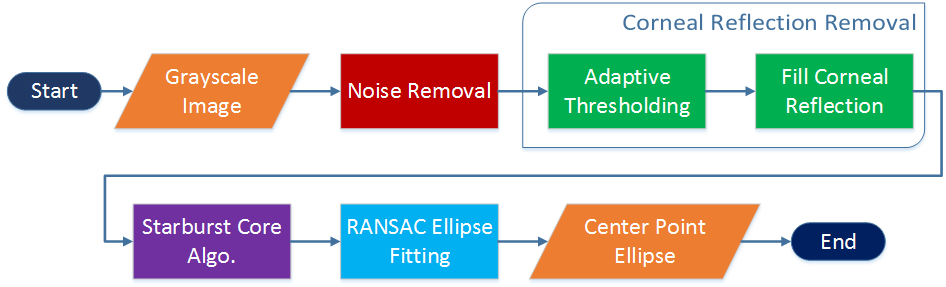
\includegraphics[width=\textwidth]{./Pictures/starburst/Starburst_overview.png}
	}
   \caption{Overview of MIRT Algorithm \label{fig:starburst_overview} }   
\end{dBox}   
\end{figure*}


\section{Noise Reduction}\index{Noise Reduction}
The Starburst algorithms deals with two types of noise that are commonly encountered in any low cost head-mounted eye-tracker. The two types of noise are the shot noise and the line noise. Shot noise is reduced by applying a $5x5$ Gaussian filter with a standard deviation of $2$ pixels. Line noise is reduced by applying a normalization factor is applied line by line shift to shift the mean intensity of the line to the running average derived from previous frames. The following modelling describes the process of line noise reduction as proposed in Startburst \cite{starburst}.

\begin{dBox}
\begin{equation}
	C(i,l) = \beta \bar I  (i,l) + (1 - \beta) C(i-1, l)
\end{equation}
\end{dBox}

Where $C(i,l)$ is the normalization factor, $I(i,l)$ is the average line intensity and $B = 0.2$. Keep in consideration that the noise reduction step is optional and can be deactivated if the used camera is capable of capturing less noisy images.

In our implementation we didn't do any modifications to the noise reduction module. We implemented this module as described in the Starburst algorithm \cite{starburst}. Note that using head-mounted camera in our system doesn't require noise reduction, so this module is deactivated at runtime.


\section{Corneal Reflection}\index{Corneal Reflection}
\subsection{Detection and Localization}\index{Detection and Localization}

The corneal reflection corresponds to one of the brightest regions in the eye image. Thus the corneal reflection can be obtained through thresholding. However, a constant threshold across observers and even within observers is not optimal. Therefore we use an adaptive thresholding technique in each frame to localize the corneal reflection. \bigskip

One of the heuristics adopted by the Starburst algorithm is that cornea extends approximately to the limbus, so the search space for the cornea can be limited with a square region of interest by half width of $h = 150$ which makes sense. Other heuristic which we believe is the core of the corneal reflection detection is that the corneal reflection is the largest and the brightest candidate region in the region of interest, as other specular reflections tend to be quite small and located off the cornea as well as near the corner of the image where the eye lids meet. \bigskip

At first the input (gray scale) frame is converted to binary form, only values above the maximum threshold are taken as corneal reflection candidates. Then the ratio between the area of the largest candidate to the average area of other regions is calculated as the threshold is lowered. A notable observation is that the intensity of the corneal reflection monotonically decreases towards the edges.\bigskip

At the beginning the ratio between  largest candidate area and average area of other candidates will increase since the corneal reflection will grow in size faster than other areas. As the threshold is decreased the ratio will begin to drop because the false candidates are becoming of significant size compared to the corneal reflection. The optimal threshold is the threshold that generates the hight ratio. The largest candidate using the optimal threshold is considered the corneal reflection with the geometric center $(c_{x}, c_{y})$. \bigskip

In the Starburst algorithm the corneal reflection intensity profile is assumed to follow a bivariate Gaussian distribution. Full extent of the corneal reflection is obtained by relating the the radius $r$ where the average decline in intensity is maximal to the radius with maximal decline for a Gaussian (i.e. a radius of one standard deviation). To capture 99\% of the corneal reflection profile use $2.5r$. Where $r$ is computed through a gradient decent search that minimizes:


\begin{dBox}
	\begin{equation}
		\frac{ \int I ( r + \delta, x_{c}, y_{c}, \theta ) d\theta }{ \int I ( r - \delta, x_{c}, y_{c}, \theta ) d\theta}
	\end{equation}
\end{dBox}

where $\delta = 1$ and $I(r, x, y, \theta)$ is the pixel intensity at angle $\theta$ on the contour of a circle defined by the parameters $r$, $x$, and $y$. The search is initialized with $r = \sqrt{area/\pi}$, where area is the number of pixels in the thresholded region. The search converges rapidly.\bigskip

In our implementation we used a simplified version for corneal reflection detection procedure described by the Starburst algorithm. First step we convert the input gray scale image to binary form. Then we perform adaptive thresholding until we find the optimal threshold (which generates the highest ratio) as described in the original algorithm. Next we estimate the the center of corneal reflection region. Till now no differences from the original algorithm. The main difference is that we assume that the corneal reflection is circular and hence we find the radius from the area of circle relation $r = \sqrt{ area_{max} / \pi }$.

\subsection{Removal}\index{Removal}
Original Starburst algorithm uses radial interpolation to remove the corneal reflection. First, the central pixel of the identified corneal reflection region is set to the average of the intensities along the contour of the region. Then for each pixel between the center and the contour, the pixel intensity is determined via linear interpolation. \bigskip

Our implementation of the corneal reflection removal is different to the original algorithm, we assume that the corneal reflection is circular and hence we fill a circular region in the image with an estimation of the pupil intensity. The pupil intensity is estimated by averaging the intensity along the ring that encapsulates the corneal reflection and is $d$ pixels larger than corneal reflection radius, where $d$ is set to 10 pixels.



\section{Starburst Algorithm}\index{Starburst Algorithm}

Unlike most of feature based eye tracking approaches that apply edge detection to the entire image, Starburst algorithm detects edges along a limited number of rays that extend from a central best guess of the pupil center. These rays can be seen in Figure \ref{pupil_rays}. This method takes advantage of the high-contrast elliptical profile of the pupil contour present in images taken using the dark-pupil technique. Algorithm pseudo code is shown in algorithm \ref{starburst_psuedo}. \bigskip


\begin{algorithm}
\begin{dBox}
	\caption{Starburst Original Algorithm} \label{starburst_psuedo}
	\begin{algorithmic}[1]
		\Require{Eye image - corneal reflection removed, Best guess of pupil center}
		\Ensure {Set of feature points}
		\Procedure{Starburst}{}
			\Repeat  
				\vspace{1em}	
				\State \emph{Stage 1:}
					\State Follow rays extending from the starting point
					\State Calculate intensity derivative at each point
					\If {$derivative > threshold$} 
						\State Place feature point
						\State Halt marching along ray
					\EndIf		
				\vspace{1em}	
				\State \emph{Stage 2:}
					\ForAll {feature points detected in Stage 1}
						\State March along rays returning towards the start point
						\State Calculate intensity derivative at each point
						\If {$derivative > threshold$} 
							\State Place feature point
							\State Halt marching along ray
						\EndIf		
					\EndFor
					\vspace{.3em}			
					\State Starting point = geometric center of feature points
			\vspace{1em}							
			\Until{starting point converges}
		\EndProcedure	
	\end{algorithmic}
\end{dBox}	
\end{algorithm}

For each frame a location is chosen that represent the best guess of the pupil center in this frame. The best guess at the first frame is chosen to be the center of the image, best guess at frame $i$ are set to be the center of the pupil detected in the previous frame (frame $i-1$).  Next, the derivatives $\vartriangle$ along the $N = 18$ rays, extending radially away from this starting point, are independently evaluated pixel by pixel until a threshold $\phi = 20$ is exceeded. Since Starburst uses a dark-pupil technique, only positive derivatives (increasing intensity as the ray extends) are considered. When the value of the derivative along the line exceeds the threshold a features point (pupil edge candidate point) is marked, and the processing along this line is halted. If the processing along a line reached borders of the image no feature point is marked. Example of the candidate feature points and corresponding rays are shown at figure \ref{fig:starburst_example}. \bigskip


\begin{figure*}[]
\begin{dBox}
\centering
  \mbox{
      \subfigure[Stage 1 rays]{
            \label{fig:stage_1}
            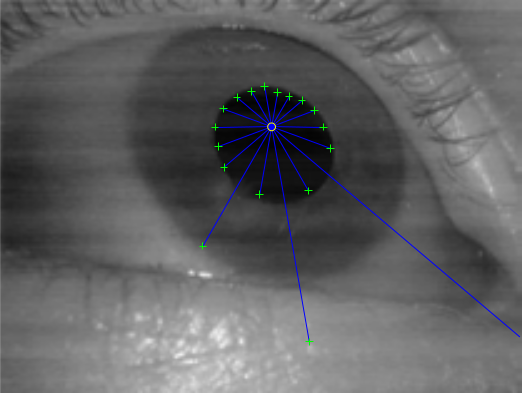
\includegraphics[width=.31\textwidth]{./Pictures/starburst/3a.png}
        }
        \subfigure[Stage 2 inlier point]{
           \label{fig:stage_2_inlier}
           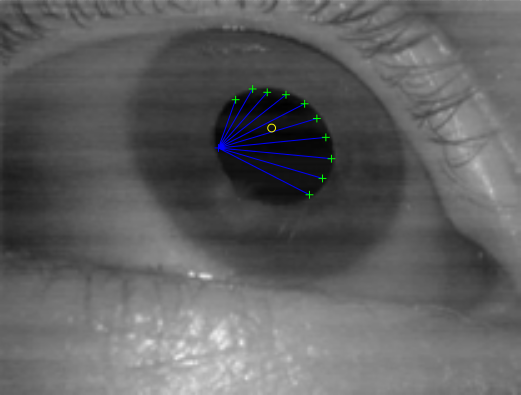
\includegraphics[width=.31\textwidth]{./Pictures/starburst/3b.png}
        }
        \subfigure[Stage 2 outlier point]{
            \label{fig:stage_2_outlier}
            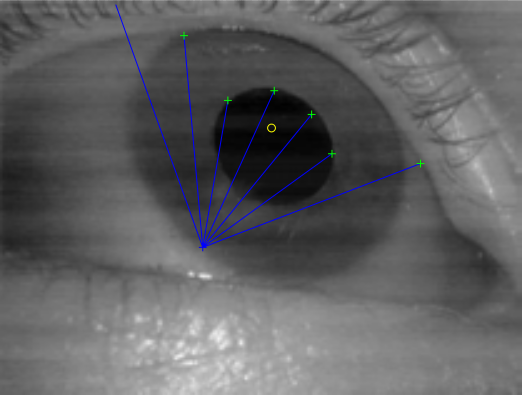
\includegraphics[width=.31\textwidth]{./Pictures/starburst/3c.png}
       }
   }
   \caption{Visualization of Starburst stage 1 and stage 2 feature point detection procedure \label{fig:starburst_example} }   
\end{dBox}   
\end{figure*}

For every feature point obtained the above described algorithm is repeated with a minor modification. Search rays are limited to $\gamma = \pm 50$ degrees from the original ray that originally produced the feature point. This procedure tends to increase the ratio of the number of feature points on the pupil contour over the number of feature points not on the pupil contour. If the pivot feature point lies on the pupil contour then the rays around the original ray will result in feature points that also lie on the opposite half of the pupil contour. On the other hand if the original feature point is not on the pupil contour, then limiting the search space will cut down the number of feature point that doesn't lie on the pupil contour. One important note to take into consideration is that the number of rays in this step is only 10 (5 on each side of the original ray). Figure \ref{fig:starburst_stage2_example} shows the two cases described above. \bigskip



\begin{figure*}[h]
\begin{dBox}
\centering
  \mbox{
        \subfigure[Stage 2 inlier point]{
           \label{fig:stage_2_inlier_p}
           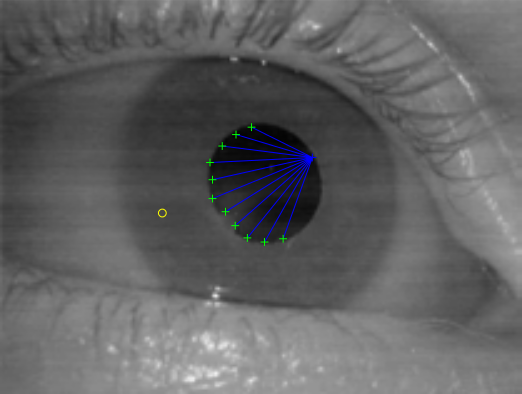
\includegraphics[width=.31\textwidth]{./Pictures/starburst/4b.png}
        }
        \subfigure[Stage 2 outlier point]{
            \label{fig:stage_2_outlier_p}
            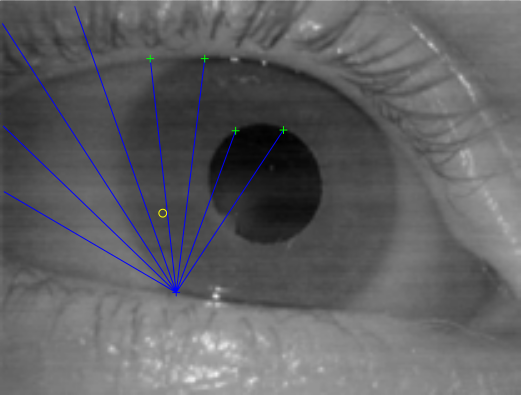
\includegraphics[width=.31\textwidth]{./Pictures/starburst/4c.png}
       }
   }
   \caption{Visualization of Starburst stage 2 feature point detection procedure \label{fig:starburst_stage2_example} }   
\end{dBox}   
\end{figure*}

Using the two stage feature detection process improves the robustness of the method to poor initial guesses for the starting point. However, the feature points tend to bias to the side of the pupil contour nearest the initialization point. Although another iteration of the ray process would minimize this bias, the computational burden grows exponentially with each iteration and thus would be an inefficient strategy. \bigskip

Fitting an ellipse to the set of biased feature points will induce significant error into fit. A good strategy to eliminate the bias is to iterate the recently described procedure, with each time computing the average of the detected feature points to be the new estimated center of the pupil for the next iteration. The iterating process is halted when the estimated pupil center between two successive iteration is less than $d = 10$ pixels. Starburst paper mention that if guess is a good estimate of the pupil center, only a single iteration is required. When the initial estimate is not good, typically only a few iterations ($< 5$) are required for convergence. If convergence is not reached within $i = 10 $iterations, as occurs sometimes during a blink when no pupil is visible, the algorithm halts and begins processing the next frame. \bigskip

In out implementation of this module we sticked to the exact Startburst algorithm described in the paper.



\section{Ellipse Fitting}{Ellipse Fitting}
Given a set of feature points, the function of this module is to find best fitting ellipse.  Most of algorithms use least-squares ellipse fitting including all feature points (e.g. see \cite{least_squares}). Using all points to estimate an ellipse results in significant error that strongly affect the accuracy. Notice that a few feature points not on the pupil contour dramatically reduces the quality of the fit to an unacceptable level.  \bigskip

To address this issue Starburst uses Random Sample Consensus (RANSAC) paradigm for model fitting \cite{ransac}. Starburst paper claims that Starburst is the first algorithm that uses RANSAC in the context of eye-tracking. RANSAC is an effective technique for model fitting in the presence of a large but unknown percentage of outliers in a measurement sample. A basic assumption is that the data  consists of "inliers", i.e., data whose distribution can be explained by some set of model parameters, though may be subject to noise, and "outliers" which are data that do not fit the model. In our application inliers are feature points that lie on the pupil contour, while outliers are feature points that belong to other contours other than the pupil contour. Least-squares approaches assumes that all sample points fit the model and hence, uses all the sample points to estimate the model. On the other hand RANSAC is an iterative method to estimate parameters of a mathematical model from a set of observed data which contains outliers. General outline of RANSAC technique is shown at algorithm \ref{ransac_outline}. \bigskip

\begin{algorithm}
\begin{dBox}
	\caption{General RANSAC Procedure} \label{ransac_outline}
	\begin{algorithmic}[1]
		\Procedure{RANSAC}{}
		 \While{$i < N$}
			\State Draw $s$ points uniformly at random
			\State Fit model to these $s$ points
			\State Find inliers to this model among the remaining points (points whose error $ < t$)
			\State If there are $d$ or more inliers, accept the model and refit using all inliers	
		\EndWhile	
		\EndProcedure	
	\end{algorithmic}
\end{dBox}	
\end{algorithm}


The output of the two stage feature detection process may result in very few outliers in some cases, while in other cases outlier prevail. Using the RANSAC technique increase the ability of the system to do robust estimation of the model (ellipse) parameters. The following procedure is repeated $R$ times. First, five samples are randomly drawn from the set of feature set obtained by the previous module.  Singular Value Decomposition (SVD) on the conic constraint matrix generated with normalized feature-point coordinates \cite{multipleViewGeom} is used to find the parameters of the ellipse that perfectly fit these five points. Then, the number of candidate feature points in the data set that agree with this model (i.e. the inliers) are counted. Inliers are those sample points for which the algebraic distance to the ellipse is less than some threshold $t$. \bigskip

Our implementation of this stage differs a bit from the implementation of the original Starburst. We draw 5 samples from the detected feature set, then we compute the best fit ellipse using Fitzgibbon's algorithm \cite{fitzgibbon96} which is implemented in OpenCV. Finally we evaluate the error between the estimated model and all feature points and count inliers/outliers. Algorithm \ref{our_ransac_outline} summarizes how we use RANSAC in our system. \bigskip

\begin{algorithm}
\begin{dBox}
	\caption{Our RANSAC Procedure} \label{our_ransac_outline}
	\begin{algorithmic}[1]
		\Procedure{RANSAC}{}
		 \While{$i < N$}
			\State Draw $s$ points uniformly at random
			\State Fit ellipse model to these $s$ points
			\State Find inliers to this ellipse (points whose algebraic error $ < t$)
			\State If there are $d$ or more inliers, accept the ellipse and refit using all inliers	
		\EndWhile	
		\EndProcedure	
	\end{algorithmic}
\end{dBox}	
\end{algorithm}


As a matter of fact we tried different approaches in our implementation, at first we tried to implement the same approach mentioned in the Starburst paper. However finding the SVD of the parameter matrix using OpenCV SVD didn't produce consistent results because the calculated eigen vectors/values were not correct. Some books like \cite{practicalOpenCV} addressed this issue and suggested using Eigen mathematics library \cite{eigenweb} to find the eigen values/vector. In our application we couldn't benefit from this solution since, Eigen library is only available in C++ while the user end if our application is in Java (Android user end).


\subsection{Estimation of Number of Iterations $R$}\index{Number of Iterations}
Starbusrt algorithm assumes that the average error variance of the feature detector is approximately one pixel and that this error is distributed as a Gaussian with zero mean. Thus to obtain a 95\% probability that a sample is correctly classified as an inlier, the threshold should be derived from a $\chi^{2}$ distribution with one degree of freedom \cite{multipleViewGeom}. This results in a threshold distance of $t = 1.98$ pixels. \bigskip

The parameter R (the number of iterations), however, can be determined from a theoretical result. Let p be the probability that the RANSAC algorithm in some iteration selects only inliers from the input data set when it chooses the $s$ points from which the model parameters are estimated. When this happens, the resulting model is likely to be useful so $p$ gives the probability that the algorithm produces a useful result. Let $w$ be the probability of choosing an inlier each time a single point is selected, that is, 
\begin{dBox}
	$$ w = \frac{number \: of \: inliers \: in \: data}{number \: of \: points \: in \: data} $$
\end{dBox}
it can be proven that 
\begin{dBox}
\begin{equation}
		R = \frac{log(1-p)}{log(1-w^{5})}
\end{equation}
\end{dBox}

\section{Homographic Mapping and Calibration}\index{Homographic Mapping and Calibration}
In order to calculate the point of gaze of the user in the scene image, a mapping between locations in the scene image and an eye-position measure must be determined. The typical way to determine the mapping is via a calibration process. During calibration, the user is required to look at a number of scene points for which the positions in the scene image are known. At each position the eye-position $\vec{e} = (x_{e} ,\: y_{e},\: 1)$ and the scene position $\vec{s} = (x_{s},\: y_{s},\: 1)$ is measured. The mapping is generated using the $3x3$ Homography matrix which has 8 degrees of freedoms. Each point (map from scene to eye) produces 2 independent equations. Hence four mapping points are needed to compute the entries of the homography matrix up to scale \cite{heuristic}. \bigskip

In our implementation we use the OpenCV \textit{findHomography} procedure to find the homography matrix. Given a set of points in image coordinates and corresponding set of points in the eye coordinates, \textit{findHomography} finds a perspective transformation between two coordinate systems. \bigskip

Once this mapping is determined the user’s point of gaze in the scene for any frame can be established
as $\vec{s} = H \vec{e}$.

%----------------------------------------------------------------------------------------
%	CHAPTER 3 // Pupil Eye Tracking Algrithm
%----------------------------------------------------------------------------------------
\chapterimage{Pupil_Chapter_photo4.jpg}
\chapter{Pupil Eye Tracking Algorithm}
As proposed in the previous chapters that we rely on Starburst \cite{starburst} Algorithm to get the center of the pupil. But we found that Starburst is not robust and accurate, so we will use Pupil Algorithm to enhance eye-tracking module. Through this chapter we will go through the details of our eye-tracking module by using Pupil Algorithm.

\section{Pupil}\index{Pupil}
In the second version of our eye-tracking module we went for implementing the Pupil Algorithm \cite{pupil}. Pupil eye-tracking algorithm is an accessible, affordable and extensible tool for pervasive eye tracking research. This chapter we will explain the design motivation of the algorithm, provide an in depth technical description of algorithm. We will use a wearable mobile eye tracking headset with one 
scene camera and one infra-red (IR) spectrum eye camera for dark pupil detection. Both cameras connect to a laptop, desktop, or mobile computer platform via high speed USB 2.0. The camera video streams are read for real-time pupil detection, gaze mapping and recording.  


\section{System Design Objectives}\index{Pupil}
	Pupil leverages the rapid development cycle and scaling effects of consumer electronics, USB cameras and consumer computing hardware, instead of using custom cameras and computing solutions. \bigskip

Pupil algorithm is open source and strives to build and support a community of eye tracking researchers and developers.

\section{Cameras} \index{Cameras}
The scene camera mount and eye camera mount interface geometries are open source. By releasing the mount geometry we automatically document the interface, allowing users to develop their own mounts for cameras of their choice. \bigskip

Pupil uses USB interface digital cameras that comply with the UVC (USB Video Class) standard. The Pupil headset can be used with other software that supports the UVC interface. Pupil can be easily extended to use two eye cameras for binocular set-ups and more scene cameras as desired. 

\subsection{Eye Camera} \index{Eye Camera}
We use a small and lightweight eye camera to reduce the amount of visual obstruction for the user and keep the headset lightweight. The eye camera can capture at a maximum resolution of 800x600 pixels at 30 Hz. Using an IR mirror ("hot mirror") was considered as  strategy to further reduce visual obstruction. 

\bigskip
 Pupil uses the "dark pupil" detection method. This Requires the eye camera to capture video within a specific range of the IR spectrum. 
 
 \subsection{Scene Camera} \index{Eye Camera}
  The scene camera is mounted above the user’s eye aligning the scene camera optics with the user’s eye along a sagittal plane. The scene camera faces outwards to capture a video stream of a portion of the users FOV at 30Hz. The scene camera lens has a 90 degree diagonal FOV. The scene camera is not only high resolution (max resolution 1920x1080 pixels), but also uses a high quality image sensor. This is very
advantageous for further computer vision and related tasks
performed in software.


\section{Computing Device} \index{Computing Device}
The Pupil eye tracking algorithm works in conjunction with standard multi-purpose computers: laptop, desktop, or tablet. Designing for user supplied recording and processing hardware introduces a source for compatibility issues and requires more set-up effort for both users and developers. However, enabling the user to pair the headset with their own computing platform makes Pupil a multi-purpose eye tracking and analysis tool. Pupil is deployable for lightweight mobile use as well as more specialized applications like: streaming over networks, geotagging, multi-user synchronization; and computationally intensive applications like real time 3D reconstruction and localization.

\section{Pupil Detection Algorithm} \index{Pupil Detection Algorithm}
The pupil detection algorithm locates the dark pupil in the IR illuminated eye camera image. The algorithm does not depend on the corneal reflection, and works with users who wear contact lenses and eyeglasses. \bigskip

The pupil detection algorithm is under constant improvement based on feedback collected through user submitted eye camera videos. Here we provide a description of default pupil detection algorithm.
\bigskip

\subsection{overview} \index{Pupil Detection Algorithm}
The eye camera image is converted to gray-scale. The initial region estimation of the pupil is found via the strongest response for a center-surround feature as proposed by Swirski et al. \cite{swirski} within the image. \newline  

Detect edges using Canny \cite{canny} to find contours in eye image. Filter edges based on neighbouring pixel intensity. Look for darker areas (blue region). Dark is specified using a user set offset of the lowest spike in the histogram of pixel intensities in the eye image. \\*

Filter remaining edges to exclude those stemming from spectral reflections. Remaining edges are extracted into into contours using connected components \cite{suzuki}. Contours are filtered and split into sub-contours based on criteria of curvature continuity. \\*

Candidate pupil ellipses are formed using ellipse fitting \cite{fitzgibbon96} onto a subset of the contours looking for good fits in a least square sense, major radii within a user defined range, and a few additional criteria. \\* 

The results are evaluated based on the ellipse fit of the supporting edges and the ratio of supporting edge length and ellipse circumference (using Ramanujans second approximation \cite{hardy1962collected} ). We call this ratio "confidence". If the best results confidence is above a threshold the algorithm reports this candidate ellipse as the ellipse defining the contour of the pupil. Otherwise the algorithm reports that no pupil was found.\\*

\begin{figure*}[]
\begin{dBox}
\centering
  \mbox{
	    \subfigure[Algorithm Overview]{
            \label{fig:overview}
            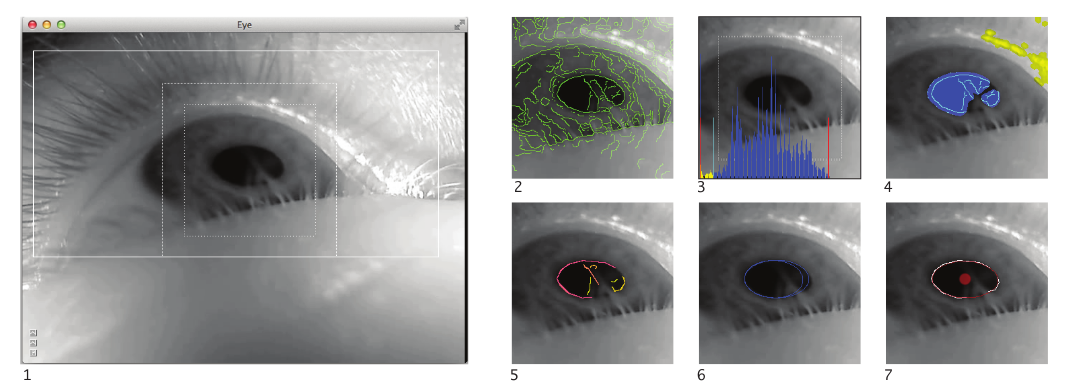
\includegraphics[width=1.0\textwidth]{./Pictures/Visulaization_of_Pupil_algo.png}
        }
   }
   \caption{Vizualization of pupil detection algorithm. 1) Eye image converted to gray scale, user region of interest (white stroke rectangle), and initial estimation of pupil region (white square and dashed line square.) 2) Canny edge detection (green lines). 3) Define "dark" region as offset from lowest spike in histogram within eye image. 4) Filter edges to exclude spectral reflections(yellow) and not inside "dark" areas (blue). 5) Remaining edges extracted into contours using connected components and split into sub-contours based on curvature criteria (multi colored lines). 6) Candidate pupil ellipses (blue) are formed using ellipse fitting. 7) Final Ellipse fit found through an augmented combinatorial search( finally ellipse with center in red)-supporting edge pixels drawn in white.
 \label{fig:Pupil_Performance} }   
\end{dBox}   
\end{figure*}


\begin{figure*}[]
\begin{dBox}
\centering
  \mbox{
	      \subfigure[Comparison]{
            \label{fig:Comparison}
            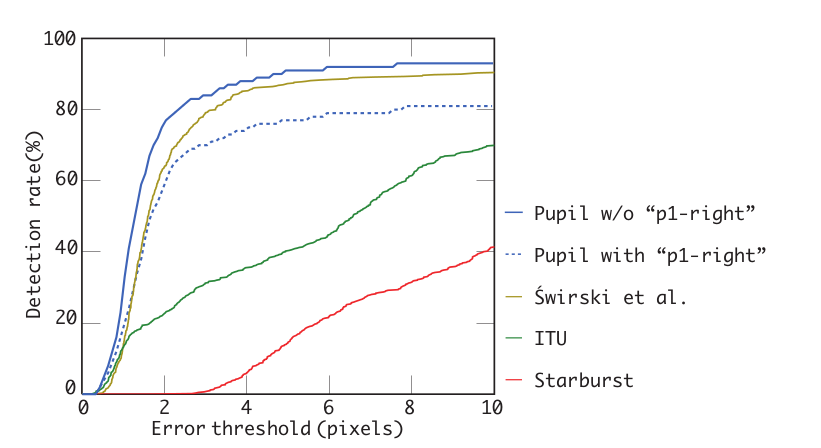
\includegraphics[width=.80\textwidth]{./Pictures/comparison.png}
        }
   }
   \caption{Comparison of pupil detection rate for Pupil’s algorithm, the stock algorithm proposed by Swirski et al., the ITU gaze tracker and Starburst.
 \label{fig:Pupil_Performance} }   
\end{dBox}   
\end{figure*}

Figure \ref{fig:Pupil_Performance} shows a performance comparison between Pupil’s pupil detection algorithm, the stock algorithm proposed by Swirski et al., the ITU gaze tracker and Starburst on the benchmark dataset by Swirski et al. \cite{swirski}. As error measure we used the Hausdorff distance between the detected and hand-labeled pupil ellipses \cite{swirski}. We additionally conducted a test excluding the dataset p1-right, that contains eye images recorded at the most extreme angles.
As can be seen from the Figure, Pupil without p1-right compares favourably to all other approaches. With an error threshold of 2 pixels Pupil achieves a detection rate of 80\%; at 5 pixels error detection rate increases to 90\%

\begin{figure*}[]
\begin{dBox}
\centering
  \mbox{
	      \subfigure[Initial Estimation of Pupil Region]{
            \label{fig:Pupil Region}
            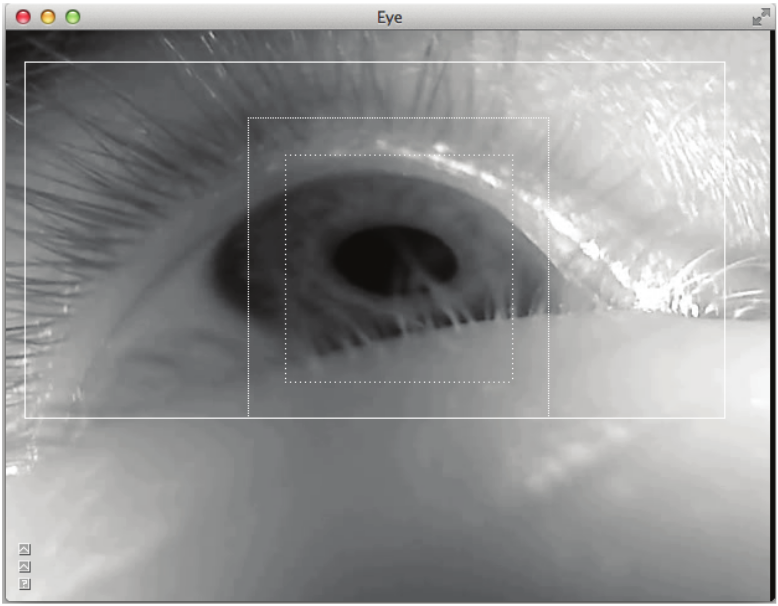
\includegraphics[width=.80\textwidth]{./Pictures/initial_estimation_of_pupil.png}
        }
   }
   \caption{ User region of interest (white stroke rectangle), and initial estimation of pupil region (white square and dashed line square.)
 \label{fig:Pupil Region} }   
\end{dBox}   
\end{figure*}


\begin{figure*}[]
\begin{dBox}
\centering
  \mbox{
	      \subfigure[Estimation of Pupil Region]{
            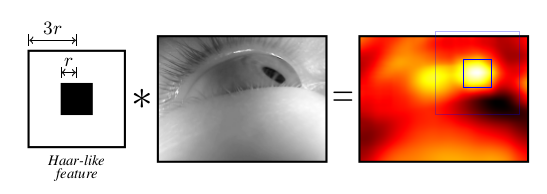
\includegraphics[width=.80\textwidth]{./Pictures/estimation_pupil_region.png}
        }
   }
   \caption{ To find the approximate pupil region, the eye image is convolved with a Haar-like centre surround feature of radius r. The pupil region is centred on the location of the maximal response over all pixels and radii
 \label{fig:EstimationPupilFig} }   
\end{dBox}   
\end{figure*}


\begin{figure*}[]
\begin{dBox}
\centering
  \mbox{
	      \subfigure[]{
            \label{fig:IntegralImage}
            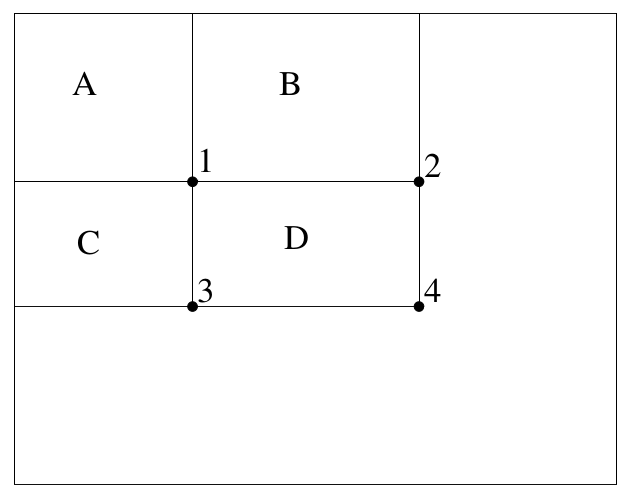
\includegraphics[width=.40\textwidth]{./Pictures/integral_image.png}
        }
   }
   \caption{ To find the approximate pupil region, the eye image is convolved with a Haar-like centre surround feature of radius r. The pupil region is centred on the location of the maximal response over all pixels and radii
 \label{fig:IntegralFig} }   
\end{dBox}   
\end{figure*}


\subsection{Integral Image} \index{ Pupil Detection Algorithm }
Rectangle features can be computed very rapidly using an intermediate representation for the image which we call the integral image. The integral image at location $x, y$ contains the sum of the pixels above and to the left of $x, y$, inclusive: \\
\begin{center}
$ii(x,y)=\sum\limits_{x'<=x,y'<= y}i(x', y')$,
\end{center}
where $ii(x,y)$ is the integral image and $i(x,y)$ is the original image. Using the following pair of recurrences:
\begin{center}
	\begin{equation}
	$s(x,y) = s(x,y-1)+ i(x,y)$
	\end{equation}

	\begin{equation}
	$ii(x,y) = ii(x-1,y)+ s(x,y)$
	\end{equation}

\end{center}
(where $ s(x,y) $is the cumulative row sum, $s(x, -1) = 0$, and $ii(-1, y) == 0$) the integral image can be computed in one pass over the original image. \\
Using the integral image any rectangular sum can be computed in four array references figure \ref{fig:IntegralFig}. Clearly the difference between two rectangular sums can be computed in eight references. Since the two-rectangle features defined above involve adjacent rectangular sums they can be computed in six array references, eight in the case of the three-rectangle features, and nine for four-rectangle features.\cite{ViolaAndJones2001}

\begin{figure*}[]
\begin{dBox}
\centering
  \mbox{
	      \subfigure[Original Eye Image]{
	            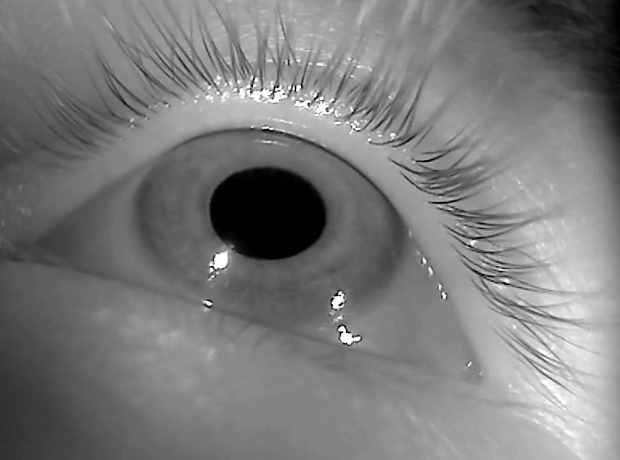
\includegraphics[width=.45\textwidth]{./Pictures/0-eye.png}
        }
	      \subfigure[Region of interest(ROI) after Running Initial Estimation Of Pupil Module]{
	      		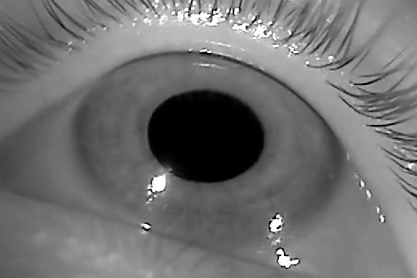
\includegraphics[width=.50\textwidth]{./Pictures/ROI.png}
        }
   }
   
   \caption{Input \& Output of Initial Estimation of Pupil Module. \label{fig:Initial_Estimation_Of_Pupil} }   
\end{dBox}   
\end{figure*}

\subsection{Initial Estimation Of Pupil} \index{Pupil Detection Algorithm}
Our initial region estimation assumes that the pupil region, either the dark pupil itself or the combination of pupil and iris, can roughly be described as a “ dark blob surrounded by a light background ”, and is the strongest such feature in the image. To find the pupil, we use a Haar-like feature detector, similar to the features used in cascade classifiers \cite{ViolaAndJones2001}. \bigskip

The core idea of the feature detector can be explained in terms of convolution. To find possible pupil regions, we convolve the image with a Haar-like centre-surround feature of a given radius figure \ref{fig:EstimationPupilFig} . We repeat this for a set of possible radii, between a user specified minimum and maximum, and find the strongest response over the 3D space of (x, y) and radii. The (x, y) location of this strongest response is assumed to be the centre of the pupil region, with the size of the region determined by the corresponding radius. \bigskip

Although such a convolution is a slow operation if performed naively, we optimise this by first calculating the integral image \cite{ViolaAndJones2001}. Using this integral image, we can find the response of a pixel to a Haar-like feature in constant time, only needing to sample 8 pixel values, one for each corner of the two squares, thereby making this step linear in the number of pixels and possible radii. \\
Input and Output of this module is shown in Figure \ref{fig:Initial_Estimation_Of_Pupil}

\begin{figure*}[]
\begin{dBox}
\centering
  \mbox{
	      \subfigure[Eye Image after Computing Histogram]{
	            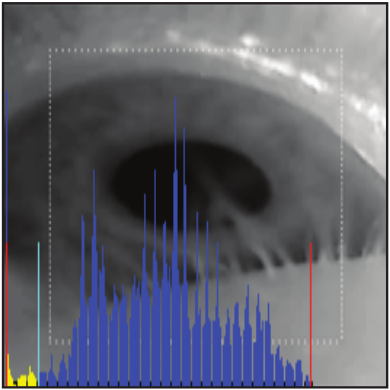
\includegraphics[width=.40\textwidth]{./Pictures/histogramOnDarkRegion.png}
        }
   }
   \caption{After Computing Histogram to get Spikes. 
   \label{fig:HistogramOnEyeImage} }   
\end{dBox}   
\end{figure*}

\begin{figure*}[]
\begin{dBox}
\centering
  \mbox{
	    \subfigure[Eye image after applying Closing operation on Eye image.]{
	          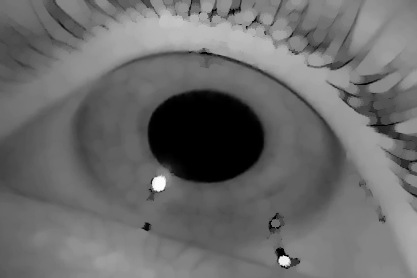
\includegraphics[width=.60\textwidth]{./Pictures/dark_region_img.png}
        }
        	\subfigure[Dark region is indicated by the Blue Region]{
        		  \label{fig:SpectralReflection} 
	          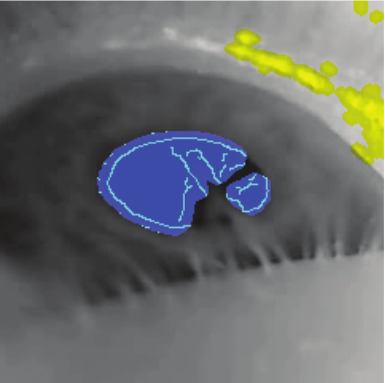
\includegraphics[width=.40\textwidth]{./Pictures/DarkRegion.png}
        }

   }
   \caption{After Applying Morphological operations(Closing operations). 
   \label{fig:DarkImageInBlue} }   
\end{dBox}   
\end{figure*}


\begin{figure*}[]
\begin{dBox}
\centering
  \mbox{
	    \subfigure[Eye image after applying Closing operation on Eye image.]{
	          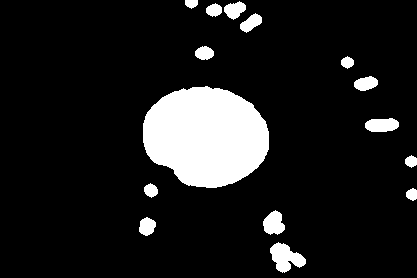
\includegraphics[width=.30\textwidth]{./Pictures/dark_region_binary_img.png}
        }
   }
   \caption{Final Result of Getting Dark Region Module. 
   \label{fig:DarkImageInBinary} }   
\end{dBox}   
\end{figure*}


\subsection{Getting Dark Region(Pupil Region)} \index{Pupil Detection Algorithm}
Here we want to extract the region which include the pupil by getting the most dark region in eye image. And then we filter the eye image by applying some Morphological operations like Dilation and Erosion to remove the noise to get a pure dark region. \bigskip

At first we should get the histogram of the gray image of Region Of Interest (ROI) which we get from Initial Estimation Of Pupil Module. Then we should deduce spikes from histograms. After getting the lowest and highest spikes in histogram we can get the binary image of ROI by using lowest spike +  user offset(usually we set offset by 11) as threshold as shown in figure \ref{fig:HistogramOnEyeImage}. \bigskip

Then, we should do some Morphological operation on binary image. to filter the image from any noise and make contours more clearer, so we apply Erosion at first and then Dilation(Closing Operation) as shown in Figure \ref{fig:DarkImageInBlue}. \bigskip

Finally we get the ROI as a binary image include only the Dark Region which represents Pupil as shown in Figure \ref{fig:DarkImageInBinary}.


\begin{figure*}[]
\begin{dBox}
\centering
  \mbox{
	    \subfigure[Edges of eye image after Excluding Spectral Reflections]{
	          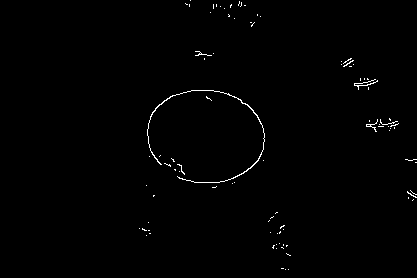
\includegraphics[width=.50\textwidth]{./Pictures/edges_after_Removing_Spectral_Refl.png}
        }
   }
   \caption{Final Result of Excluding Spectral Reflection module.
   \label{fig:Edges} }   
\end{dBox}   
\end{figure*}

\subsection{Excluding Spectral Reflection} \index{Pupil Detection Algorithm}
	We need to filter all the edges which result from Canny edge detector, by excluding the spectral reflection which appears as yellow lines in figure \ref{fig:SpectralReflection} that is out of the dark region. So, we need to remove edges in areas which are not dark enough and where the glints is (Spectral Reflection from IR leds).\bigskip
		
	We get minimum edges from comparing edges image which result from Canny edge detector with the Spec Mask (Mask that we get from the in range thresholding with highest spike and 255) and then we reduce the number of edges by comparing the edges image with binary Mask(Mask which we get from in range thresholding with lowest spike with 255).\bigskip

	At the end we remove the Spectral reflection and the binary eye image is filtered from any noise as shown in Figure \ref{fig:Edges}. 
	 


\begin{figure*}[]
\begin{dBox}
\centering
  \mbox{
	    \subfigure[Multi coloured lines represent different contours ]{
	          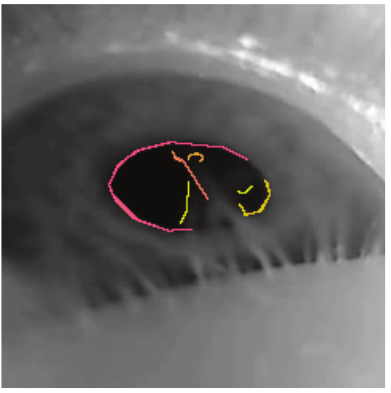
\includegraphics[width=.30\textwidth]{./Pictures/contours.png}
        }
   }
   \caption{Final Result of Extracting Contour module.
   \label{fig:Contours} }   
\end{dBox}   
\end{figure*}


\subsection{Extracting Contours} \index{Pupil Detection Algorithm}
	After getting the minimum edges we can extract Contours by using connected components, and then split the contours into sub-contours based on curvature continuity criteria as shown in Figure \ref{fig:Contours}. \cite{suzuki} \bigskip
	We have used OpenCV findCountours method to get all the contours from edges and then we get the approximate Poly-lines that each contour forms. So that, we can use each poly-line to get the angle between each subsequent 2 points to make sure that this contour is a good contour and also it helps to split contours into sub-contours based on angles between two subsequent points.  


\begin{figure*}[]
\begin{dBox}
\centering
  \mbox{
	    \subfigure[Final ellipse with center in red and supporting edge pixels are drawn in white.]{
	          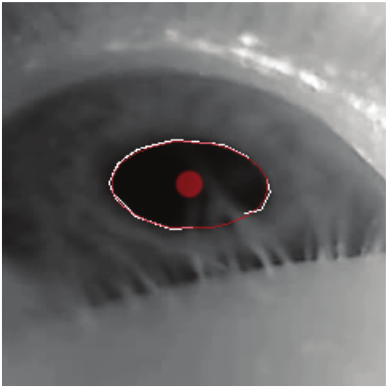
\includegraphics[width=.30\textwidth]{./Pictures/final_ellipse.png}
        }
   }
   \caption{Final Result of Ellipse Fitting module.
   \label{fig:EllipseFit} }   
\end{dBox}   
\end{figure*}


\subsection{Ellipse Fitting} \index{Pupil Detection Algorithm}
	Finally we should estimate the best ellipse that surrounds the Pupil by fitting an ellipse found through an augmented combinatorial search. \cite{fitzgibbon96} \bigskip
	
	Candidate pupil ellipses are formed using ellipse fitting onto a subset of the contours looking for good fits in a least square sense, major radii within a user defined range and a few additional criteria. An augmented combinatorial search looks for contours that can be added as support to the candidate ellipses. The results are evaluated based on the ellipse fit of the supporting edges and the ratio of supporting edge length and ellipse circumference. We call this ratio “ confidence ”. If the best results confidence is above a threshold the algorithm reports this candidate ellipse as the ellipse defining the contour of the pupil as shown in Figure \ref{fig:EllipseFit}. Otherwise the algorithm reports that no pupil was found. \bigskip
	
	
\section{Performance Evaluation} \index{Performance Evaluation}
	We have used Data Set of Computer Laboratory, University of Cambridge, United Kingdom which is used at Robust real-time pupil tracking in highly off-axis images to test performance. \cite{swirski} \\
	These Data Set contains video frames as individual images, and a text file describing the pupil ellipse in selected frames. The format of each line in text file is $<$frame \#$>$ $| <x> <y> <a> <b> < \theta >$, such that $ x , y$ represents the pupil center in frame\# , $ a, b$ represents the ellipse major radius and minor radius  values and $\theta$ represents angle between the major axis and the x-axis in radians. Total number of frames is 940 frame. \\
	Finally after Testing our implementation on this Data Set, we have make a comparison between our results and the original pupil center location. So we found the Average error = 1.545478. You Can see the 	Error graph in Figure \ref{fig:ErrorGraph}.
		

\begin{figure*}[]
\begin{dBox}
\centering
  \mbox{
	    \subfigure[]{
	          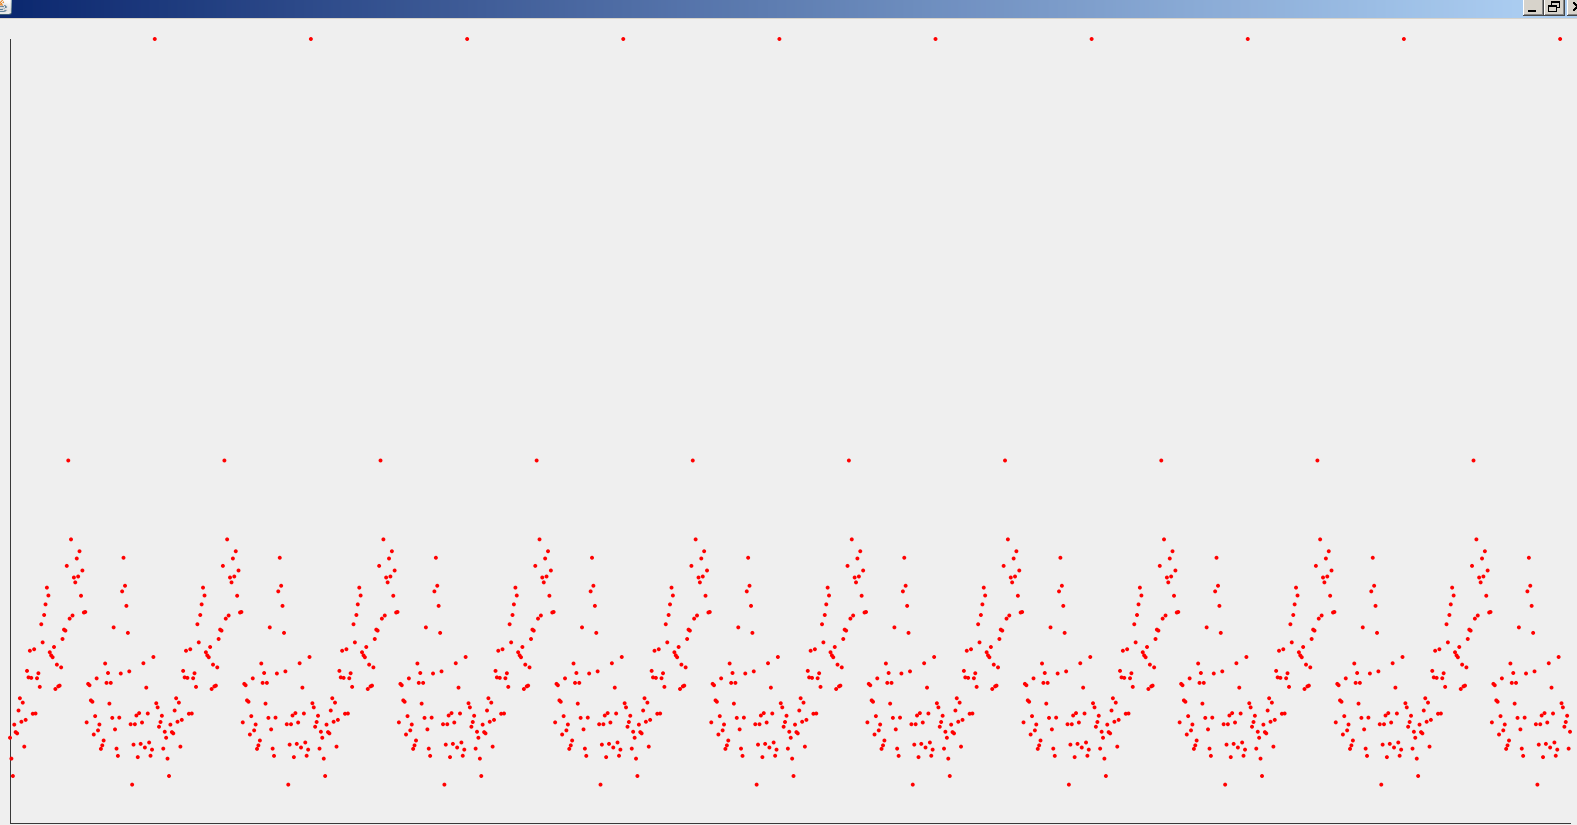
\includegraphics[width=.80\textwidth]{./Pictures/ErrorGraph.png}
        }
   }
   \caption{Error graph for Pupil algorithm performance test
   \label{fig:ErrorGraph} }   
\end{dBox}   
\end{figure*}
 

%----------------------------------------------------------------------------------------
%	CHAPTER 4  MIRT Eye Tracking Algorithm
%----------------------------------------------------------------------------------------
\chapterimage{eyes_women_cropped.jpg}
\chapter{MIRT} \index{MIRT}
In this chapter we present MIRT: Morphological Based Iris Tracking a novel method for real-time iris detection and tracking. MIRT is a morphological based real-time iris detection algorithm. Morphological operations are simple and fast to compute which reduces the time required to detect the iris. 

Two typed of image processing in eye tracking are used; visible and infrared spectrum imaging. Most available eye tracking approaches like Starburst \cite{starburst} and Pupil \cite{pupil} rely on infrared spectrum imaging. It's known that visible spectrum imaging is more complicated due to the uncontrolled ambient light that is used as a light source which usually contains multiple specular and diffuse components. On the other hand infrared imaging eliminates uncontrolled specular reflection by illuminating the eye with a uniform and controlled infrared light \cite{starburst}. However, infrared imaging requires using special hardware (infrared cameras, infrared lights). MIRT uses visible imaging to track the iris. Not to mention that MIRT can be used outdoors which is not available using infrared based eye-tracking algorithms We also doesn't require any special hardware, we use a low resolution web-cam. Used hardware and head-mounted tracker will be discussed later in this book.\bigskip


\section{Overview}\index{Overview}
MIRT algorithm can be divided into 2 stages; 1) locating region of interest in the given image, and 2) detecting the iris in the region of interest located in stage 1. At first we transform the input frame to gray scale then we locate the parts of the visible parts of the sclera. Next we estimate the location of the iris based on the location of the sclera, and we crop the region of interest (ROI) from the source image. We try to minimize the ROI as possible to cut down the runtime and to minimize the error of the estimated iris center. From the extracted ROI we find the a set of feature points. An inlier feature points is a point that lies on the edge of the iris. Extracted feature points may contain some outliers, therefore we use RANSAC ellipse fitting to fit ellipse model on the extracted feature points. RANSAC is an effective technique for model fitting in the presence of a large but unknown percentage of outliers in a measurement sample. Using the RANSAC technique increase the ability of the system to do robust estimation of the model (ellipse) parameters. Figure \ref{fig:mirt_overview} shows the stages of the MIRT algorithm.

\begin{figure*}[!h]
\begin{dBox}
\centering
	\mbox{
		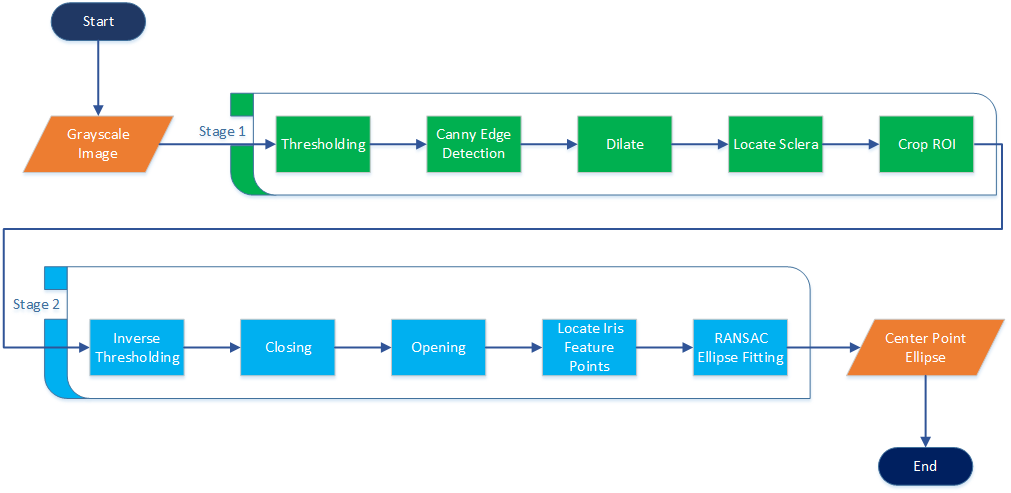
\includegraphics[width=\textwidth]{./Pictures/mirt/MIRT_overview.png}
	}
   \caption{Overview of MIRT Algorithm \label{fig:mirt_overview} }   
\end{dBox}   
\end{figure*}


\section{ROI Localization}\index{ROI Localization}
As figure \ref{fig:mirt_overview} illustrates the pipeline of the ROI localization step. We use simple thresholding on the input gray scale image (frame). Then we apply Canny edge detection algorithm \cite{canny} on the binary image. Then we dilate using a small structuring element just to fill the small gaps between edges and make edges wider. This goal from the dilation step is to increase the robustness of contour finding step. We use circular shaped small structuring element with diameter $ d = 3 $ pixels. \bigskip

The next stage is that we find the largest 2 contours that satisfy the size constrain. We defined a size threshold to eliminate the regions that might be mistaken with the sclera. When the iris is in the middle of limbus (corneal limbus is the border of the cornea and the sclera) 2 parts of the sclera are visible as illustrated in figure \ref{fig:roi_2p}. In this case the largest 2 contours will be two parts of the sclera and the iris is estimated to lie between those two parts. The ROI is set to be the bounding box of the two contours, shown in figure \ref{fig:roi_2p}. \bigskip

\begin{figure*}[!h]
\begin{dBox}
	\mbox{
	\centering
		\subfigure[Input image]{
			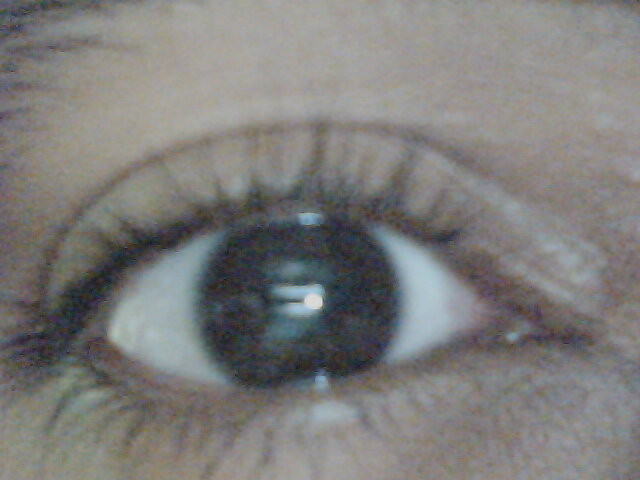
\includegraphics[width=.31\textwidth]{./Pictures/mirt/3.jpg}
			\label{fig:input_2p}
        }
        \subfigure[Illustration of stage 1]{
			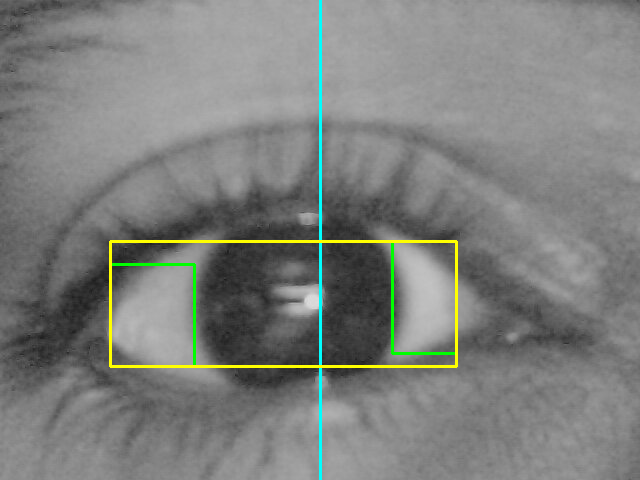
\includegraphics[width=.31\textwidth]{./Pictures/mirt/locate_roi_2p.png}
			\label{fig:roi_2p}
        }
        \subfigure[Algorithm output]{
			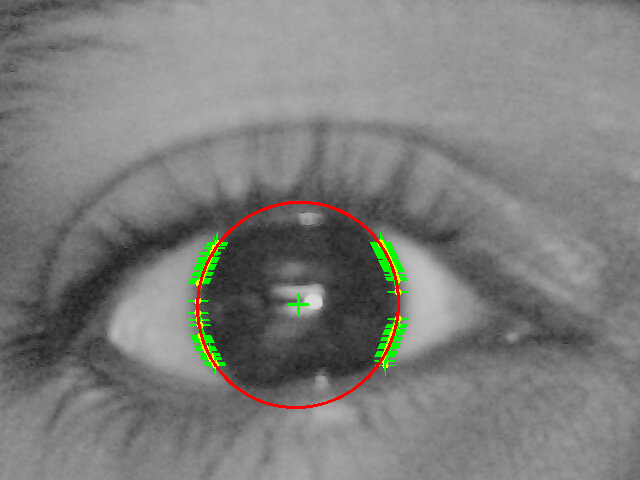
\includegraphics[width=.31\textwidth]{./Pictures/mirt/result_2p.png}
			\label{fig:result_2p}
        }
	}
   \caption{MIRT in action when 2 parts of sclera are visible; (a) shows the input image. (b) shows the 2 parts of sclera marked with green, ROI marked with yellow, and previous estimation of pupil center x with cyan. (c) shows the estimated ellipse with red and feature points with green cross-hairs. \label{fig:mirt_2p} }      
\end{dBox}   
\end{figure*}



\begin{figure*}[!h]
\begin{dBox}
	\mbox{
		
		\centering
		\subfigure[Input image]{
			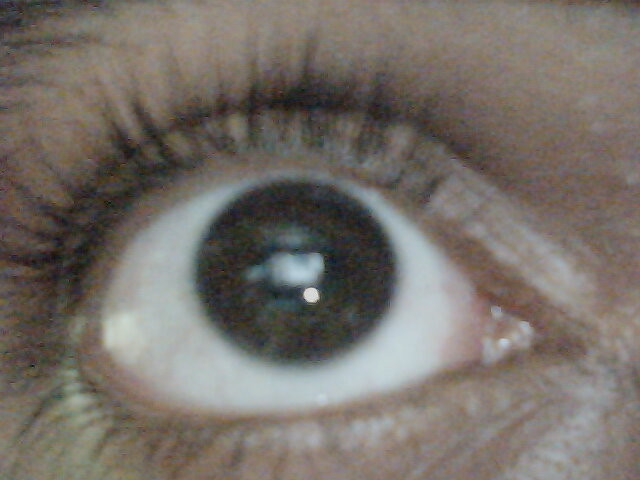
\includegraphics[width=.31\textwidth]{./Pictures/mirt/4.jpg}
			\label{fig:input_1p}
        }
        \subfigure[Illustration of stage 1]{
			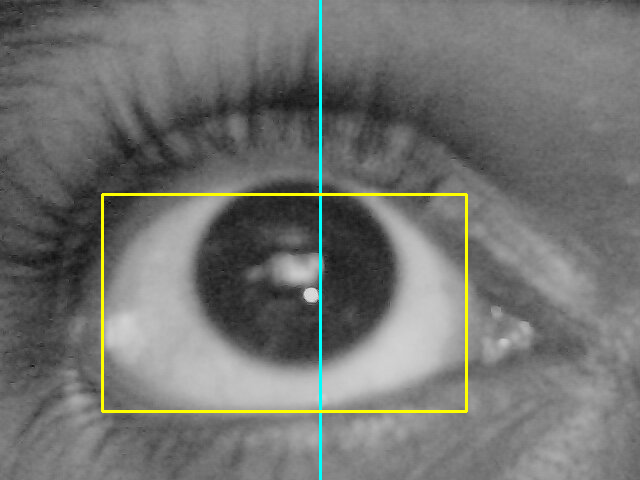
\includegraphics[width=.31\textwidth]{./Pictures/mirt/locate_roi_1p.png}
			\label{fig:roi_1p}
        }
        \subfigure[Algorithm output]{
			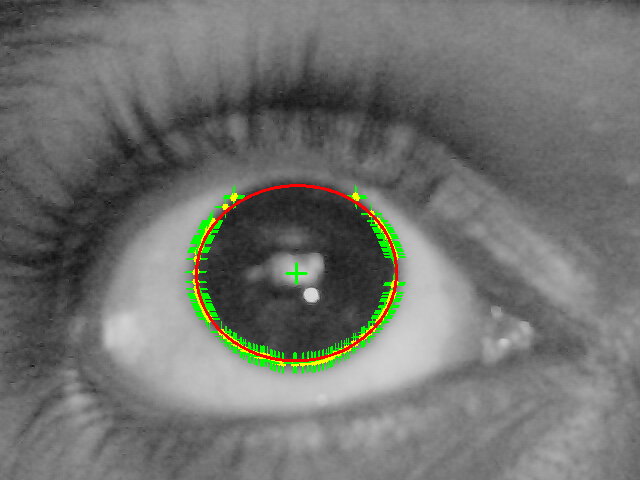
\includegraphics[width=.31\textwidth]{./Pictures/mirt/result_1p.png}
			\label{fig:res_1p}
        } 
    }
\caption{MIRT in action when 2 connected parts of sclera are visible; (a) shows the input image. (b) shows the visible contour of sclera marked with green, ROI marked with yellow, and previous estimation of pupil center x with cyan. (c) shows the estimated ellipse with red and feature points with green cross-hairs. \label{fig:mirt_1p} }      
\end{dBox}
\end{figure*}

In other cases when the iris is either on the left or on the right of the limbus, only one part of the sclera is visible which is the largest contour found in the image, hence we have 3 different situations. If the width of the largest contour is greater than twice the estimated iris size $ h = 150 $ (based on our head mounted camera) then the ROI is the bounding rectangle of the largest contour as illustrated in figure \ref{fig:mirt_1p}. We assume that the iris is nearly at the center of the limbus, yet one of the visible sclera contours couldn't be extracted. \bigskip

% TODO ensure this part is on the same page
For the two other cases we define a placement ratio 
	\begin{dBox}
		\centering
		$$ r = abs ( \frac{ c - x_{start}}{x_{end} - c } ) $$
	\end{dBox}
where $c$ is the x coordinate value of the iris center estimated in the previous frame, $c$ is set to the center of the image in the first frame. $x_{start}$ and $x_{end}$ are the x coordinates of the start and the end of largest contour. In other words $r$ is the ratio between the both sides of the largest contours to the initial center of the pupil. If $r \leq 1 $ then the iris is on the right and the left part of the sclera is visible. The ROI width stretches from $x_{end} - h/2$ to $x_{end} + h $ and have the same hight of the largest. See figure \ref{fig:mirt_l} for illustration. \bigskip

\begin{figure*}[!h]
\begin{dBox}
	\mbox{

        \subfigure[Input image]{
			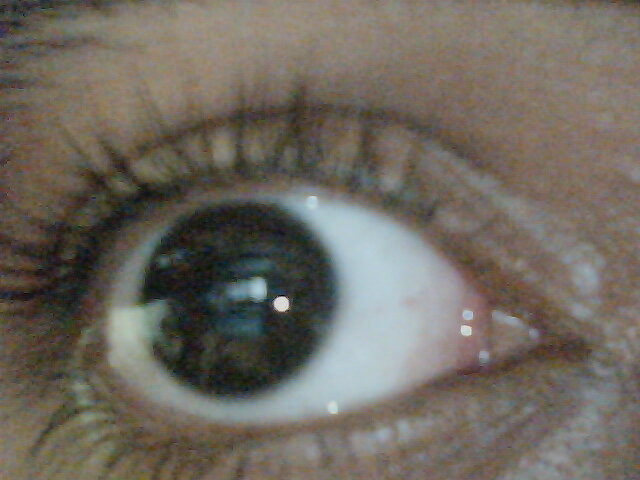
\includegraphics[width=.31\textwidth]{./Pictures/mirt/2.jpg}
			\label{fig:input_l}
        }
        \subfigure[Illustration of stage 1]{
			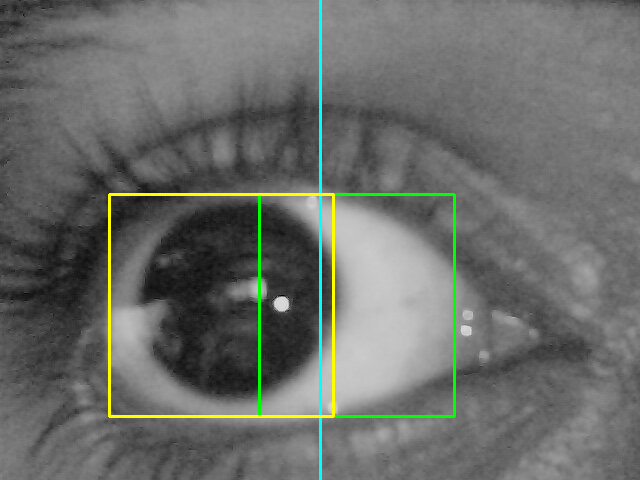
\includegraphics[width=.31\textwidth]{./Pictures/mirt/locate_roi_l.png}
			\label{fig:roi_l}
        }
        \subfigure[Algorithm output]{
			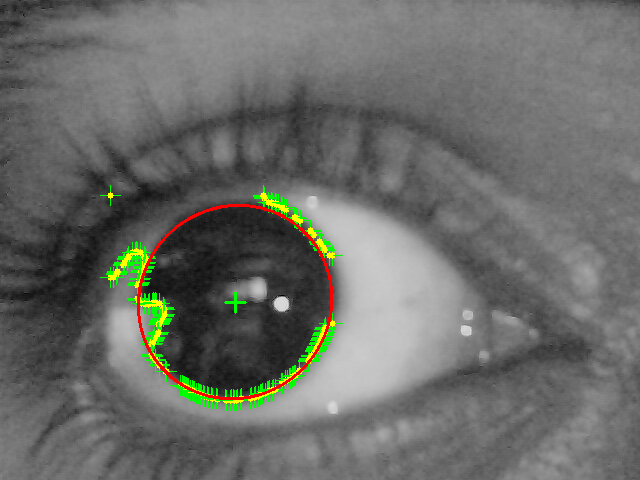
\includegraphics[width=.31\textwidth]{./Pictures/mirt/result_l.png}
			\label{fig:res_l}
        } 
    }|    
\caption{MIRT in action when the right side of sclera is visible; (a) shows the input image. (b) shows the visible (right) side of sclera marked with green, ROI marked with yellow, and previous estimation of pupil center x with cyan. (c) shows the estimated ellipse with red and feature points with green cross-hairs. \label{fig:mirt_l} }      
\end{dBox}
\end{figure*}

The opposite case is that if $r > 1$ then the iris is in the left and the right part of the sclera is visible. Similar to the previous case the ROI is set to be $x_{start} - h$ to $x_{start} + h/2 $ in width and also have the same height of the largest contour. Figure \ref{fig:mirt_r} shows this case. One last case remaining is that none of the found contours satisfied the size condition, this situation can occur in frames where the limbus is not visible (i.e blink), hence the frame is skipped. Finally if the estimated bounds of the ROI are outside input image boundaries the ROI boundaries are clamped to the input image bounds. Algorithm \ref{mirt_roi_loc_algo} illustrates the procedure of MIRT ROI localization stage.

\begin{figure*}[!h]
\begin{dBox}
	\mbox{

        \subfigure[Input image]{
			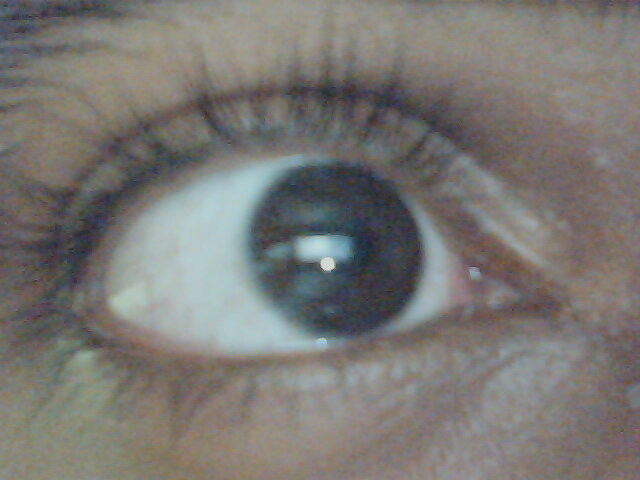
\includegraphics[width=.31\textwidth]{./Pictures/mirt/1.jpg}
			\label{fig:input_r}
        }
        \subfigure[Illustration of stage 1]{
			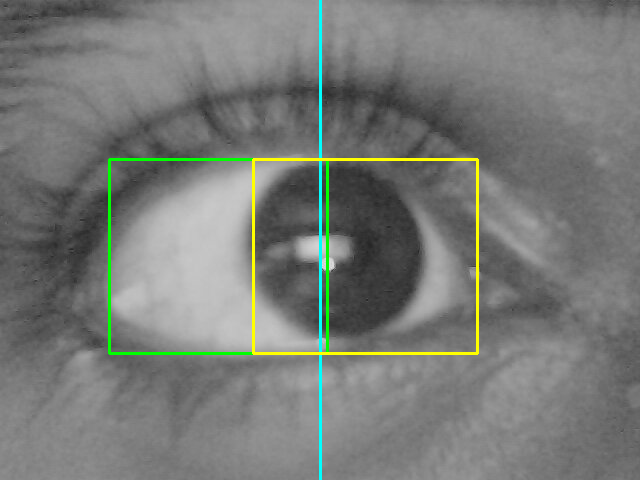
\includegraphics[width=.31\textwidth]{./Pictures/mirt/locate_roi_r.png}
			\label{fig:roi_r}
        }
        \subfigure[Algorithm output]{
			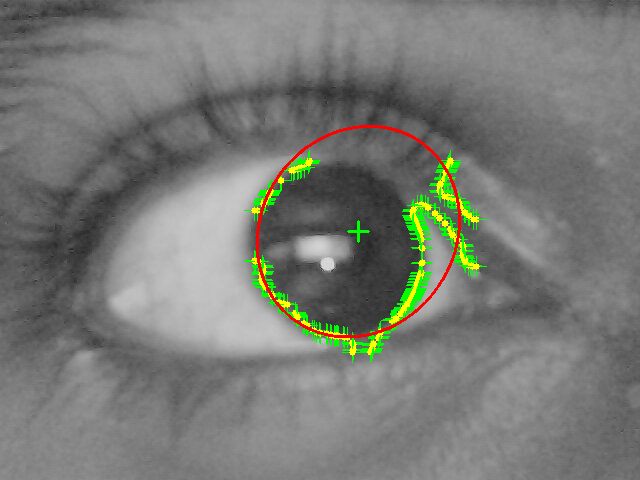
\includegraphics[width=.31\textwidth]{./Pictures/mirt/result_r.png}
			\label{fig:res_r}
        } 
	}

\caption{MIRT in action when the left side of sclera is visible; (a) shows the input image. (b) shows the visible (left) side of sclera marked with green, ROI marked with yellow, and previous estimation of pupil center x with cyan. (c) shows the estimated ellipse with red and feature points with green cross-hairs. \label{fig:mirt_r} }      
\end{dBox}
\end{figure*}

\begin{algorithm}[!h]
\begin{dBox}

	\caption{MIRT: Locate ROI (Stage 1)} \label{mirt_roi_loc_algo}
	\begin{algorithmic}[1]
		\Require{grayscale eye image}
		\Ensure {grayscale ROI image}
		\Procedure{MIRT: locate ROI}{}
		\State $binary \gets$ \Call{threshold}{$input$}
		\State $edges \gets$ \Call{canny}{$binary$}
		\State \Call{dilate}{$edges$}
		\State $largest,\: secondlargest \gets$ \Call{findContours}{$edges$}

		\If{\Call{area}{largest} < $AREA\_THRES$} \Comment{no valid contours found}
			\State terminate
		\ElsIf{\Call{area}{$secondlargest$} < $AREA\_THRES$}  \Comment{only 1 contour found}
			\State $c \gets previous\_center.x$
			\State $r \gets (c-x_{start})/(x_{end}-c)$

			\If{$largest.width > 2*IRIS\_SIZE$}
				\State $ROI \gets$ \Call{rectangle}{$largest$}
			\ElsIf{$r < 1$}	\Comment{right part visible}
				\State $ROI.x_{start} \gets largest.x_{start} - IRIS\_SIZE $
				\State $ROI.x_{end} \gets largest.x_{start} + IRIS\_SIZE/2$
			\Else  \Comment{left part visible}
				\State $ROI.x_{start} \gets largest.x_{end} - IRIS\_SIZE/2 $
				\State $ROI.x_{start} \gets largest.x_{end} + IRIS\_SIZE$
			\EndIf

		\Else  
			\Comment{2 contour found}
			\State $ROI \gets $\Call{boundingrectangle}{$largest, \: secondlargest$}
		\EndIf

		\Call{crop}{$input, \: ROI$} 
		\Comment{crop the input image to the ROI}
		
		\Return $ROI$
		\EndProcedure	
	\end{algorithmic}
\end{dBox}	
\end{algorithm}



\section{Locate Iris In ROI} \index{Locate Iris In ROI}
In this stage we are interested in finding the iris in the tightly cropped ROI located in stage 1. we start by applying inverse simple thresholding to filter dark areas in the ROI. Next we apply morphological closing followed by opening using 19 pixel circular structuring element. The main goal of this step to fill the gaps in the iris (gaps come from light reflections) and to open between the iris and other parts of the ROI that passed through the thresholding step. Then we find the largest contour in the ROI. In almost all cases the largest contour will contain the iris as shown in figure \ref{fig:iris_contour}. Finally we extract feature points from the largest contour. Edge points of the contour are considered as feature points. We use Random Sample Consensus (RANSAC) paradigm for model fitting \cite{ransac}. RANSAC is an effective technique for model fitting in the presence of a large but unknown percentage of outliers in a measurement sample. In our application inliers are feature points that lie on the iris contour, while outliers are feature points that belong to other contours other than the iris contour. Using the RANSAC technique increase the ability of the system to do robust estimation of the model (ellipse) parameters. We draw 5 samples from the detected feature set, then we compute the best fit ellipse using Fitzgibbon’s algorithm \cite{fitzgibbon96} which is implemented in OpenCV. Finally we evaluate the error between the estimated model and all feature points and count inliers / outliers. Algorithms \ref{mirt_iris_algo} and \ref{our_ransac} summarizes stage 2 procedure and how we use RANSAC in our system respectively. Figure \ref{fig:loc_iris} shows the steps of stage 2. 


\begin{figure}[!h]
\begin{dBox}
	
	\centering
	\mbox{
        \subfigure[Grayscale ROI]{
			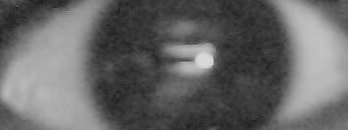
\includegraphics[width=.49\textwidth]{./Pictures/mirt/ROI.png}
			\label{fig:iris_roi}
        }

		\subfigure[Binary]{
			
\includegraphics[width=.49\textwidth]{./Pictures/mirt/binary.png}
			\label{fig:iris_binary}
        } 
    } 
    \mbox{
        \subfigure[Closing/Opening]{
			
\includegraphics[width=.49\textwidth]{./Pictures/mirt/morph.png}
			\label{fig:morph}
        }
        \subfigure[Largest Contour / Feature Points]{
			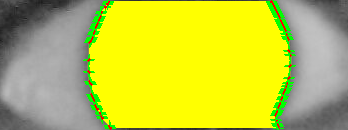
\includegraphics[width=.49\textwidth]{./Pictures/mirt/contour.png}
			\label{fig:iris_contour}
        } 
    }    
    \mbox{    
         \subfigure[Estimated Ellipse]{
			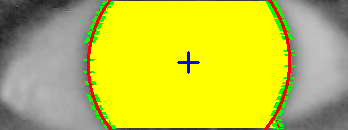
\includegraphics[width=.49\textwidth]{./Pictures/mirt/color_roi.png}
			\label{fig:iris_ellipse}
        } 
	}

\caption{Visualization of MIRT stage 2. (a) shows the input cropped ROI, (b) shows the binary image after inverse thresholding, (c) shows the binary image after performing closing followed by opening, (d) visualizes the largest contour in the image (colored with yellow) and extracted feature points marked with green cross-hairs and red points, (e) shows the estimated ellipse with red curve. \label{fig:loc_iris} }      
\end{dBox}
\end{figure}



\begin{algorithm}[!h]
\begin{dBox}
	\caption{MIRT: Locate Iris (Stage 2)} \label{mirt_iris_algo}
	\begin{algorithmic}[1]
		\Require{grayscale ROI image}
		\Ensure {Ellipse that describes the iris}
		\Procedure{MIRT: locate Iris}{}
		\State $binary \gets$ \Call{inversethreshold}{$input$}
		\State \Call{closing}{$binary$}
		\State \Call{opening}{$binary$}
		\State $largestcontour \gets$ \Call{findContours}{$binary$}
		\State $ellipse \gets$ \Call{RANSAC\_ellipse\_fitting}{$largestcontour$}
		\State \Return $ellipse$
		\EndProcedure	
	\end{algorithmic}
\end{dBox}	
\end{algorithm}


\begin{algorithm}
\begin{dBox}
	\caption{Our RANSAC Ellipse Fitting Procedure} \label{our_ransac}
	\begin{algorithmic}[1]
		\Procedure{RANSAC\_ellipse\_fitting}{}
		 \While{$i < N$}
			\State Draw $s$ points uniformly at random
			\State Fit ellipse model to these $s$ points
			\State Find inliers to this ellipse (points whose algebraic error $ < t$)
			\State If there are $d$ or more inliers, accept the ellipse and refit using all inliers	
		\EndWhile	
		\EndProcedure	
	\end{algorithmic}
\end{dBox}	
\end{algorithm}
 
%----------------------------------------------------------------------------------------
%	CHAPTER 5 // Eye Tracking Discussion and Evaluation
%----------------------------------------------------------------------------------------
\chapterimage{cover_4.png}
\chapter{Discussion and Evaluation} \index{Eye Tracking Discussion and Evaluation}

\section{Evaluation}\index{Evaluation}
In the previous chapters we discussed Starburst \cite{starburst}, Pupil \cite{pupil}, and MIRT eye tracking algorithms. Both Starburst and Pupil use infrared spectrum imaging. On the other hand MIRT is using visible spectrum imaging. Using visible spectrum is more complicated due to uncontrolled lighting conditions, which contain multiple specular and diffuse components. Capturing infrared images requires either using infrared cameras or using infrared lighting source with a traditional camera. For example \cite{scriptwear} describes  how to hack a traditional USB webcam to capture infrared images by removing the infrared filter and adding an infrared LED on camera chip. \bigskip

In MIRT we use visible spectrum which frees us from using special hardware. In visible spectrum images the corneal limbus (usually referred as limbus) is the strongest feature contour in the image, rather than the pupil which is the strongest feature contour when using infrared imaging. \bigskip

\begin{figure*}[!h]
\begin{dBox}
\centering
	\mbox{
		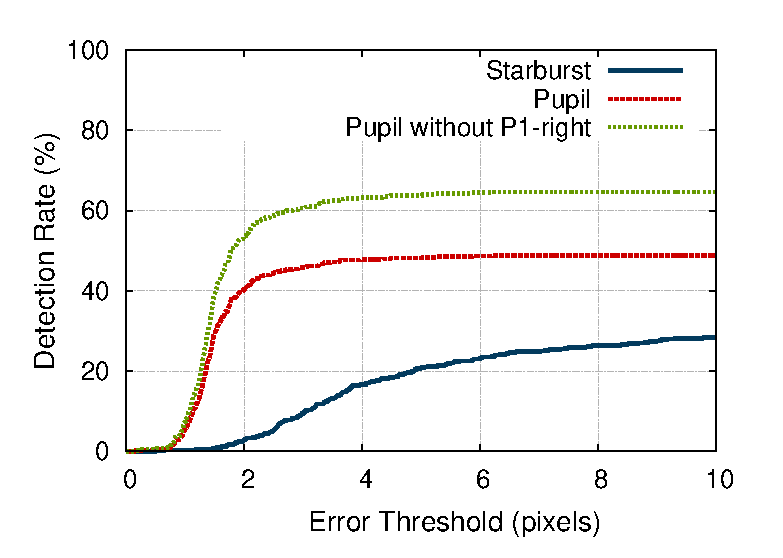
\includegraphics[width=\textwidth]{./Pictures/evaluation/error.eps}
	}
   \caption{Comparison of pupil detection rate between our implementation of Pupil algorithm and our implementation of Starburst algorithm using benchmark dataset by Swirski et al.\label{fig:our_eval} }   
\end{dBox}   
\end{figure*}

To evaluate our implementation of Starburst and Pupil we used the the benchmark dataset by Swirski et al. \cite{swirski}. Figure \ref{fig:our_eval} shows performance comparison between our implementation of Starburst described in chapter \ref{ch_starburst} and our implementation of Pupil algorithm \ref{ch_pupil}. As the figure indicates the performance of Starburst is relatively low compared to Pupil. The fall back in Starburst performance mainly results from the initial guess of the pupil center. A notable observation during the evaluation is that Starburst usually drops many frames until it detects the pupil, whenever the pupil is first is detected the detection rate in successive frames increase significantly. We tried to short circuit the Starburst initial estimate of pupil center (image center) with the actual pupil location I the first frame but the detection rate wasn't much affected. \bigskip

Moving to Pupil it can be clearly seen that Pupil overcomes Starburst. Pupil achieves about 48\% detection rate when evaluated using the complete dataset. If we exclude the dataset p1-right, that contains eye images recorded at the most extreme angles, the detection rate rise to 64\%. \bigskip

\begin{figure*}[!h]
\begin{dBox}
\centering
	\mbox{
		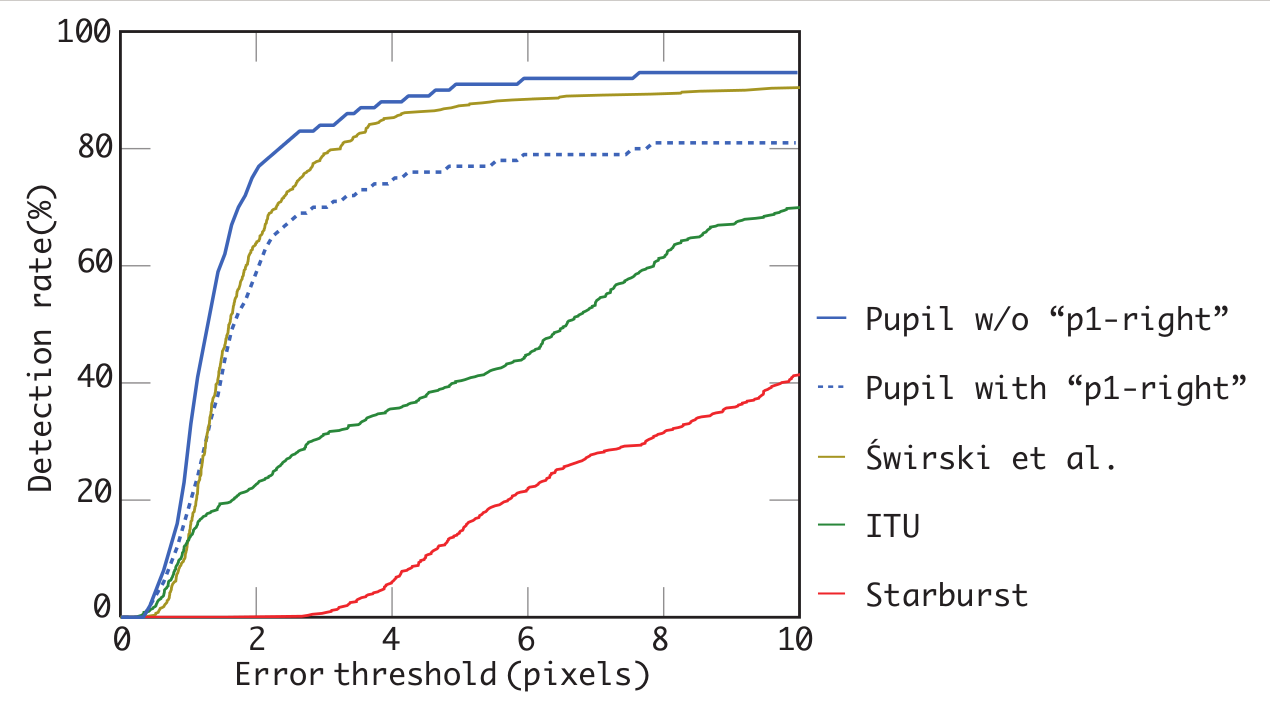
\includegraphics[width=\textwidth]{./Pictures/evaluation/comparison_pupil.png}
	}
   \caption{Comparison of pupil detection rate for Pupil’s algorithm, the stock algorithm proposed by Swirski et al., the ITU gaze tracker and Starburst. Figure from Pupil \cite{starburst} \label{fig:pupil_eval} }   
\end{dBox}   
\end{figure*}

Figure \ref{fig:pupil_eval} shows the evaluation on the same dataset mentioned in Pupil paper \cite{pupil} . This figure shows the performance difference between our implementation of Starburst and Pupil and actual implementations of both algorithms. Starburst we almost achieved the same performance level. On the other hand our implementation of pupil is about 20\% less accurate than the actual implementation.




\section{Headset Design and Hardware} \index{Headset Design and Hardware}
In our system we build a cheap (do it yourself - DIY) head mounded eye-tracker. Figure \ref{fig:headset} shows the prototype of our eye tracker. We used a traditional glasses frame after removing the lenses. Then we attached an internal laptop webcam to the frame. The webcam we used is a USB HP webcam. The chip comes with 2 integrated microphones, hence the camera chip has 6 pins while the USB has 4 wires. Correct pinout can be found at \cite{myblogpost}.



\begin{figure*}[!h]
\begin{dBox}
\centering
	\mbox{
		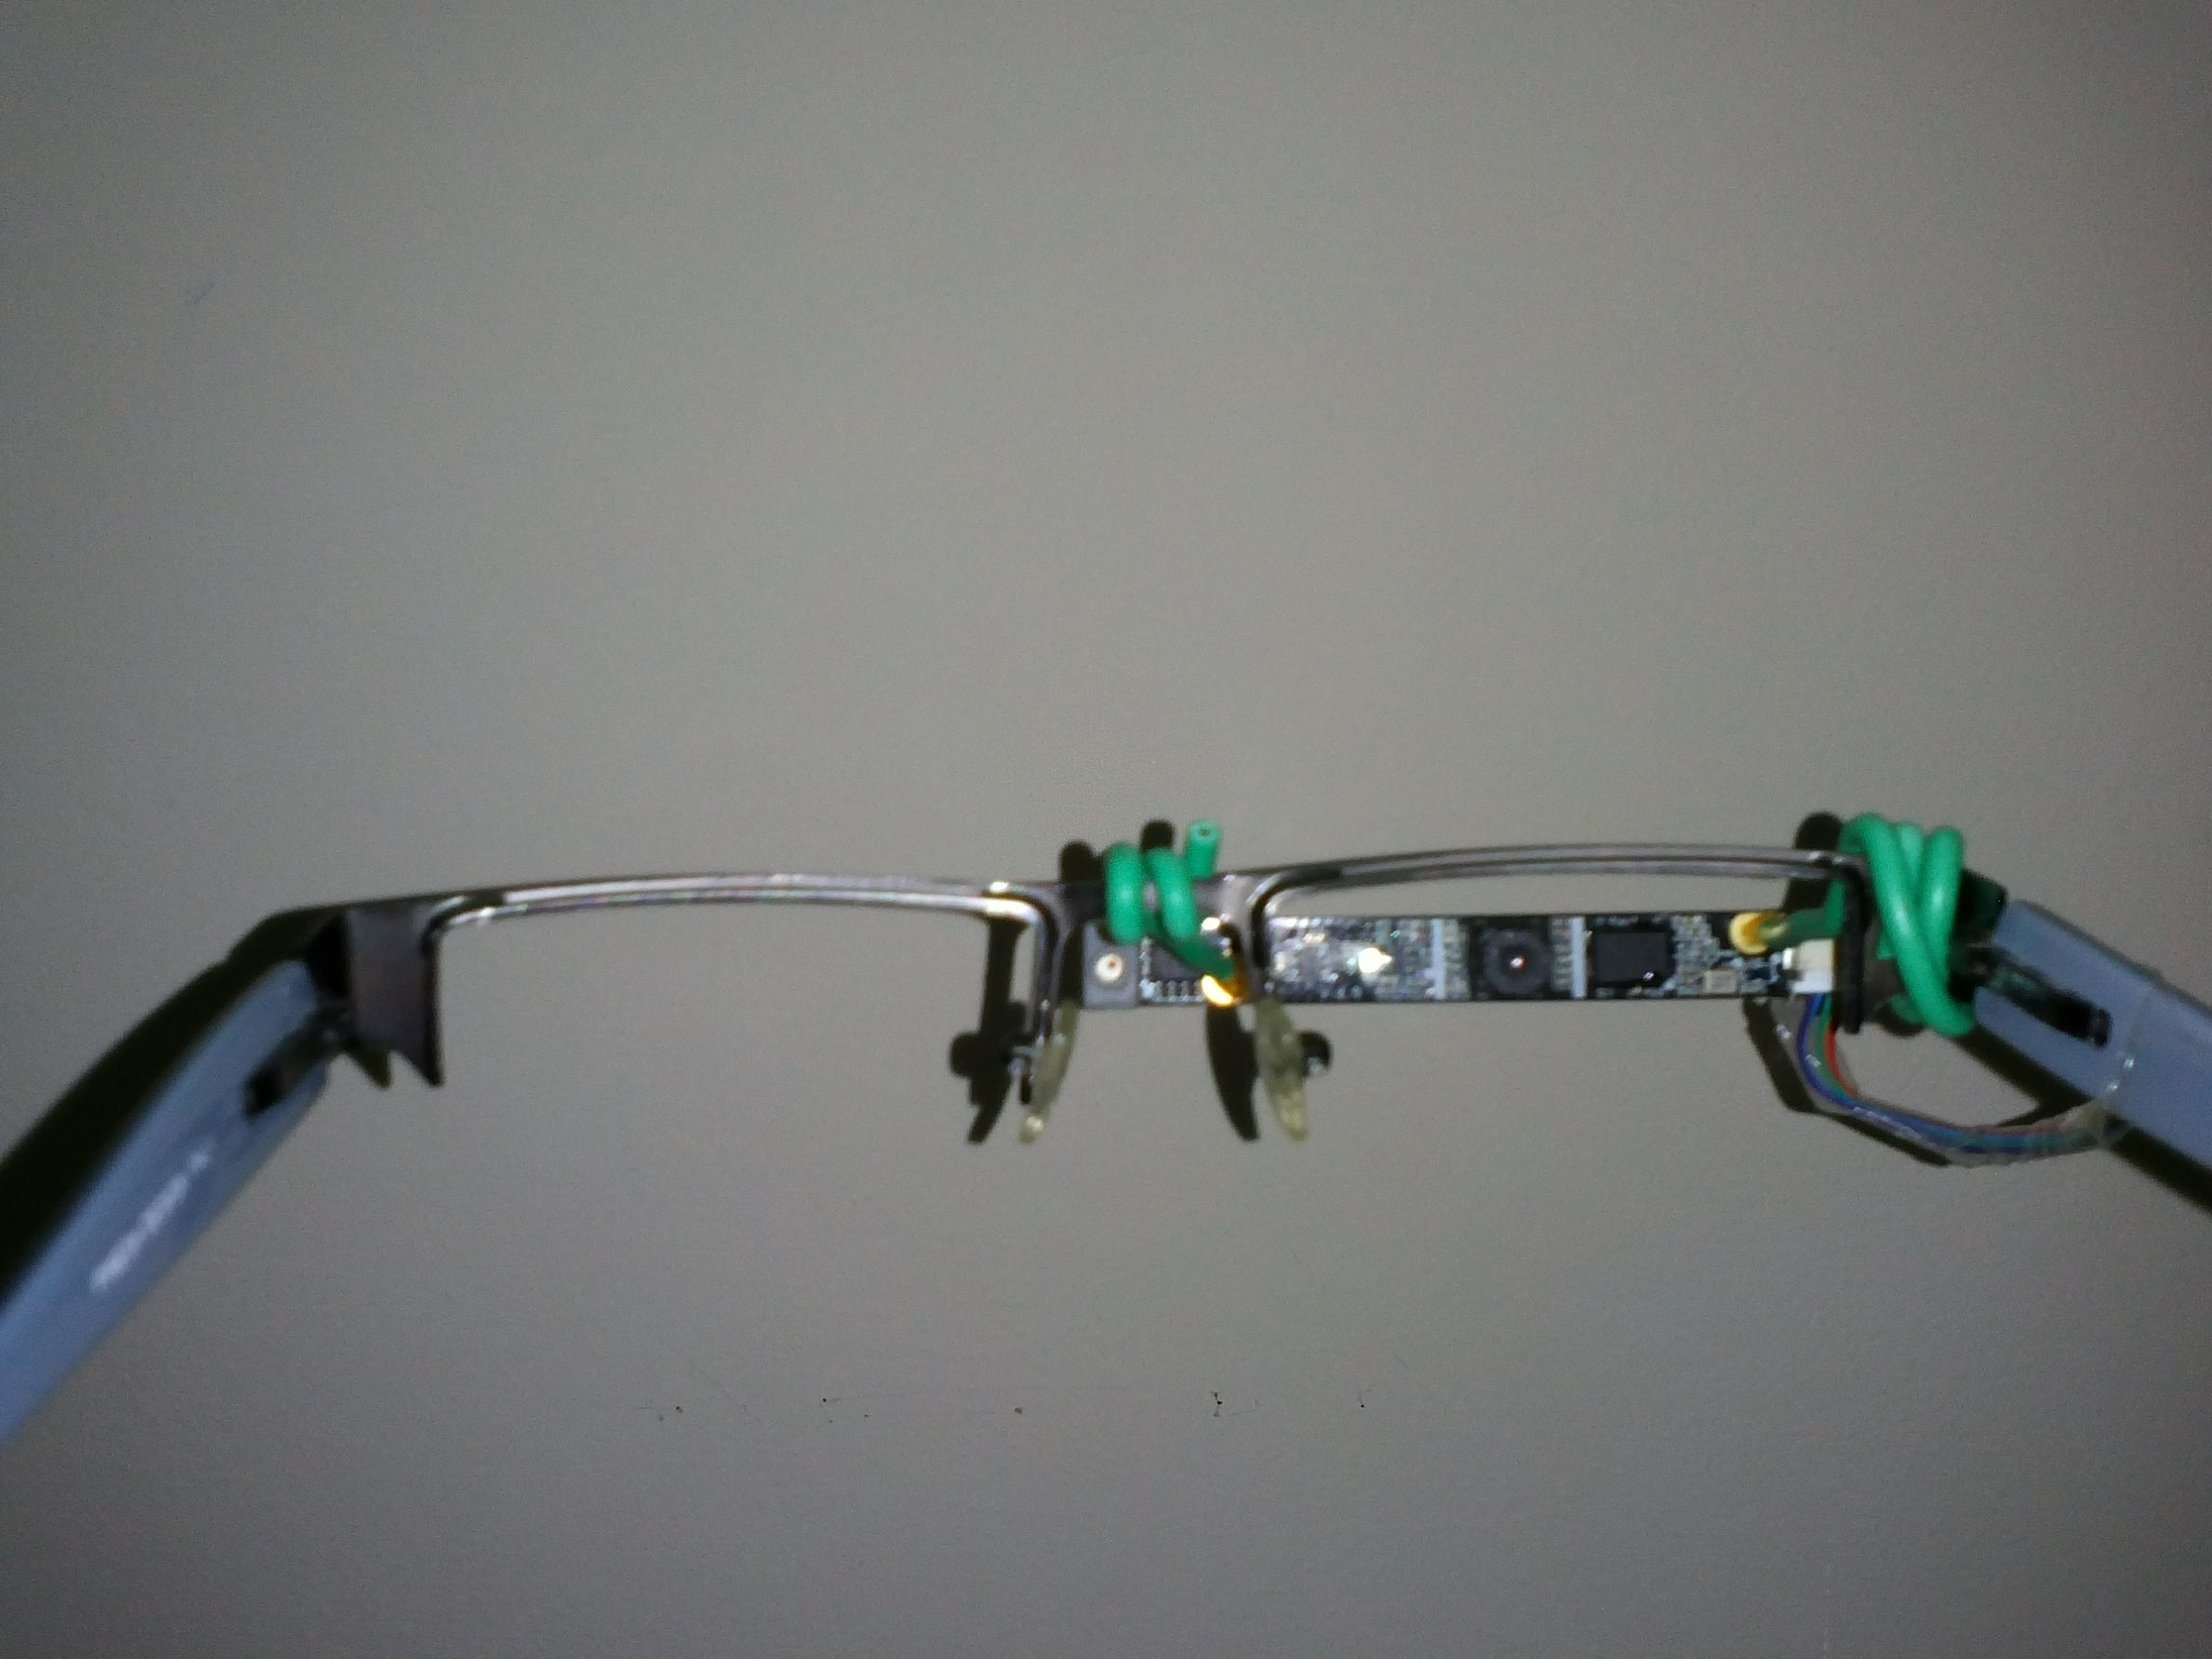
\includegraphics[width=.45\textwidth]{./Pictures/evaluation/cam_front.jpg}
		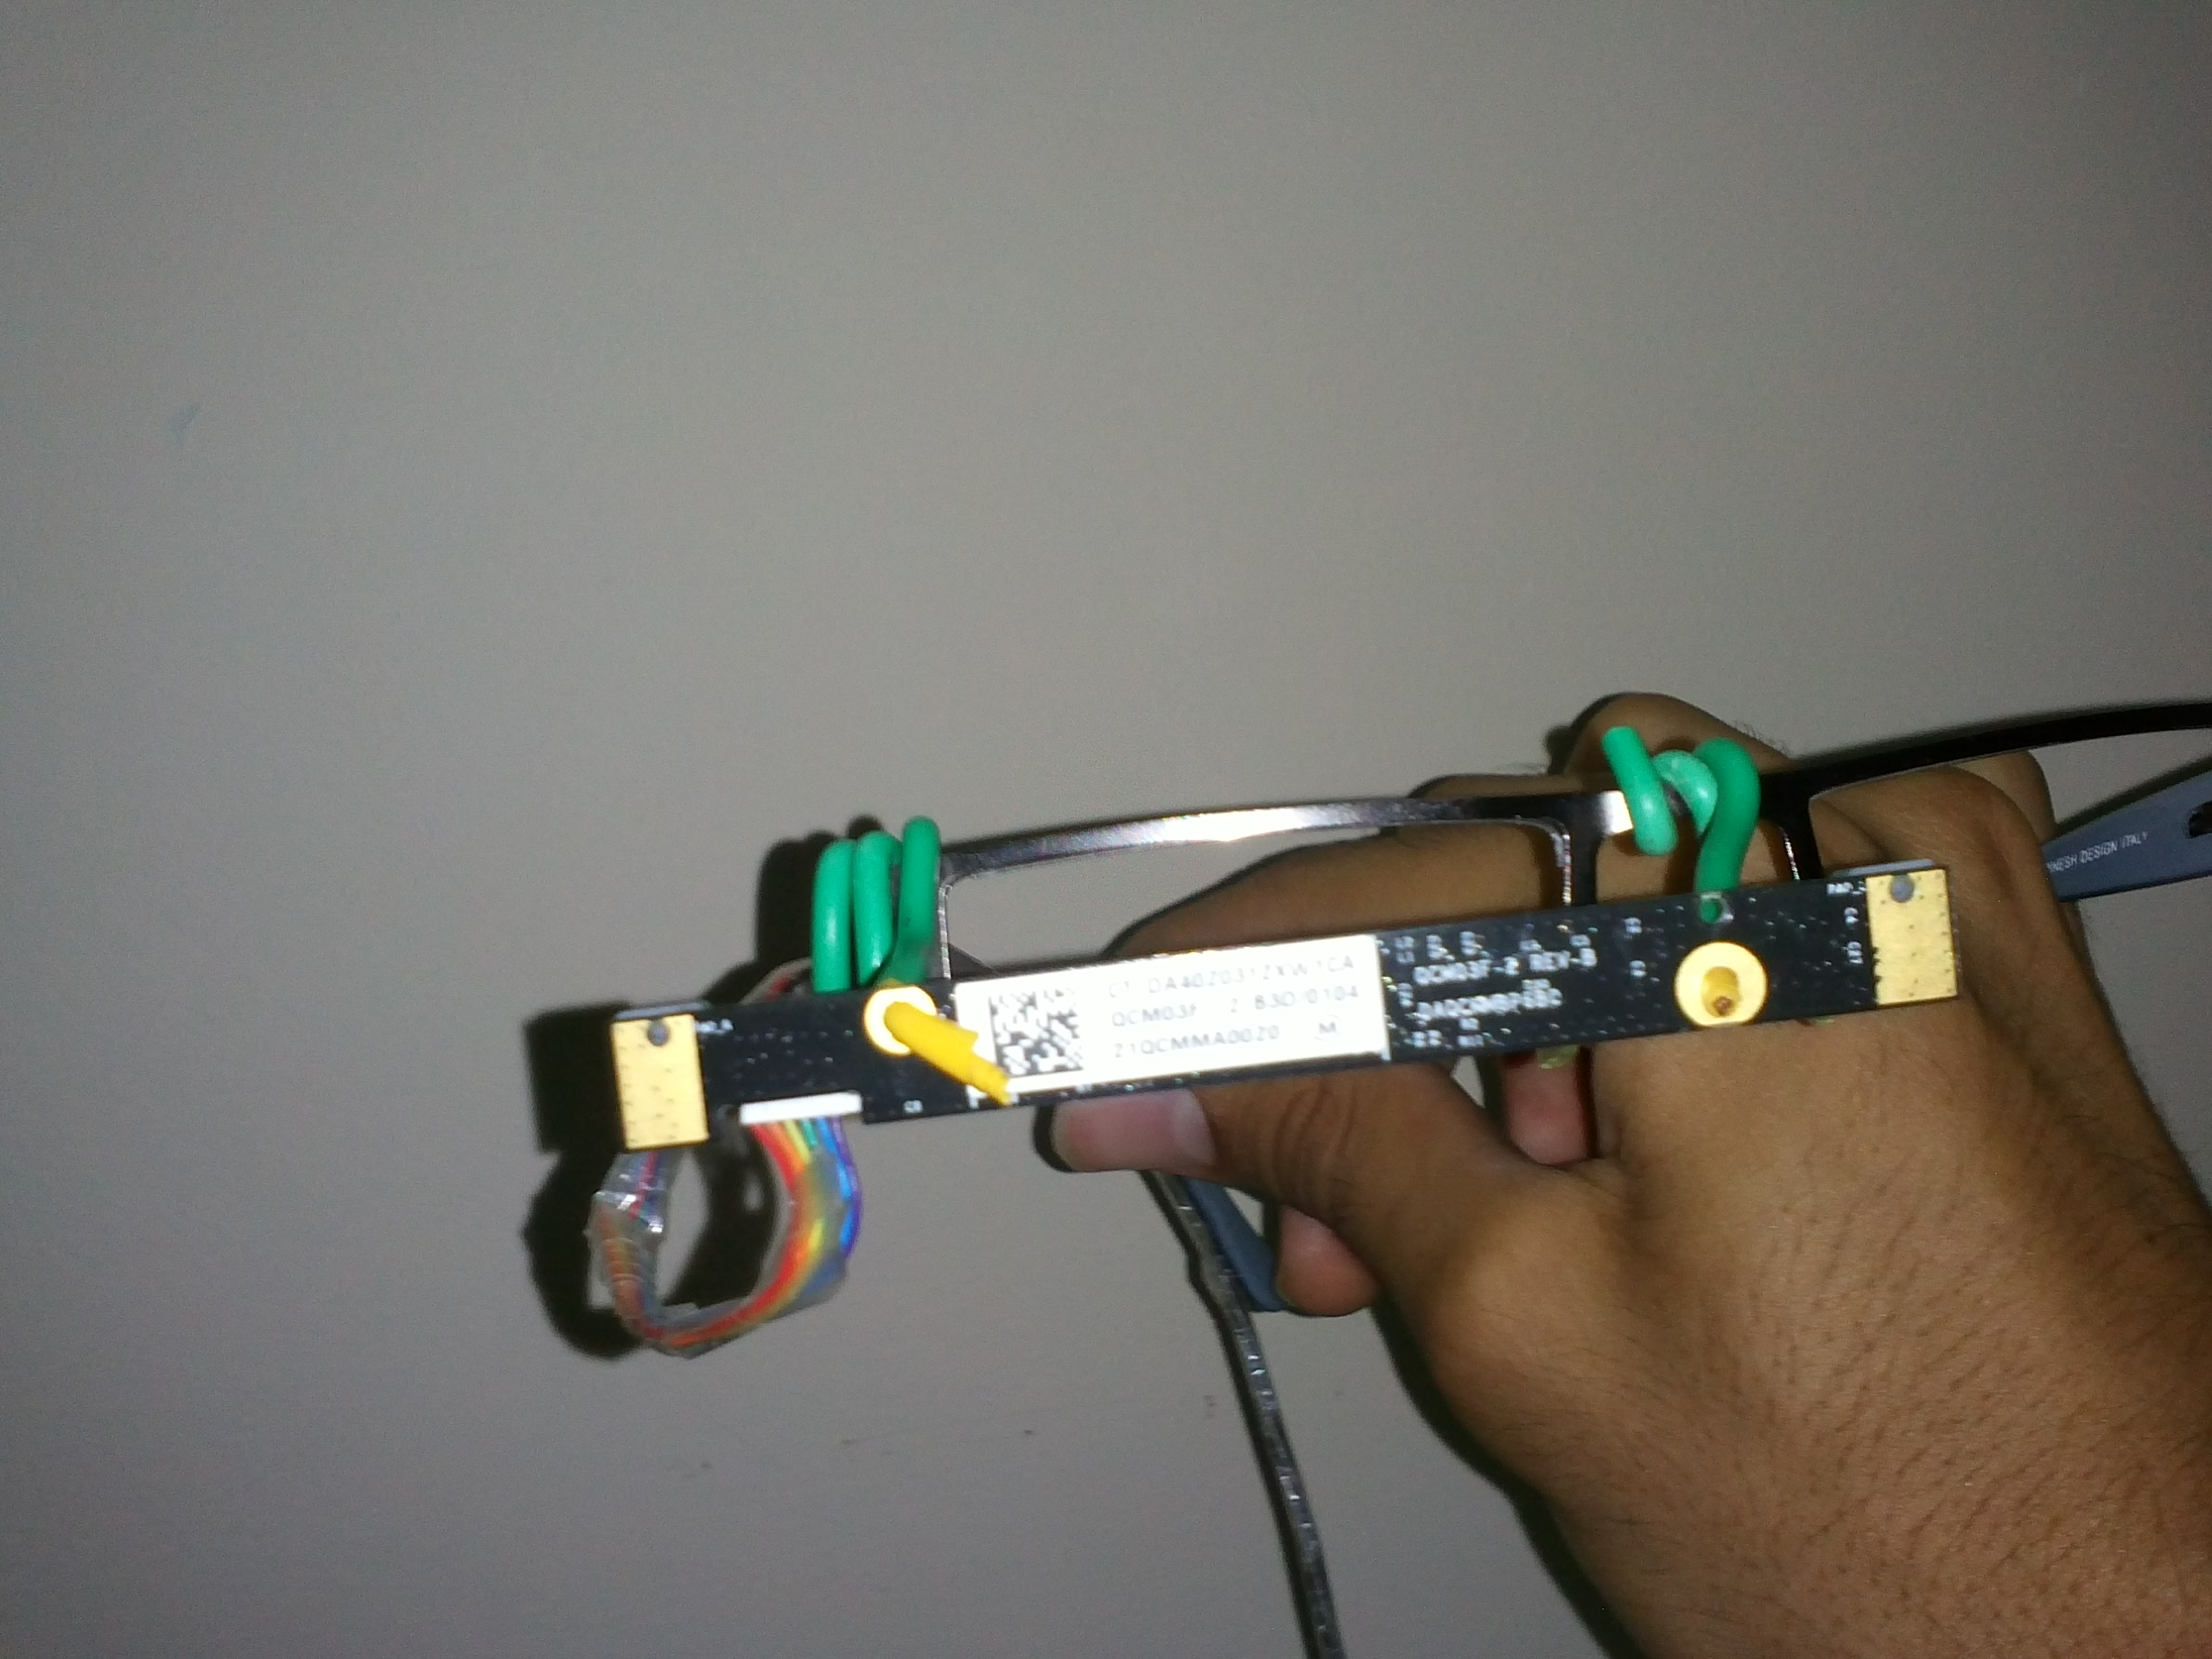
\includegraphics[width=.45\textwidth]{./Pictures/evaluation/cam_back.jpg}
	}
	\mbox{
		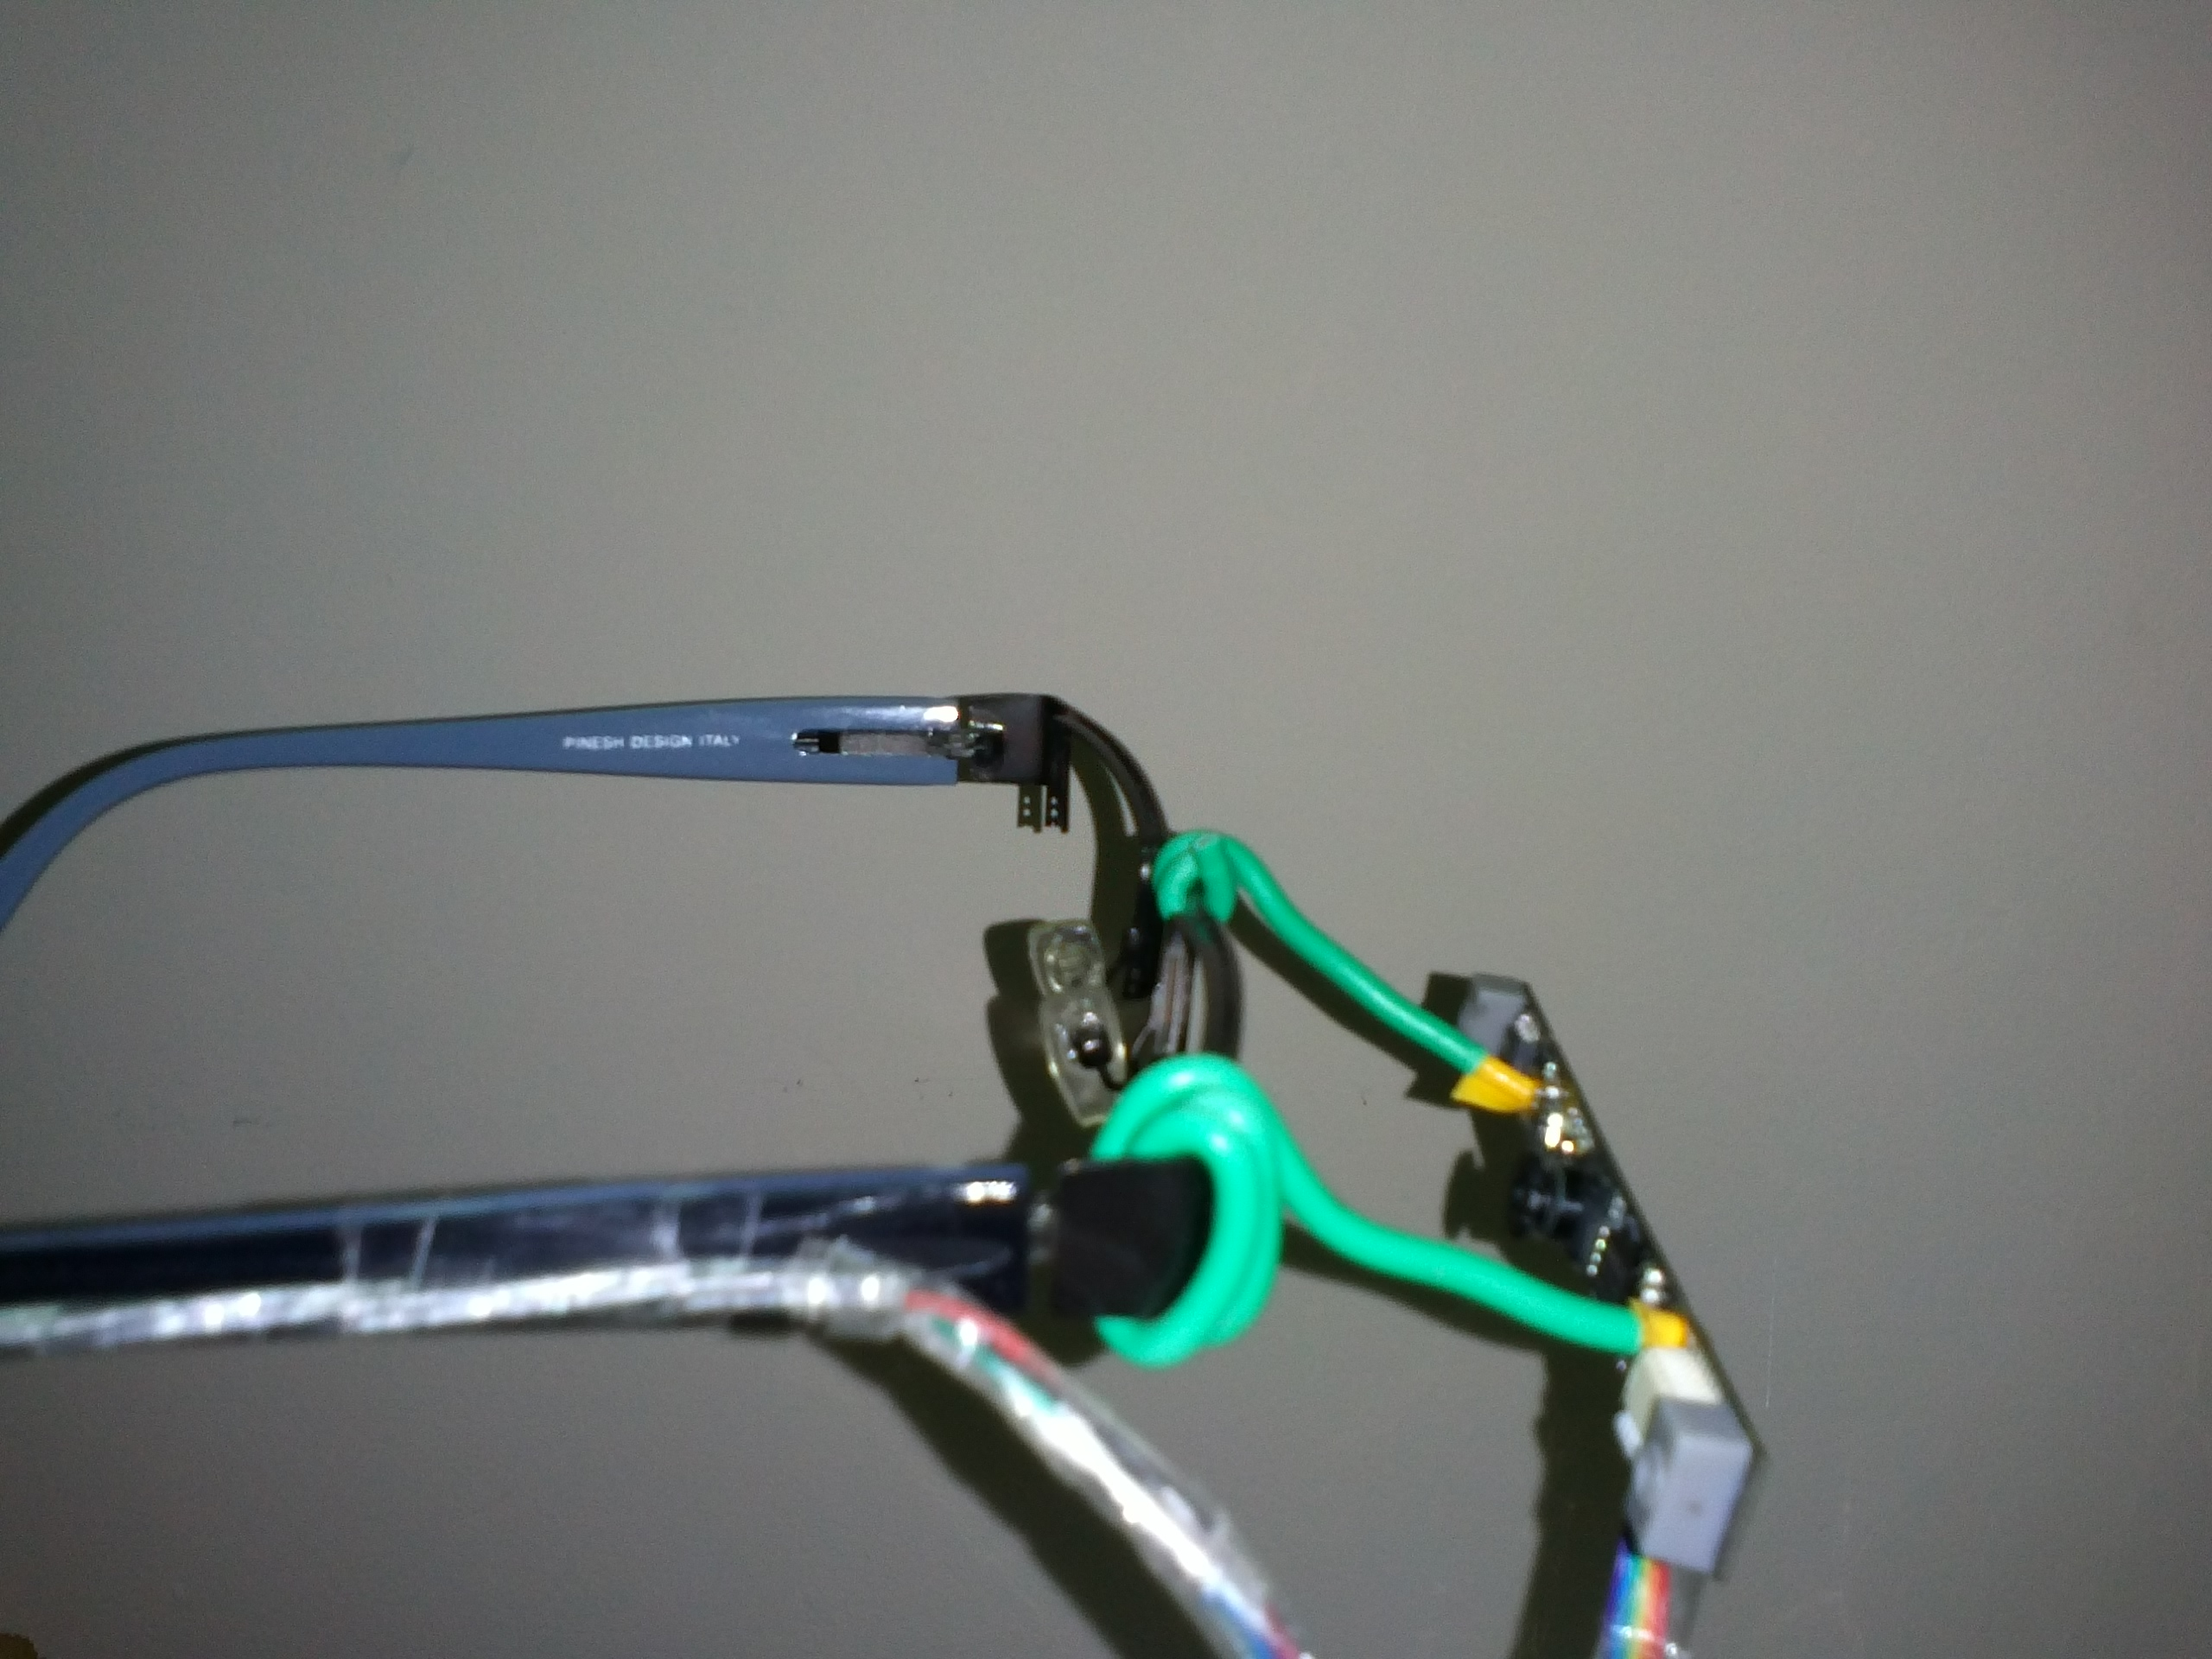
\includegraphics[width=.45\textwidth]{./Pictures/evaluation/cam_side.jpg}
		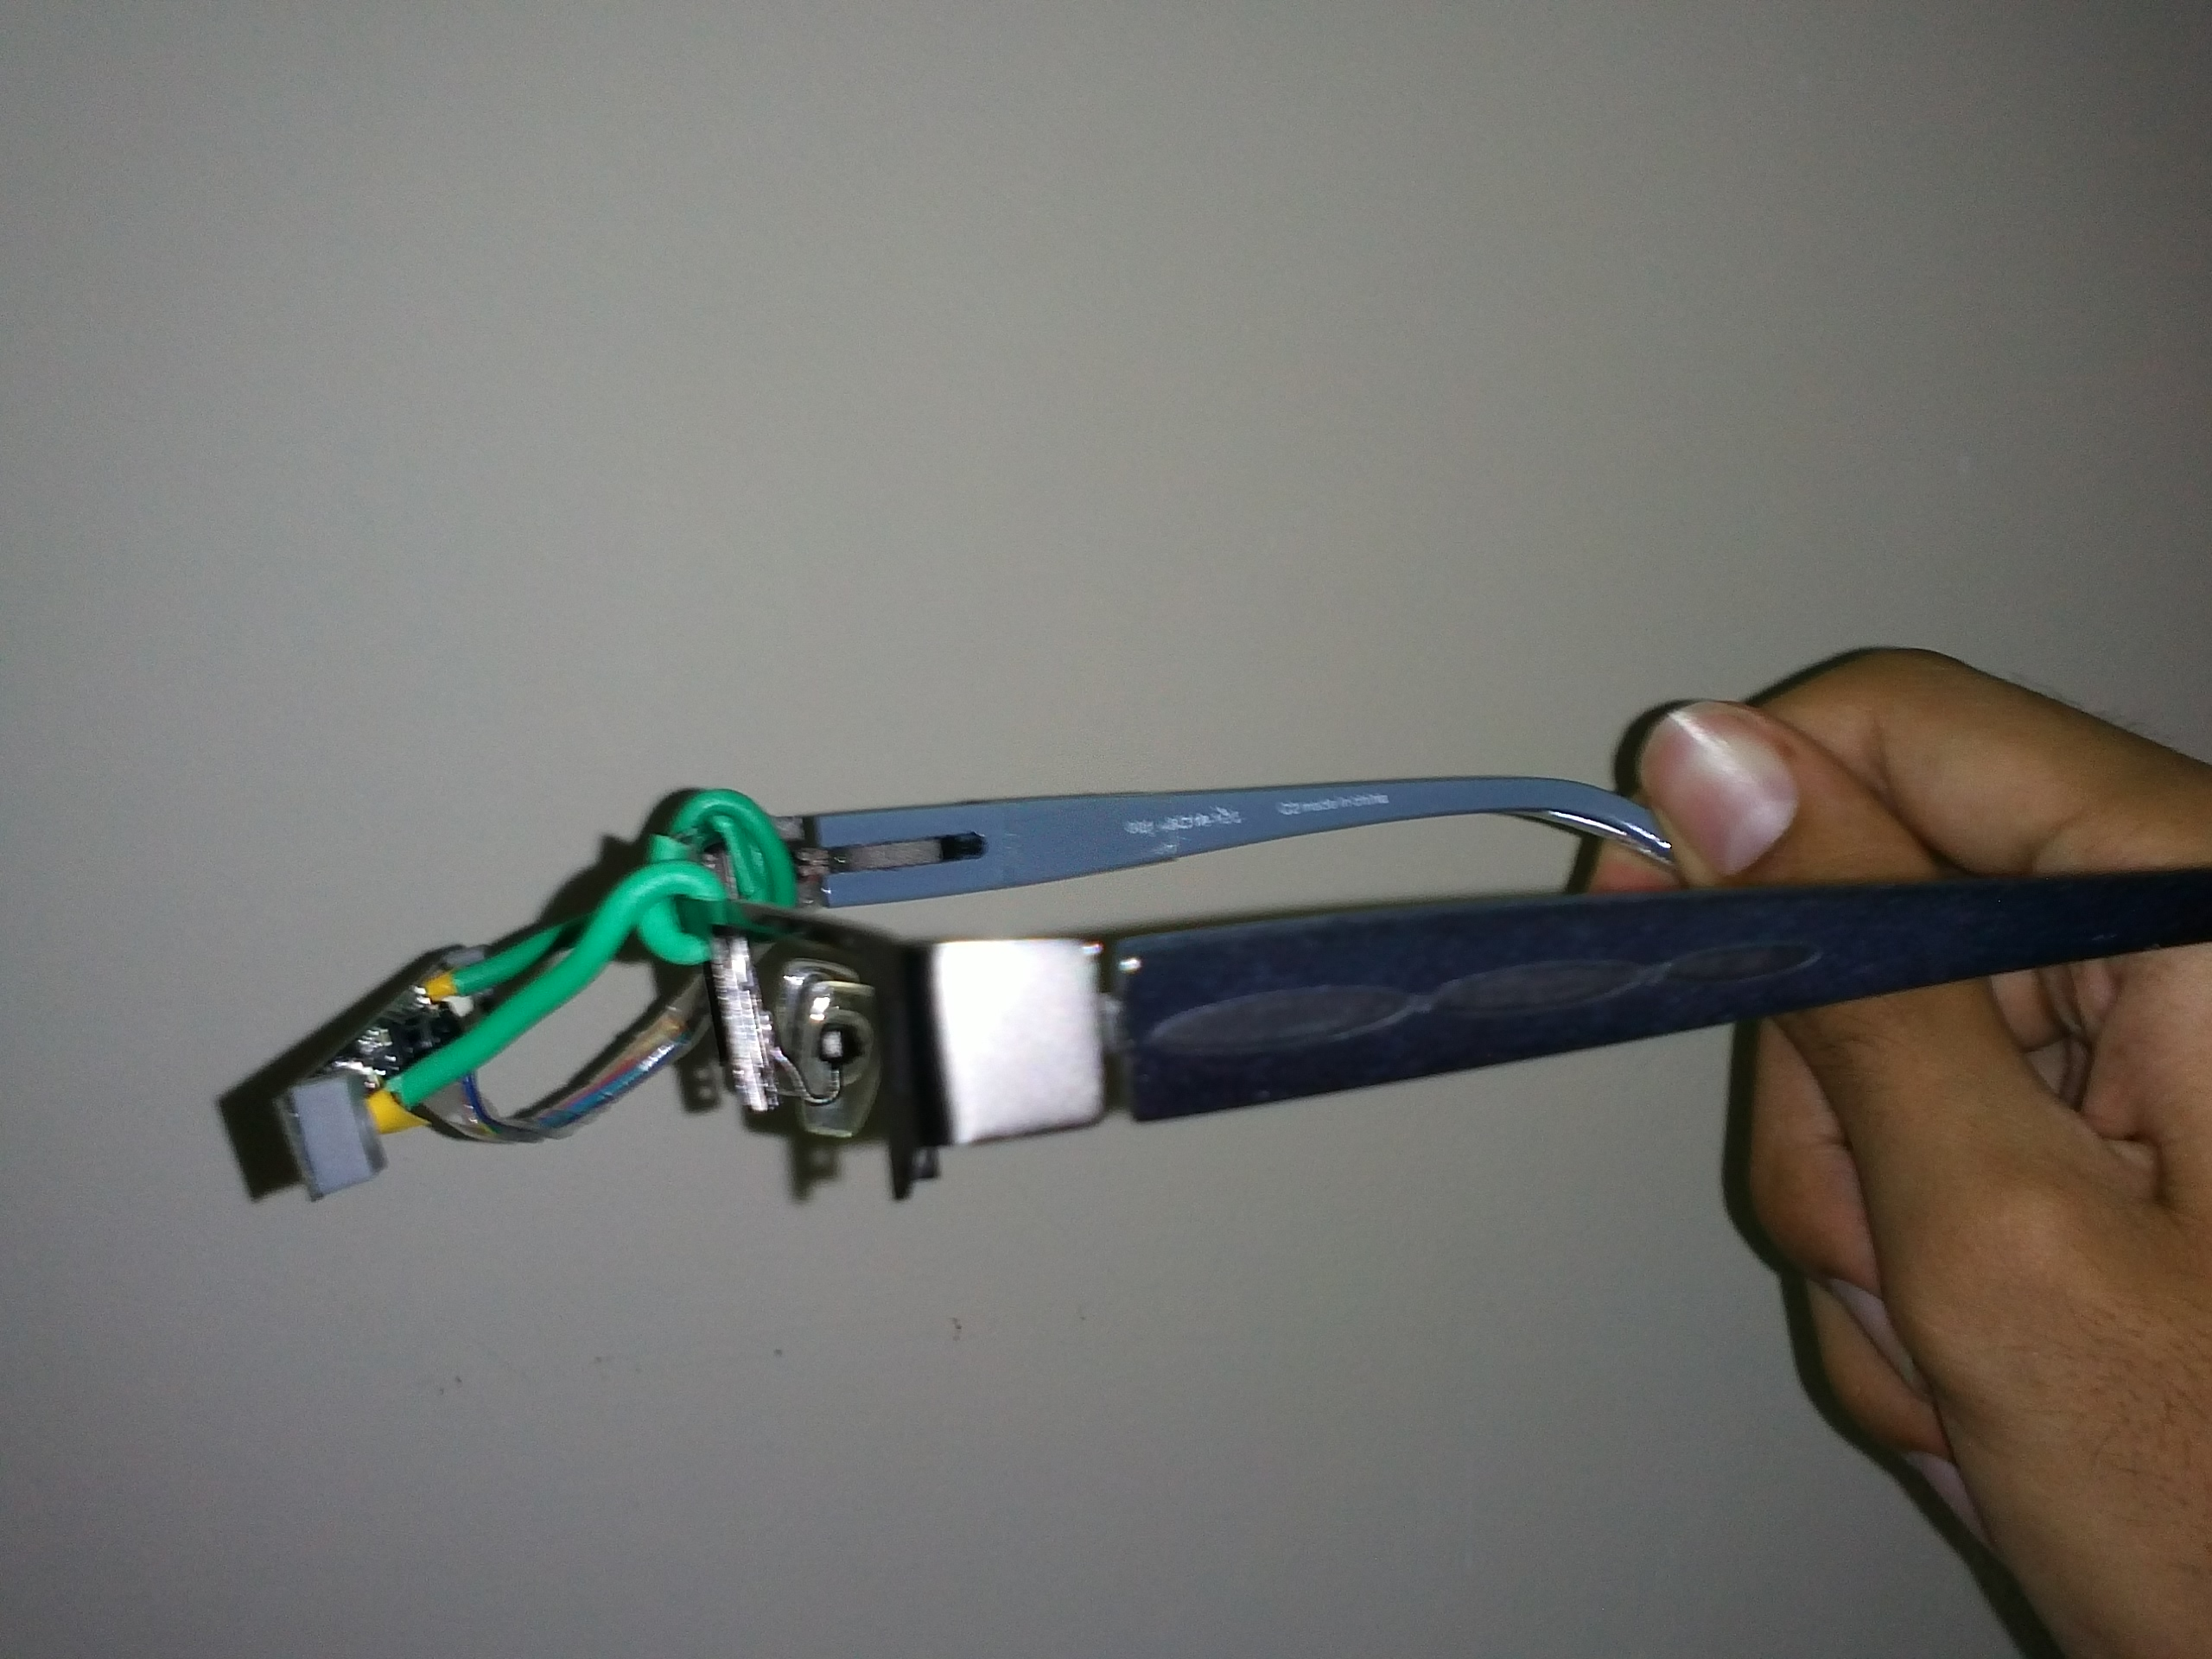
\includegraphics[width=.45\textwidth]{./Pictures/evaluation/cam_side_2.jpg}
	}
   \caption{Prototype of our cheap eye-tracking head set\label{fig:headset} }   
\end{dBox}   
\end{figure*}

%----------------------------------------------------------------------------------------
%	CHAPTER Gesture Recognition Introduction
%----------------------------------------------------------------------------------------
\chapterimage{cover_g_1.png} % Chapter heading image
\chapter{Gesture Recognition}
\section{Introduction and Related Work}\index{Introduction and Related Work}
Introduction part--Not added yet.
\bigskip

Methods for vision based hand gesture recognition fall into two categories: 3D model based methods and appearance model based methods. 3D model may exactly describe hand movement and its shape, but most of them are computational expensive to use. Recently there are some methods to obtain 3D model with 2D appearance model such as ISOSOM and PCA-ICA in \cite{relatedsg1} and \cite{relatedsg2}.
\bigskip

There have been a number of research efforts on appearance based method in recent years. Freeman and Weissman recognized gestures for television control using normalized correlation \cite{relatedsg3}. This technique is efficient but may be sensitive to different users, deformations of the pose and changes in scale, and background. Lars and Lindberg used scale-space color features to recognize hand gestures \cite{relatedsg4}. In their method, gesture recognition method is based on feature detection and user independent while the authors showed real-time application only under uniform backgrounds.
\bigskip

Yikai Fang, Kongqiao Wang proposed "A REAL-TIME HAND GESTURE RECOGNITION METHOD" \cite{relatedsg5} which based their work on Lars's work. They combine fast hand tracking, hand segmentation and multi-scale feature extraction to develop an accurate and robust hand gesture recognition method. It takes advantage of color and motion cues acquired during tracking to implement adaptive hand segmentation.
\bigskip

Our initial work was inspired by Yikai, Wang's work. We made an initial approach for hand detection and static gesture recognition based on the following procedure:\bigskip


\begin{itemize}
\item Detect hand from image based on:
\begin{itemize}
\item Skin color detection.
\item Hand is assumed to be the largest contour.
\end{itemize}
\item Extract Number of fingers, center of hand.
\item Identify gesture based on outputs from previous module using blocks of condition statements based on:
\begin{itemize}
\item Number of fingers.
\item Their angles with respect to x, y axis.
\end{itemize}
\end{itemize}
\bigskip

This approach has many problems that rise during the implementation:\bigskip


\begin{itemize}
\item There is a threshold to determine which points on the contour represent a finger point. That threshold is not reliable and sensitive to:
\begin{itemize}
\item Orientation of the hand.
\item Size of the hand.
\end{itemize}
\item Then we modified the threshold to be relative to hand size by using an equation that holds the hand width, height, and center point as variables.
That modification solves the reliability to hand size problem, but doesn't solve the orientation problem.
\item Unreliable if for example we want to distinguish between up gesture made by index finger, or thumb finger.
\end{itemize}
\bigskip

To solve the problems with the initial work, we directed our thoughts to machine learning. Where, we extract features from hand and use classification as described in paper \cite{relatedsg6}.
\bigskip

So we defined Three Approaches for static gestures. They differ on features used to represent the gesture:
\begin{enumerate}
\item Binary Representation Gridding as described in [link to that paper].
\item Predefined Feature Extraction as described in \cite{paper2sT}.
\item SIFT And Bag of Features Approach as described in [link to the paper].
\end{enumerate}
\bigskip


\section{Static Gestures}\index{Static Gestures}
This chapter includes the work done to detect static gestures. It begins by describing the general idea of segmentation and recognition and then proceeds to the following sections.\bigskip


\subsection{Prior Elaboration}\index{Prior Elaboration}
Segmentation is a very critical process. It depends majorly, in our case, on the detection of the hand, only the hand. That is why the lightest amount of noise could affect and diverge the result greatly. This is the reason behind noise elimination. It is an essential step prior to any segmentation process. We need to elaborate the image cleanly for the detector to easily find the item of interest among any other item in the image. Smoothing is considered the most effective solution in case of noise elimination. Many approaches have been devised to perform smoothing capably on the images just to keep the meaningful item for us unharmed in case there is any interference of any noise. The mask, filter, we use for noise elimination is Gaussian Smoothing.
need.\bigskip
\subsubsection{Gaussian Smoothing}\index{Prior Elaboraion}
The Gaussian smoothing operator is a 2-D convolution operator that is used to `blur' images and remove detail and noise. In this sense, it is similar to the mean filter, but it uses a different kernel that represents the shape of a Gaussian (`bell-shaped') hump. This kernel has some special properties which are detailed below.
\begin{figure*}[]
\begin{dBox}
\centering
  \mbox{
      \subfigure[Gaussian Distribution]{
            \label{fig:gaussian_1}
            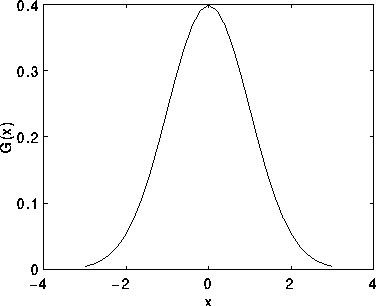
\includegraphics[width=.31\textwidth]{./Pictures/gesture/gaussian_distr.jpg}
        }
        \subfigure[Gaussian Distribution in 2D]{
           \label{fig:gaussian_2}
           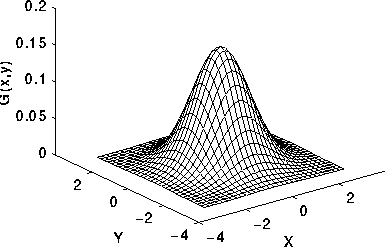
\includegraphics[width=.31\textwidth]{./Pictures/gesture/gaussian_distr_2d.png}
        }
   }
   \caption{Gaussian Distributions \label{fig:gaussian_dist} }   
\end{dBox}   
\end{figure*}
\bigskip
The Gaussian distribution in 1-D has the form:
\begin{dBox}
\begin{equation}
	G(x) = \frac{1}{\sqrt{2\pi\sigma}}e^{-\frac{x^2}{2\sigma^2}}
\end{equation}
\end{dBox}
where $\sigma$  is the standard deviation of the distribution. We have also assumed that the distribution has a mean of zero (i.e. it is centered on the line x=0). The distribution is illustrated in Figure \ref{fig:gaussian_dist}.
\bigskip
In 2-D, an isotropic (i.e. circularly symmetric) Gaussian has the form:
\begin{dBox}
\begin{equation}
	G(x,y) = \frac{1}{\sqrt{2\pi\sigma^2}}e^{-\frac{x^2+y^2}{2\sigma^2}}
\end{equation}
\end{dBox}
This distribution is shown in Figure \ref{fig:gaussian_dist}
\bigskip
The idea of Gaussian smoothing is to use this 2-D distribution as a `point-spread' function, and this is achieved by convolution. Since the image is stored as a collection of discrete pixels, we need to produce a discrete approximation to the Gaussian function before we can perform the convolution. In theory, the Gaussian distribution is non-zero everywhere, which would require an infinitely large convolution kernel, but in practice, it is effectively zero more than about three standard deviations from the mean, and so we can truncate the kernel at this point. Figure 3 shows a suitable integer-valued convolution kernel that approximates a Gaussian with a $\sigma$ of 1.0. It is not obvious how to pick the values of the mask to approximate a Gaussian.
%NOT FINISHED....................................
One could use the value of the Gaussian at the center of a pixel in the mask, but this 
is not accurate because the value of the Gaussian varies non-linearly across the pixel. We 
integrated the value of the Gaussian over the whole pixel (by summing the Gaussian at 0.001 
increments). The integrals are not integers: we rescaled the array so that the corners had the value 
1. Finally, the 273 is the sum of all the values in the mask. \bigskip

Once a suitable kernel has been calculated, then the Gaussian 
smoothing can be performed using standard convolution methods. 
The convolution can, in fact, be performed quickly since the 
equation for the 2-D isotropic Gaussian shown above is separable 
into x and y components. Thus, the 2-D convolution can be 
performed by first convolving with a 1-D Gaussian in 
the X direction, and then convolving with another 1-D Gaussian in 
the Y direction. (The Gaussian is in fact the only completely 
circularly symmetric operator that can be decomposed in such a 
way). 
%%%%%%%%%%%%%%%%%%%%%%%%%%%%%%%%%%%%%%%%%%%%%%%%%%%%%%
Figure \ref{fig:fig4} shows the 1-D x component kernel that would be used to produce the full kernel 
shown in Figure \ref{fig:fig3} (after scaling by 273, rounding and truncating one row of pixels around the 
boundary because they mostly have the value 0. This reduces the 7x7 matrix to the 5x5 shown 
above.). The Y component is exactly the same but is oriented vertically.

\begin{figure*}[h]
\begin{dBox}
\centering
  \mbox{
	    \subfigure[The full kernel]{
	          \includegraphics[width=.30\textwidth]{./Pictures/gesture/gaussian_kernal.png}
        }
   }
   \label{fig:fig3}   
\end{dBox}   
\end{figure*}

\begin{figure*}[h]
\begin{dBox}
\centering
  \mbox{
	    \subfigure[1-D x component kernel]{
	          \includegraphics[width=.60\textwidth]{./Pictures/gesture/row_table.jpg}
        }
   }
   \caption{ \label{fig:fig4} }   
\end{dBox}   
\end{figure*}


\bigskip
A further way to compute a Gaussian smoothing with a large 
standard deviation is to convolve an image several times with a 
smaller Gaussian. While this is computationally complex, it can have applicability if the processing 
is carried out using a hardware pipeline. 
\bigskip
The Gaussian filter not only has utility in engineering applications. It is also attracting attention 
from computational biologists because it has been attributed with some amount of biological 
plausibility, e.g. some cells in the visual pathways of the brain often have an approximately 
Gaussian response.

\bigskip
The effect of Gaussian smoothing is to blur an image, in a similar fashion to the mean filter. The 
degree of smoothing is determined by the standard deviation of the Gaussian. (Larger standard 
deviation Gaussians, of course, require larger convolution kernels in order to be accurately 
represented.) 

\bigskip
The Gaussian outputs a `weighted average' of each pixel's neighborhood, with the average 
weighted more towards the value of the central pixels. This is in contrast to the mean filter's 
uniformly weighted average. Because of this, a Gaussian provides gentler smoothing and 
preserves edges better than a similarly sized mean filter. 
\bigskip

One of the principle justifications for using 
the Gaussian as a smoothing filter is due 
to its frequency response. Most 
convolution-based smoothing filters act as 
lowpass frequency filters. This means that 
their effect is to remove high spatial 
frequency components from an image. The 
frequency response of a convolution 
filter, i.e. its effect on different spatial 
frequencies, can be seen by taking the 
Fourier transform of the filter. Figure \ref{fig:fig5}
shows the frequency responses of a 1-D mean filter with width 5 and also of a Gaussian filter 
with $\sigma$ = 3. We used figure \ref{fig:fig6} to illustrate the Gaussian's smoothing effect.

\begin{figure*}[h]
\begin{dBox}
\centering
  \mbox{
	    \subfigure[Frequency responses]{
	          \includegraphics[width=.80\textwidth]{./Pictures/gesture/freq_responses.jpg}
        }
   }
   \caption{Frequency responses \label{fig:fig5} }   
\end{dBox}   
\end{figure*}

\begin{figure*}[h]
\begin{dBox}
\centering
  \mbox{
      \subfigure[]{
            \label{fig:smooth1}
            \includegraphics[width=.31\textwidth]{./Pictures/gesture/smooth1.jpg}
        }
        \subfigure[]{
           \label{fig:smooth2}
           \includegraphics[width=.31\textwidth]{./Pictures/gesture/smooth2.jpg}
        }
        \subfigure[]{
            \label{fig:sift_3}
            \includegraphics[width=.31\textwidth]{./Pictures/gesture/smooth3.jpg}
       }
   }
   \caption{Gaussian's smoothing effect \label{fig:fig6} }   
\end{dBox}   
\end{figure*}


We used an appropriate value for $\sigma$ and a kernel size 5*5 in our work. Of course, the higher 
kernel size we provide, the better smoothing we get, but the problem resides in the processing 
overhead. Since we have more processing coming head in several parts coming ahead we cannot 
just strain it and delay it here. Therefore, a secured limit of smoothing is sufficient to avoid the 
results that could harm the further work coming ahead. 
\bigskip


\subsubsection{Color Segmentation }\index{Color Segmentation }
Color image segmentation is useful in many applications. From the segmentation results, it is 
possible to identify regions of interest and objects in the scene, which is very beneficial to the 
subsequent image analysis or annotation. The problem of segmentation is difficult because of 
image texture. If an image contains only homogeneous color regions, clustering methods in color 
space are sufficient to handle the problem. In reality, natural scenes are rich in color and texture. 
It is difficult to identify image regions containing color-texture patterns.\bigskip

Color images are usually represented in terms of their Red, Green and Blue components (RGB 
format) for purposes of storage and display. All of the color spaces can be derived from the RGB 
information supplied by devices such as cameras and scanners. The RGB color space is the most 
prevalent choice for computer graphics because color displays use red, green, and blue to create 
the desired color. Therefore, the choice of the RGB color space simplifies the architecture and 
design of the system. Furthermore, a system that is designed using the RGB color space can 
take advantage of a large number of existing software routines, since this color space has been 
around for a number of years.  \bigskip

However, RGB is not very efficient when dealing with "real-world" images. All three RGB 
components need to be of equal bandwidth to generate any color within the RGB color cube. 
The result of this is a frame buffer that has the same pixel depth and display resolution for each RGB component. In addition, processing an image in the RGB color space is usually not the 
most efficient method. For example, to modify the intensity or color of a given pixel, the three 
RGB values must be read from the frame buffer, the intensity or color calculated, the desired 
modifications performed, and the new RGB values calculated and written back to the frame 
buffer. If the system had access to an image stored directly in the intensity and color format, 
some processing steps would be faster. That is why we need desperately to move from RGB to 
another domain, where segmentation is more reliable. We have found it most beneficial to 
convert to YCBCr color space. \bigskip

The YCbCr color space is widely used for digital video. In this format, luminance information is 
stored as a single component (Y), and chrominance information is stored as two color-difference 
components (Cb and Cr). Cb represents the difference between the blue component and a 
reference value. Cr represents the difference between the red component and a reference value. \bigskip


YCbCr data can be double precision, but the color space is particularly well suited 
to uint8 data. For uint8 images, the data range for Y is [16, 235], and the range for Cb and Cr is 
[16, 240]. YCbCr leaves room at the top and bottom of the full uint8 range so that additional 
(nonimage) information can be included in a video stream. From YCbCr we apply a threshold 
on this color space to convert the image to the grayscale image.\bigskip

The resulting conversion, based on a threshold, may result in a noise that we don't desire them 
to exist. This noise is totally hazard to the further processing of the image. Which means that 
we need another smoothing step. This time the smoothing requires us to preserve certain details 
in the image, which are the edges of our items of interest. Consequently, we need a conservative 
smoothing that could secure us to preserve edges, which introduces us to the median filter.\bigskip

\subsubsection{Conservative Smoothing (Median Filter)} \index{Conservative Smoothing (Median Filter)}
Conservative smoothing is a noise reduction technique that derives its name from the fact that it 
employs a simple, fast filtering algorithm that sacrifices noise suppression power in order to 
preserve the high spatial frequency detail (e.g. sharp edges) in an image. It is explicitly designed 
to remove noise spikes --- i.e. isolated pixels of exceptionally low or high pixel intensity (e.g. salt 
and pepper noise) and is, therefore, less effective at removing additive noise (e.g. Gaussian noise) 
from an image.  \bigskip

Like most noise filters, conservative smoothing operates on the assumption that noise has a 
high spatial frequency and, therefore, can be attenuated by a local operation which makes each 
pixel's intensity roughly consistent with those of its nearest neighbors. However, whereas mean 
filtering accomplishes this by averaging local intensities and median filtering by a non-linear 
rank selection technique, conservative smoothing simply ensures that each pixel's intensity is 
bounded within the range of intensities defined by its neighbors.  \bigskip

The median filter is normally used to 
reduce noise in an image, somewhat 
like the mean filter. However, it often 
does a better job than the mean filter 
of preserving useful detail in the 
image. Like the mean filter, the 
median filter considers each pixel in 
the image in turn and looks at its 
nearby neighbors to decide whether or 
not it is representative of its 
surroundings. Instead of simply replacing the pixel value with the mean of neighboring pixel 
values, it replaces it with the median of those values. The median is calculated by first sorting 
all the pixel values from the surrounding neighborhood into numerical order and then replacing 
the pixel being considered with the middle pixel value. (If the neighborhood under consideration 
contains an even number of pixels, the average of the two middle pixel values is used.) Figure \ref{fig:fig7}
illustrates an example calculation.

\begin{figure*}[h]
\begin{dBox}
\centering
\mbox{
	    \subfigure[]{
	          \includegraphics[width=.80\textwidth]{./Pictures/gesture/median.jpg}
        }
   }
   \caption{
   \label{fig:fig7} }   
\end{dBox}   
\end{figure*}
\bigskip

By calculating the median value of a neighborhood rather than the mean filter, the median filter 
has two main advantages over the mean filter: 
\begin{itemize}
\item The median is a more robust average than the mean and so a single very 
unrepresentative pixel in a neighborhood will not affect the median value significantly. 
\item Since the median value must actually be the value of one of the pixels in the 
neighborhood, the median filter does not create new unrealistic pixel values when the 
filter straddles an edge. For this reason, the median filter is much better at preserving 
sharp edges than the mean filter.
\end{itemize}

Figure \ref{fig:fig8} illustrates the effect of the median filter with many kernel sizes. At our 
work, we used the median filter with kernel size 5*5. It was most convenient for our work and 
this size preserved the edges the way we would like it to be. 
\begin{figure*}[h]
\begin{dBox}
\centering
  \mbox{
      \subfigure[]{
            \label{fig:median_1}
            \includegraphics[width=.31\textwidth]{./Pictures/gesture/smooth_median_1.jpg}
        }
        \subfigure[]{
           \label{fig:median_2}
           \includegraphics[width=.31\textwidth]{./Pictures/gesture/smooth_median_2.jpg}
        }
        \subfigure[]{
            \label{fig:median_3}
            \includegraphics[width=.31\textwidth]{./Pictures/gesture/smooth_median_3.jpg}
       }
   }
   \caption{Median Filter \label{fig:fig8} }   
\end{dBox}   
\end{figure*}

\subsubsection{Binary Image and Connected Components}\index{Binary Image and Connected Components}
NOT YET

\subsection{Algorithm one: Binary Representation}\index{Algorithm one: Binary Representation}

The algorithm as described in \cite{paper1sb} takes the hand in the binary from as shown in Figure \ref{fig:grid_idea} (a).
The general idea of the algorithm is that we need parts of the image to vote for their existence but not pixel by pixel to decrease processing time. So the algorithm divides the binary image into grids as shown in Figure \ref{fig:grid_idea} (b).
\begin{figure*}[h]
\begin{dBox}
\centering
  \mbox{
   \subfigure[Open Hand]{
            \label{fig:binary_ofp}
            \includegraphics[width=.31\textwidth]{./Pictures/gesture/binary_open.jpg}
        }
      \subfigure[Grid Idea]{
            \label{fig:binary_op}
            \includegraphics[width=.30\textwidth]{./Pictures/gesture/gridding_idea.jpg}
        }
       
        }
   \caption{Binary Image and its gridding  \label{fig:grid_idea} }   
\end{dBox}   
\end{figure*}
And let each grid's vote represent the votes of its pixels. Each grid votes according to its state as shown in Figure \ref{fig:vote_idea}.\bigskip
 \begin{figure*}[h]
\begin{dBox}
\centering
  \mbox{
      \subfigure[]{
            \label{fig:vote_cases}
            \includegraphics[width=.8\textwidth]{./Pictures/gesture/vote_cases.png}
        }
       
        }
  \caption{ Grids Vote Cases \label{fig:vote_idea} }   
\end{dBox}   
\end{figure*}

The Whole case and the voting determination process is explained bye the flow chart in Figure \ref{fig:vfc}

\begin{figure*}[]
\begin{dBox}
\centering
  \mbox{
      \subfigure[]{
            \label{fig:binary_op_alg}
            \includegraphics[width=.8\textwidth]{./Pictures/gesture/vfc.png}
        }
       
        }
   \caption{Voting Flow Chart \label{fig:vfc} }   
\end{dBox}   
\end{figure*}
\bigskip

% The algorithm as described in \cite{paper1sb} is based on describing the image, compare this description, and classify it with the help of the data set after walking through the previously mentioned steps for elaborating the image and extracting the hand in binary representation, an example for a binary image is shown in figure \ref{fig:open_binary}. Standardly, we now have an image that contains two meaningful details only the foreground pixels that should only represent the hand and the background pixels that only represent the background. Generally, to describe an image we need every pixel of image to declare itself, vote whether it is foreground or background, and then we can have the general visualization for the image by traversing ever pixel and checking what it looks like. Therefore, to traverse ever pixel this is a huge processing consumption given that we have many frames coming in it is needless to do a per pixel checking for each image in each frame. \bigskip
% \begin{figure*}[h]
% \begin{dBox}
% \centering
%   \mbox{
%       \subfigure[Open Hand]{
%             \label{fig:binary_op}
%             \includegraphics[width=.31\textwidth]{./Pictures/gesture/binary_open.jpg}
%         }
       
%         }
%   \caption{Binary Image Example \label{fig:open_binary} }   
% \end{dBox}   
% \end{figure*}

% Our algorithm alleviates such processing burden. The general idea of the algorithm includes this voting but in a less processing way. We need parts of the image to vote on their existence but not pixel by pixel. Given the binary image, it is quite visible that most of the pixels are going to declare themselves a background pixel or, at the best fitting, we find the same number of pixels on foreground and background. However, this is still a waste of processing. The algorithm we are about to detail its idea starts by introducing what can resolve this needless processing waste, the griding. \bigskip

% \subsubsection{Griding The Binary Image}\index{Algorithm Two: Binary Representation}
% Our Work begins by dividing the binary image we obtained from our elaboration steps into grids as shown in Figure \ref{fig:grid_idea}. The griding is an alternative approach for pixel-by-pixel traversing. In this approximation, we just process n grids, standardly, rather than over thousands and thousands of pixels. This solution is based on the nature of the input image as a binary image. It may not work if the image is not binary image. The binary representation helps us limit any grid value to either 0 or 1 according to the voting technique we use.\bigskip
% \begin{figure*}[h]
% \begin{dBox}
% \centering
%   \mbox{
%       \subfigure[]{
%             \label{fig:binary_op}
%             \includegraphics[width=.31\textwidth]{./Pictures/gesture/gridding_idea.jpg}
%         }
       
%         }
%   \caption{Griding Idea Example \label{fig:grid_idea} }   
% \end{dBox}   
% \end{figure*}

% \subsubsection{Grid Voting}\index{Algorithm Two: Binary Representation}
% As the image is a binary image, some grids vote according to one of the following cases in Figure \ref{fig:vote_idea}
% \bigskip

% \begin{figure*}[h]
% \begin{dBox}
% \centering
%   \mbox{
%       \subfigure[]{
%             \label{fig:vote_cases}
%             \includegraphics[width=.8\textwidth]{./Pictures/gesture/vote_cases.png}
%         }
       
%         }
%   \caption{ Grids Vote Cases \label{fig:vote_idea} }   
% \end{dBox}   
% \end{figure*}
% \paragraph{$1^{st}$ Case: Totally Background}\index{Grid Voting}
% In this case, the whole grid is formed by background pixels only as shown in Figure \ref{fig:vote_cases_d} (a), all of them are black pixels. Consequently, the grid votes on its value to be 0. Note that to know this nature about a grid we traverse its pixels. This is not reverting us back to the pixel-by-pixel approach but, here, we just traverse until we encounter the existence of a one white pixel only. This white pixel is always interpreted as a foreground pixel and this moves us to the second case. Therefore, we are not traversing all the pixels this just happens in the grids that contain no foreground pixels but generally, the voting is determined after the traversing is done once we hit the end of the grid and no foreground pixels exist or once we come across a foreground pixel. Which guarantees the running time and the processing time to be kept lower than the former approach that counts the voting of ever pixel.
% \begin{figure*}[h]
% \begin{dBox}
% \centering
%   \mbox{
%       \subfigure[Case 1]{
%             \label{fig:black}
%             \includegraphics[width=.18\textwidth]{./Pictures/gesture/black_cell.jpg}
%         }
%         \subfigure[Case 2]{
%           \label{fig:partial}
%           \includegraphics[width=.63\textwidth]{./Pictures/gesture/partially.jpg}
%         }
%         \subfigure[Case 3]{
%           \label{fig:white}
%           \includegraphics[width=.18\textwidth]{./Pictures/gesture/white_cell.jpg}
%         }
%   }
%   \caption{Grid Shapes \label{fig:vote_cases_d} }   
% \end{dBox}   
% \end{figure*}

% \paragraph{$2^{nd}$ Case: Partially Background}\index{Grid Voting}
% Different from the first case, the image's grid, in this one, encounters the presence of two kinds of pixels; background and foreground. Check examples in Figure \ref{fig:vote_cases_d}.
% In this case, the voting is determined directly, without traversing, if the first pixel in the grid is a foreground pixel. However there could be a background pixels in the upcoming parts of the grid but we don't need to traverse for the rest of pixels, as the voting immediately turns to "1" once we find this white pixel. Otherwise, if the first pixel is background pixel, hence, we begin in the same way as the first case until we hit the presence of a foreground pixel then the traversing is terminated and the vote of the whole grid turns to "1". If no foreground pixels detected, then the voting remains "0" as in the first case. The grid that can be seen as an edge grid is the one that can be described via this case. The traversing stops at the yellow points which explains the variety of this case.
% All these sub-cases are shown in Figure \ref{fig:vote_cases_d} (b).\bigskip
% \paragraph{$3^{rd}$ Case: Totally Foreground}\index{Grid Voting}
% There is no much difference between this case and the previous one. In both cases, we encounter the presence of foreground pixels but this case can be considered a special case from the previous case since we have no background pixels. Which means that the grid is totally foreground. This can be interpreted that the grid is not an edge grid, as it has nothing from the background. As show in Figure \ref{fig:vote_cases_d}(c).

% The Whole case and the vote determination is explained by the flow chart in Figure \ref{fig:vfc}.
% \begin{figure*}[]
% \begin{dBox}
% \centering
%   \mbox{
%       \subfigure[]{
%             \label{fig:binary_op_alg}
%             \includegraphics[width=.6\textwidth]{./Pictures/gesture/vfc.png}
%         }
       
%         }
%   \caption{Voting Flow Chart \label{fig:vfc} }   
% \end{dBox}   
% \end{figure*}
% \bigskip


The griding approximation is acting as if we let group of pixels decides rather than pixel by pixel. On the one hand, this counts best for the processing performance, much better, but on the other hand, that doesn't sound promising for the accuracy. To illustrate this clearly let us consider and talk about the following example if we choose the griding to be only 2*2 grids. At this case, we may have the binary shape of the hand, in any form. While detection, it will always results in a just four grids and all of them are voted to be 1. Another case, if we used 5*5 grids. This results in a completely different voting result. Furthermore, if we used 10*10 grids, the resulting voting is presented in the Figure \ref{fig:bin_sizes} (a,b,c)
\begin{figure}[h]
\begin{dBox}
\centering
  \mbox{
      \subfigure[n=2]{
            \label{fig:n2}
            \includegraphics[width=.33\textwidth]{./Pictures/gesture/n2.jpg}
        }
        \subfigure[n=5]{
           \label{fig:n5}
           \includegraphics[width=.33\textwidth]{./Pictures/gesture/n5.jpg}
        }
        \subfigure[n=10]{
           \label{fig:n10}
           \includegraphics[width=.33\textwidth]{./Pictures/gesture/n10.jpg}
        }
   }
   \caption{Voting Results Using Different Grid Sizes \label{fig:bin_sizes} }   
\end{dBox}   
\end{figure}
\bigskip

The pixel-by-pixel detection gives us an optimal description and yet the worst performance but we can approximate our approach to go nearer to this optimal description and yet preserves the performance. This can be achieved if we choose a larger number of grids that can actually be considered as if they are pixels not girds. The larger we keep the number of girds growing to be, the better accuracy we obtain, and the worse the performance gets.\bigskip
% This keeps happening as long as we increase the number of girds until the grid is actually a pixel, then, the worst performance occur and the best accuracy is obtained.\bigskip

The following table shows the effect of The grid size on accuracy and running time:
\bigskip
\begin{center}
\begin{tabular}{ |c|c|c| }
 \hline
 Grid Size & Accuracy & Average Running Time \\
 \hline
 N = 5 & 81 \%  & 35 ms \\
 \hline
 N = 10 & 88 \%  & 60 ms\\
 \hline
 N = 15 & 91 \%  & 90 ms\\
 \hline
\end{tabular}
\end{center}
% The reason why this happens can be see clearly in table (Not Yet). When we increase the grid size, we happen to include more details in each grid that can be described optimally and totally by pixel-by-pixel approach. As long as we make the grids come across edges in a way that griding attempts to preserve the shape of the binary image, our accuracy will rapidly grow. Therefore, to conclude, more girds better accuracy. Every time we enlarge the gird size we check the accuracy and performance until we hit this number of grids that gives acceptable results on each as recorded in table (Not Yet).\bigskip

% The previous figures also assert what we were saying about the indispensability of noise elimination. Since, if we got one white noisy spot in the image it will significantly affect the resulting matrix and affect all that is following this step.
% \subsubsection{Flatting The Votes}\index{Algorithm Two: Binary Representation}
After each gird's voting is determined, now we get a matrix of 0s and 1s. This matrix represents the feature array which will be passed to the classifier either for training/evaluating.

We get to detail how the classifiers we used to evaluate and test our algorithm work in the classification chapter.


\subsection{Algorithm Two: Predefined Features Extraction}\index{Algorithm Two: Predefined Features Extraction}
Feature extraction is a crucial step in computer vision applications for hand gesture recognition. The pre-processing stage prepares the input image and extracts features used later with the classification algorithms. This set of features shall be unique per ever gesture. The set of features the algorithm generates based on \cite{paper2sT} are as follow:
\bigskip
\begin{itemize}
\item Mean and Variance of the gray pixel values.
\item The hand area and perimeter.
\item Hand orientation.
\item Orientation histogram.
\item Radial signature.
\end{itemize}
\bigskip
\begin{figure*}[h]
\begin{dBox}
\centering
  \mbox{
      \subfigure[Mean and variance]{
            \label{fig:mean_var}
            \includegraphics[width=.5\textwidth]{./Pictures/gesture/mean_var.jpg}
        }
        \subfigure[Area and perimter]{
           \label{fig:area}
           \includegraphics[width=.5\textwidth]{./Pictures/gesture/area.jpg}
        }
   }
   \caption{First Two Features \cite{paper2sT} \label{fig:mean_area} }   
\end{dBox}   
\end{figure*}
\bigskip
The first two features: mean, variance and the blob area and perimeter are detected from the previous steps prior to the algorithm. The smoothing followed by obtaining the gray image helps us finding the mean and the variance of the gray pixel values that represent the blob according to figure \ref{fig:mean_area}. The blob area and perimeter are detected from the last elaboration step which is finding the binary image for the blob. Figure \ref{fig:mean_area} illustrates how this works. The area of the white region is calculated approximated and then the perimeter is determined on the position of the hand on the image. This now leaves us with the rest of the five other features remaining to find in the set.
\bigskip
\subsubsection{Hand Orientation}\index{Algorithm One: Predefined Features Extraction}
The segmented hand is used to calculate its orientation with the help of image moments. Moment approximations provide one of the more obvious means of describing 2-D shapes\cite{feature1}. The moments involve sums over all pixels, and so are robust against small pixel changes\cite{feature2}. If I x, y is the image intensity at position x and y then the image moments, up to the second order, are:
\bigskip
\begin{dBox}
\begin{equation}
	M_{00}= \sum_{x}\sum_{y}I(x,y)
\end{equation}
\begin{equation}
	M_{01}= \sum_{x}\sum_{y}y.I(x,y)
\end{equation}
\begin{equation}
	M_{10}= \sum_{x}\sum_{y}x.I(x,y)
\end{equation}
\begin{equation}
	M_{11}= \sum_{x}\sum_{y}xy.I(x,y)
\end{equation}
\begin{equation}
	M_{20}= \sum_{x}\sum_{y}x^{2}I(x,y)
\end{equation}
\begin{equation}
	M_{02}= \sum_{x}\sum_{y}y^{2}I(x,y)
\end{equation}
\end{dBox}
\bigskip
The hand position can be calculated as follows:
\bigskip
\begin{dBox}
\begin{equation}
	x_{c} = \frac{M_{10}}{M_{00}}
\end{equation}
\begin{equation}
	y_{c} = \frac{M_{01}}{M_{00}}
\end{equation}
\end{dBox}
\bigskip
The hand orientation can then be calculated using the following intermediate variables a, b and c:
\bigskip
\begin{dBox}
\begin{equation}
	a = \frac{M_{20}}{M_{00}} - x_{c}^{2}
\end{equation}
\begin{equation}
	b = 2 (\frac{M_{10}}{M_{00}}-x_{c}y_{c})
\end{equation}
\begin{equation}
    c = \frac{M_{02}}{M_{00}}- y_{c}^{2}
\end{equation}
\end{dBox}
\bigskip
and the angle is:
\begin{dBox}
\begin{equation}
\theta = \frac{tan^{-1}(b,(a-c))}{2}
\end{equation}
\end{dBox}
\bigskip
\subsubsection{Orientation Histogram}\index{Algorithm One: Predefined Features Extraction}
Pixel intensities can be sensitive to lighting variations,
which lead to classification problems within the same gesture under different light conditions. The use of local
orientation measures avoids this kind of problem, and the
histogram gives us translation invariance. Orientation
histograms summarize how much of each shape is oriented in each possible direction, independent of the position of the hand inside the camera frame\cite{feature2}.\bigskip

This statistical technique is most appropriate for close-ups of the hand. In our work, the hand is extracted and separated from the background. This provides a uniform black background, which makes this statistical technique a good method for the identification of different static hand poses. This method is insensitive to small changes in the size of the hand, but it is sensitive to changes in hand orientation.\bigskip

We have calculated the local orientation using image gradients, represented by horizontal and vertical image pixel differences. If dx and dy are the outputs of the derivative operators, then the gradient direction is $arctan(dx,dy)$ and the contrast is  $\sqrt{d_{x}^{2}+d_{y}^{2}}$ A contrast threshold is set as some amount k times the mean image contrast, below which we assume the orientation measurement is inaccurate. A value of k=1.2 was used in the experiments. We then blur the histogram in the angular domain as in\cite{feature3} with a [1 4 6 4 1] filter, which gives a gradual fall-off in the distance between orientation histograms.\bigskip

Our histogram of orientation is composed of 36 bins, which means that this feature is described via 36 values.
\bigskip
\subsubsection{Radial Signature}\index{Algorithm One: Predefined Features Extraction}
A simple method to assess the gesture would be to measure the distance from the hand centroid to the edges of the hand along a number of equally spaced radials \cite{feature4} around a circle. This would provide information on the general "shape" of the gesture that could be easily rotated to account for hand yaw (since any radial could be used as datum).
\bigskip
Figure \ref{fig:radial_sig} (a) shows a gesture with example radials (simplified).
However, a problem (as shown in Figure \ref{fig:radial_sig} (a) ) is how to measure when the radial crosses a gap between fingers or between the palm and a finger. To remedy this it was decided to count the total number of skin pixels along a given radial. This is shown in Figure \ref{fig:radial_sig} (b). All of the radial measurements could then be scaled so that the longest radial was of constant length. By doing this, any alteration in the hand camera distance would not affect the radial length signature generated.

\begin{figure*}[h]
\begin{dBox}
\centering
  \mbox{
      \subfigure[Radial Idea]{
            \label{fig:radial}
            \includegraphics[width=.31\textwidth]{./Pictures/gesture/radial.jpg}
        }
        \subfigure[Corrected Radial]{
           \label{fig:radial_2}
           \includegraphics[width=.31\textwidth]{./Pictures/gesture/radial2.jpg}
        }
   }
   \caption{Radial Signature \cite{feature4} \label{fig:radial_sig} }   
\end{dBox}   
\end{figure*}

A simple method to assess the gesture would be to measure the distance from the hand centroid to the edges of the hand along a number of equally spaced radials. For the present feature extraction problem, 100 equally spaced radials were used. To count the number of pixels along a given radial we only take into account the ones that are part of the hand, eliminating those that fall inside gaps, like the ones that appear between fingers or between the palm and a finger.
\bigskip

During tests it was noticed that the quality of recognition depended on the number of radials used. It was also noticed that most of the significant data was concentrated around the fingers, thus it would be more efficient to group radials in these areas. Figure \ref{fig:radial_bins} shows the radials in their original grouping and after reorganization.
\bigskip
\begin{figure*}[h]
\begin{dBox}
\centering
  \mbox{
      \subfigure[Radial Signature with bin=100]{
            \label{fig:ori_bin}
            \includegraphics[width=.31\textwidth]{./Pictures/gesture/ori_bins.jpg}
        }
        \subfigure[Radial Signature with bin=100]{
           \label{fig:inc_bin}
           \includegraphics[width=.31\textwidth]{./Pictures/gesture/inc_bins.jpg}
        }
   }
   \caption{Radial Signature with different bin sizes\cite{feature4} \label{fig:radial_bins} }   
\end{dBox}   
\end{figure*}

All the radial measurements can be scaled so that the longest radial has a constant length. With this measure, we can have a radial length signature that is invariant to hand distance from the camera.

\subsection{Gesture Recognition Using Bag-of-Features and Classification.}\index{Gesture Recognition Using Bag-of-Features and Classification}
\subsubsection*{Introduction}
Content based image retrieval (CBIR) is still an active research field. There are a number of approaches available to retrieve visual data from large databases. But almost all the approaches require an image digestion in their initial steps. Image digestion is describing an image using low level features such as color, shape, and texture while removing unimportant details. Color histograms, color moments, dominant color, scalable color, shape contour, shape region, homogeneous texture, texture browsing, and edge histogram are some of the popular descriptors that are used in CBIR applications. Bag-Of-Feature (BoF) is another kind of visual feature descriptor which can be used in CBIR applications. In order to obtain a BoF descriptor we need to extract a feature from the image. This feature can be any thing such as SIFT (Scale Invariant Feature Transform), SURF (Speeded Up Robust Features), and LBP (Local Binary Patterns), etc.\bigskip

In this system we are using the Scale Invariant Feature Transform (SIFT) features \cite{sift}. These visual features/keypoints allow for reliable matching between different views of the same object, image classification, and object recognition. The SIFT features/keypoints are invariant to scale, orientation, and partially invariant to illumination changes, and are highly distinctive of the image. However, SIFT features are too high dimensionality to be used efficiently. We propose to solve this problem by using the bag-of-features approach \cite{Lazebn06} to reduce the
dimensionality of the feature space. \bigskip


\subsubsection{Features Extraction Using SIFT} \index{Features Extraction Using SIFT}
Features based on the SIFT algorithm are invariant to scale and rotation and can be 
extracted in real-time for low resolution images. They are extracted in four stages. The first step 
finds the locations of potential interest points in the image by detecting the maxima and minima 
of a set of difference of Gaussian filters applied at different scales all over the image. Then, these 
locations are refined by eliminating points of low contrast. An orientation is then assigned to 
each keypoint based on local image features. Finally, a local feature descriptor is computed at 
each keypoint. This descriptor is based on the local image gradient transformed according to the 
orientation of the keypoint for providing orientation invariance. The size of the feature vector 
depends on the number of histograms and the number of bins in each histogram. In Lowe's 
original implementation\cite{sift} a 4-by-4 patch of histograms with 8 bins each is used, 
generating a 128-dimensional feature vector. See Figure \ref{fig:sift_example} for example of extracted features. Each features is descripted using 1D array of numbers. 

\begin{figure*}[]
\begin{dBox}
\centering
  \mbox{
      \subfigure[Open Hand]{
            \label{fig:sift_1}
            \includegraphics[width=.31\textwidth]{./Pictures/gesture/call_0_SIFT.jpg}
        }
        \subfigure[Closed Hand]{
           \label{fig:sift_2}
           \includegraphics[width=.31\textwidth]{./Pictures/gesture/closed_10_SIFT.jpg}
        }
        \subfigure[Hand pointing to left]{
            \label{fig:sift_3}
            \includegraphics[width=.31\textwidth]{./Pictures/gesture/left_0_SIFT.jpg}
       }
   }
   \caption{SIFT features \label{fig:sift_example} }   
\end{dBox}   
\end{figure*}
\bigskip

\subsubsection{K-Means Clustering} \index{K-Means Clustering}
Clustering divides a group into subgroups, called clusters, so that the elements in the 
same cluster are similar. It is implemented using an unsupervised learning algorithm and an 
ordinary method for statistical data analysis applied in several fields, such as machine learning, 
pattern recognition, image analysis, data mining, and bioinformatics.
\bigskip

The number of clusters (the codebook size) depends on the structure of 
the data. There will be a compromise for how to choose the vocabulary size or number of 
clusters. If it is too small, then each bag-of-words vector will not represent all of the keypoints 
extracted from its related image. If it is too large, it will lead to overfitting because of insufficient 
samples of the keypoints extracted from the training image. 
We trained the classifier using 234 images with number of bags equal to 200. This number provides the most accurate recognition rate by trying different values \cite{Dardas11}.

\bigskip
The first step in k-means clustering is to divide the vector space (128-dimensional feature 
vector) into k clusters. K-means clustering starts with k randomly located centroids (points in space that represent the center of the cluster) and assigns every keypoint to the nearest one. After 
the assignment, the centroids (codevectors) are shifted to the average location of all the 
keypoints assigned to them, and assignments are redone. This procedure repeats until the 
assignments stop changing.

\bigskip
Once this is done, each feature vector (keypoint) is assigned to one and only one cluster 
center that is in the nearest distance with respect to the Euclidean distance metric in the 128-
dimensional feature vectors. The keypoints that are assigned to the same cluster center will be in 
the same subgroup so that after clustering, we have k disjoint subgroups of keypoints. Therefore, 
k-means clustering decreases the dimensionality for every training image with n keypoints 
(nx128) to 1xk, where k is the number of clusters.


\subsubsection{Classification} \index{Classification}
All the keypoints recovered in the training images are mapped with its generated bag-of-
words vector using k-means clustering. Then, all bag-of-words vectors with their related class or 
label numbers are fed into classifier. The following Algorithm \ref{bof-SIFT} sums up the whole process. \begin{algorithm}

\begin{dBox}
	\caption{Bag-of-Features SIFT Clustering} \label{bof-SIFT}
	\begin{algorithmic}[h]
		\Require{Dataset}
		\Ensure {Set of fixed attributes for each image}
		\Procedure{Bag-of-Features SIFT Clustering}{}
				\vspace{1em}	
				\State \emph{Stage 1: Obtain the set of bags of features.}
					\ForAll {images in the dataset}
						\State Extract the SIFT feature points.
						\State Obtain the SIFT descriptor the feature points extracted from the image.
					\EndFor
				\vspace{1em}	
				\State \emph{Stage 2: Clustering}
					\State Set the amount of bags to chosen number.
					\State Cluster the set of feature descriptors.
					\State Train the bags with K-Means Algorithm.
					\State Obtain the visual vocabulary.
		\EndProcedure	
	\end{algorithmic}
\end{dBox}	
\end{algorithm}
\bigskip
After the classifier is trained. For each new frame, SIFT features are extracted then clustered. Then the classifier is used to classifiy the clustered features. See the following Algorithm, Algorithm \ref{class-SIFT}
\begin{algorithm}[h]
\begin{dBox}
	\caption{Classification of given image} \label{class-SIFT}
	\begin{algorithmic}[1]
		\Require{Image}
		\Ensure {Gesture label if found}
		\Procedure{Classification of given image}{}
				\vspace{1em}	
				\State Extract SIFT feature points of the given image.
				\State Obtain SIFT descriptor for each feature point.
				\State Match the feature descriptors with the vocabulary we created in the first step
				\State Classifiy.

		\EndProcedure	
	\end{algorithmic}
\end{dBox}	
\end{algorithm}

\bigskip
 
Different classifiers were used and results were recorded. See chapter Limitations and classifications for more details.
\bigskip



\section{Dynamic Gestures}\index{Dynamic Gestures}
A lot of information can be extracted from time varying sequences of images, often more easily than from static images. In our case, a huge extension and variety of applications can be based on the detection of a moving hand. Camouflaged objects, the hand, are only easily seen when they move. Moreover, the relative sizes and position of objects are more easily determined when the objects move. Even simple image differencing provides an edge detector for the silhouettes of texture-free objects moving over any static background.\bigskip

The analysis of visual motion divides into two stages:
\begin{itemize}
\item The measurement of the motion, and 
\item The use of motion data to segment the scene into distinct objects and to extract two-dimensional information about the shape and motion of the objects \cite{dynamic1}.
\end{itemize}
\bigskip

There are two types of motion to consider; movement in the scene with a static camera, and movement of the camera, or ego motion. Since motion is relative anyway, these types of motion should be the same. However, this is not always the case, since if the scene moves relative to the illumination, shadow effects need to be dealt with. In addition, specularities can cause relative motion within the scene. For our work, we will ignore all such complications and focus on the first case which is having our hand moving before a static camera.\bigskip

When an object moves in front of a camera, there is a corresponding change in the image. Thus, if a point $p_0$ on an object moves with a velocity $v_0$, then the imaged point $p_i$ can be assigned a vector $v_i$ to indicate its movement on the image plane as Showen in Figure \ref{fig:dynamic12}(a). The collection of all these vectors forms the motion field.

\begin{figure*}[h]
\begin{dBox}
\centering
  \mbox{
      \subfigure[Point Moving in Image Plane]{
            \label{fig:dynamic_1}
            \includegraphics[width=.5\textwidth]{./Pictures/gesture/dynamic1.jpg}
        }
        \subfigure[Motion Field Idea]{
           \label{fig:dynamic_2}
           \includegraphics[width=.5\textwidth]{./Pictures/gesture/dynamic2.jpg}
        }
   }
   \caption{\label{fig:dynamic12} }   
\end{dBox}   
\end{figure*}

If we are only dealing with rigid body translations and rotations, then the motion field will be continuous except at the silhouette boundaries of objects.\bigskip

In the case of pure camera translation, the direction of motion as in Figure \ref{fig:dynamic12} (b) is along the projection ray through that image point from which (or towards which) all motion vectors radiate. The point of divergence (or convergence) of all motion field vectors is called the Focus Of Expansion FOE (or focus of contraction FOC). Thus, in the case of divergence we have forward motion of the camera, and in the case of convergence, backwards motion.\bigskip

If we take the axis of camera translation as the camera baseline in stereo, then every projection of a fixed scene point must translate along an epipolar line, and all such lines converge at the epipole, which is just the FOE \cite{dynamic1}.  Therefore, in order to track the motion we firstly need to determine the divergence field of optical flow motion.\bigskip


\subsection{Divergence Field and Optical Flow.}\index{Divergence Field and Optical Flow.}
In a vector field, divergence is an operator that measures the magnitude of the source or sink of the field. Given a vector $F=[F_1,F_2,..,F_n]^T$ in a n-dimensional Euclidean space, the divergence of F can be calculated as \bigskip

\begin{dBox}
\begin{equation}
DIVF = \sum_{i=1}^{n}\frac{d F_i}{d x_i}
\end{equation}
\end{dBox}

Where [x1, x2, x3 ... xn] T are the Cartesian coordinates of the space where the vector field is defined.\bigskip

Accordingly, for an optical flow vector field $F(x,y) = [u(x,y), v(x,y)]T$ where $u(x,y)$ and $v(x,y)$ are respectively the horizontal and vertical components of optical flow at position (x,y) the divergence of F is:

\begin{dBox}
\begin{equation}
divF = \frac{du}{dx} + \frac{dv}{dy}
\end{equation}
\end{dBox}
\bigskip

The following figures present an example of transforming s into a divergence field, where:

\begin{itemize}
\item Figure \ref{fig:dynamic345} (a,b) are Visualization of u and v respectively. 

\item Figure \ref{fig:dynamic345} (c) The corresponding Divergence Field after being normalized to gray-scale \cite{dynamic2}.

\end{itemize}


\begin{figure*}[h]
\begin{dBox}
\centering
  \mbox{
      \subfigure[]{
            \label{fig:dynamic_3}
            \includegraphics[width=.31\textwidth]{./Pictures/gesture/dynamic3.jpg}
        }
        \subfigure[]{
           \label{fig:dynamic_4}
           \includegraphics[width=.31\textwidth]{./Pictures/gesture/dynamic4.jpg}
        }
        \subfigure[]{
           \label{fig:dynamic_5}
           \includegraphics[width=.31\textwidth]{./Pictures/gesture/dynamic5.jpg}
        }
   }
   \caption{Example of transforming S into A divergence Field \label{fig:dynamic345} }   
\end{dBox}   
\end{figure*}
\bigskip

Then we use this as an input for Lucas Kanade Algorithm to calculate the Optical flow. In computer vision terms, Optical Flow is the image motion of objects as the objects, scene or camera, moves between two consecutive images. It is a 2D vector field of within-image translation. It is a classic and well-studied field in computer vision with many successful applications in for example video compression, motion estimation, object tracking and image segmentation.\bigskip

Optical flow relies on three major assumptions:
\begin{itemize}
\item 	Brightness constancy: The pixel intensities of an object in an image does not change between consecutive images.

\item  Temporal regularity: The between-frame time is short enough to consider the motion change between images using differentials (used to derive the central equation below).

\item  Spatial consistency: Neighboring pixels have similar motion.
\end{itemize}

In many cases these assumptions break down, but for small motions and short time steps between images it is a good model. Assuming that an object pixel I(x,y,t) at time t has the same intensity at time $t+\delta_t$ after motion $[\delta_x, \delta_y]$ means that 
\begin{dBox}
\begin{equation}
I(x,y,t) =I(x + \delta_{x,y} + \delta_{y,t} + \delta_t).
\end{equation}
\end{dBox}

Differentiating this constraint gives the optical flow equation:

\begin{dBox}
\begin{equation}
\bigtriangledown I^T V = - I_T.
\end{equation}
\end{dBox}

Where $V = [u, v]$ is the motion vector and It the time derivative. For individual points in the image, this equation is under-determined and cannot be solved (one equation with two unknowns in v). By enforcing some spatial consistency, it is possible to obtain solutions though. In the Lucas-Kanade algorithm below we will see how that assumption is used.\bigskip

The following figures show optical flow vectors (sampled at every $16^th$ pixel) shown on video of a waving hand \cite{dynamic3}. 

\begin{figure*}[h]
\begin{dBox}
\centering
  \mbox{
      \subfigure[]{
            \label{fig:dynamic_6}
            \includegraphics[width=.31\textwidth]{./Pictures/gesture/dynamic6.jpg}
        }
        \subfigure[]{
           \label{fig:dynamic_7}
           \includegraphics[width=.31\textwidth]{./Pictures/gesture/dynamic7.jpg}
        }
        \subfigure[]{
           \label{fig:dynamic_8}
           \includegraphics[width=.31\textwidth]{./Pictures/gesture/dynamic8.jpg}
        }
   }
   \caption{\label{fig:dynamic678} }   
\end{dBox}   
\end{figure*}

\begin{figure*}[h]
\begin{dBox}
\centering
  \mbox{
      \subfigure[]{
            \label{fig:dynamic_9}
            \includegraphics[width=.31\textwidth]{./Pictures/gesture/dynamic9.jpg}
        }
        \subfigure[]{
           \label{fig:dynamic_10}
           \includegraphics[width=.31\textwidth]{./Pictures/gesture/dynamic10.jpg}
        }
        \subfigure[]{
           \label{fig:dynamic_11}
           \includegraphics[width=.31\textwidth]{./Pictures/gesture/dynamic11.jpg}
        }
   }
   \caption{\label{fig:dynamic91011} }   
\end{dBox}   
\end{figure*}

\subsection{Lucas Kanade Algorithm }\index{Divergence Field and Optical Flow.}
Tracking is the process of following objects through a sequence of images or video. The most basic form of tracking is to follow interest points such as corners. A popular algorithm for this is the Lucas-Kanade tracking algorithm \cite{dynamic3} which uses a sparse optical flow algorithm. Lucas-Kanade tracking can be applied to any type of features but usually makes use of corner points similar to the Harris corner points \cite{dynamic4} .\bigskip

Depending on Harris corner points we find good feature points to track. These points are corners detected according to an algorithm by Shi and Tomasi \cite{dynamic5}  where corners are points with two large eigenvalues of the structure tensor (Harris matrix) and where the smaller eigenvalue is above a threshold.\bigskip

The optical flow equation is under-determined (meaning that there are too many unknowns per equation) if considered on a per-pixel basis. Using the assumption that neighboring pixels have the same motion it is possible to stack many of these equations into one system of equations\bigskip

For some neighborhood of n pixels. This has the advantage that the system now has more equations than unknowns and can be solved with least square methods. Typically, the contribution from the surrounding pixels is weighted so that pixels farther away have less influence. A Gaussian weighting is the most common choice.\bigskip

Standard Lucas-Kanade tracking works for small displacements. To handle larger displacements a hierarchical approach is used. In this case, the optical flow is computed at coarse to fine versions of the image. The following Figures shows the steps of Lucas-Kanade Tracking Algorithm. First by detecting the feature points in the first image and then keep tracking the flow until the motion is 0 then draws where the feature points have stopped. \bigskip

\begin{figure*}[h]
\begin{dBox}
\centering
  \mbox{
      \subfigure[]{
            \label{fig:dynamic_12}
            \includegraphics[width=.31\textwidth]{./Pictures/gesture/dynamic12.jpg}
        }
        \subfigure[]{
           \label{fig:dynamic_13}
           \includegraphics[width=.31\textwidth]{./Pictures/gesture/dynamic13.jpg}
        }
        \subfigure[]{
           \label{fig:dynamic_14}
           \includegraphics[width=.31\textwidth]{./Pictures/gesture/dynamic14.jpg}
        }
   }
   \caption{\label{fig:dynamic121314} }   
\end{dBox}   
\end{figure*}

From this stage, our algorithm exploits the Lucas-Kanade Algorithm and takes a very simple turn. Based on the assumption mentioned at the beginning of the chapter, we only have four directions for the motion; Up, Down, Right Left. The simplicity of our dynamic gestures alleviated the processing overhead gigantically and yet made great use of the output of Lucas-Kanade Algorithm.\bigskip

From Lucas-Kanade Algorithm we get an output as 2D array. This 2D array contains the new positions for the detected feature point as tracked. Given that we already have the original indices of these feature points. We can get the difference between the coordinates of the new positions and the old ones.\bigskip

From Lucas-Kanade Algorithm we get an output as 2D array. This 2D array contains the new positions for the detected feature point as tracked. Given that we already have the original indices of these feature points. We can get the difference between the coordinates of the new positions and the old ones.\bigskip

To decide that the hand has moved, the difference between the new position and the new one must exceed a given threshold. If the hand even slightly moved and the difference is less than the threshold it is considered static until the movement exceeds the threshold then the detection starts. This threshold is applied to the vertical and horizontal motion components for ever feature point. If the x or the horizontal motion difference exceeded the threshold then the hand object moved horizontally. The same applies to y or the vertical component. If both differences at the x and y components didn't exceed the threshold, then this feature points hadn't move.\bigskip


The following flowchart explains what happens at each feature point, where $I(x,y)$ is the original indices for a feature point and $I'(x',y')$ the new indices in the new image after the movement. \bigskip

\begin{figure*}[h]
\begin{dBox}
\centering
  \mbox{
      \subfigure[]{
            \label{fig:dynamic_15}
            \includegraphics[width=.9\textwidth]{./Pictures/gesture/dynamic15.png}
        }
        
   }
   \caption{Flow Chart\label{fig:dynamic15} }   
\end{dBox}   
\end{figure*}

Then we check the difference itself if it is indicating that the hand moved if the direction is to the positive side of each axes or differently in the negative one. We have four counters to help in determining the direction. Each counter is increased at each feature point in the direction this point moved to.\bigskip


According to these two steps of the flowchart at each feature point one or two of the four counters are increased. This includes if a point moved in two directions i.e. bottom left. The point that according to the movement to the right, left up or down, the majority of points will vote correctly and the counter of the correct direction will always be greater than the rest. \bigskip

\subsection{Integration with Static Gesture Recognition}\index{Divergence Field and Optical Flow.}
The Gesture Recognition Process always starts with simple static gesture recognition. The recognition of the static gestures goes smoothly until the up-index finger appear before the camera. This signals the detection of a dynamic gesture coming next. The algorithm then wait for another frame with the same gesture but with its feature points moved to another location. The algorithm keeps taking frames of the dynamic gestures, applying optical flow algorithm for every two consecutive frames. Consequently, it stores the direction until there is no motion between the upcoming frames (up to three frames with no motion).Then, take the action according to the majority of the saved directions.\bigskip


The handling of static gestures can be reactivated once more, if the separator appeared which indicates a change of gestures. The dynamic gestures has no separator as long as you keep going in front of the camera your motions gets recorded and interpreted according to the application.\bigskip


The following diagram illustrates these transitions:

\begin{figure*}[h]
\begin{dBox}
\centering
  \mbox{
      \subfigure[]{
            \label{fig:dynamic_16}
            \includegraphics[width=.9\textwidth]{./Pictures/gesture/dynamic16.png}
        }
        
   }
   \caption{Transition Diagram Between Static and Dynamic Gestures\label{fig:dynamic16} }   
\end{dBox}   
\end{figure*}

\chapterimage{cover_6.jpg} % Chapter heading image
\chapter{Limitations and Classfication}

This chapter includes the work done to detect static gestures. It begins by describing the general idea of segmentation and recognition and then proceeds to the following sections.\bigskip

\section{Assumptions and Limitations}\index{Assumptions and Limitations}
Every recognition algorithm requires the surrounding environment to assist the process. Our recognition techniques require some assumptions about the surroundings of the process in order to perform its functionality. These assumptions are as follow:\bigskip

\begin{enumerate}

\item No Skin color exits elsewhere in the captured frame. Otherwise, this will affect the color segmentation changes and many other stage such extracting the blob area and perimeter.

\item The Hand is the largest connected component in the image frame. This is based on the nature of the device we developed our work to work on, the glass. The hand before the glass is always the largest object in the frame. 

\item The balm of the hand must be separated from the arm by some black cover or anything colored differently from the hand at its rest. 

\item The closed hand is a special static gesture responsible for separating between the recognition of a gesture and the next one. 

\item The dynamic gestures are restricted to just the basic directions; up, down, left, and right. This assumption has its advantages concerning the processing time and the overhead over any application. Yet the interpretation of the four directions is depending essentially on the application. 

\item The separator introduced in the 4th assumption is not applied on dynamic gestures. Dynamic gestures as will be seen are computed between every two frames of motion. As long as the hand is moving, the change in the motion's direction is detected. However, the transition between static gestures and dynamic gestures and vice versa requires the separator to be detected first. 
\end{enumerate}
\bigskip

The algorithms we are about to introduce work at acceptable accuracy in the presence of these assumptions. Otherwise, some performance degradation can fatally harm the results of the algorithm. As it is referenced in the future work chapter, overcoming these challenges and limitations is considered to be an optimization for the functionalities of our algorithm and we encourage everyone interested to provide solutions. 
\bigskip


\section{Classification} \index{Classification}
Our Dataset of gestures contains exactly 234 images. These images are different views for our 8 gestures. Every view is represented as a 1-D Array. The group of images or views is acting as a reference for the classifier to check every query image against it. For every gesture there is a label that the classifier, when its job is done, decides, according to this classifier's algorithm, to which label the query image belongs. The following is our gestures and with how many views they are represented in the dataset:

\paragraph{Start Gesture}\index{Start Gesture}
The gesture is represented by the Ok sign (3 fingers) as shown in Figure \ref{fig:set1} (a). This gesture is marking the start of the detection for any gesture to come forth. It is represented with 18 views in the dataset.

\paragraph{Open Hand}\index{Open Hand}
This gesture is represented by the full hand opened and exposed to the camera as show in Figure \ref{fig:set1} (b). This gesture can be interpreted in many ways according to the application. For example, stop and play in music player. In the dataset, this gesture is represented by 22 views including left and right hands.

\paragraph{Closed Hand}\index{Closed Hand}
This gesture is represented by the full hand closed, fist, and exposed to the camera as show in Figure \ref{fig:set1}(c). This gesture has a special rule. It acts as a separator between the gestures detection i.e. if we detected a gesture, we cannot hope to detect one another following it until the algorithm, any of them receives the fist gesture. In the dataset, this gesture is represented by 14 views.

\paragraph{Capture Gesture}\index{Capture Gesture}
This gesture is represented by a hand shaping a letter C as show in Figure \ref{fig:set1}(d). This gesture has a specific need which is to signal the camera to be opened for capturing an image and capturing after the camera is running. In the dataset, this gesture is represented by 54 view including left and right hands. 

\begin{figure*}[h]
\begin{dBox}
\centering
  \mbox{
      \subfigure[Start Gesture]{
            \label{fig:ok}
            \includegraphics[width=.31\textwidth]{./Pictures/gesture/ok.jpg}
        }
        \subfigure[Open Hand Gesture]{
           \label{fig:open_g}
           \includegraphics[width=.25\textwidth]{./Pictures/gesture/open.jpg}
        }
        \subfigure[Closed Hand Gesture]{
            \label{fig:closed_g}
            \includegraphics[width=.28\textwidth]{./Pictures/gesture/closed.jpg}
       }
        \subfigure[Capture Gesture]{
            \label{fig:capture_g}
            \includegraphics[width=.31\textwidth]{./Pictures/gesture/capture.jpg}
       }
   }
   \caption{Defined Gestures Set 1 \label{fig:set1} }   
\end{dBox}   
\end{figure*}

\paragraph{Call Gesture}\index{Classification}
This gesture is represented by the thumb and the little finger and exposed to the camera as show in Figure \ref{fig:set2}(a). This gesture is used specifically to open the dialer or actually signal to call a number. In the dataset, this gesture is represented by 31 view including left and right hands.

\paragraph{Up Gesture}\index{Classification}
This gesture is represented index finger pointing up and exposed to the camera as show in Figure \ref{fig:set2}(b). This gesture has a special role in our set. It marks the start of detecting a dynamic gesture as mentioned in the dynamic gesture chapter. In the dataset, this gesture is represented by 24 view including left and right hands. 

\paragraph{Right Gesture}\index{Classification}
This gesture is represented by the thumb pointing to the right and exposed to the camera as show in Figure \ref{fig:set2}(c). This gesture can be interpreted in many ways according to the application. For example, stop and play in music player. In the dataset, this gesture is represented by 30 views. 

\paragraph{Left Gesture}\index{Classification}
This gesture is represented by the thumb pointing to the left and exposed to the camera as show in Figure \ref{fig:set2}(d). This gesture can be interpreted in many ways according to the application. For example, stop and play in music player. In the dataset, this gesture is represented by 22 views.

\begin{figure*}[h]
\begin{dBox}
\centering
  \mbox{
      \subfigure[Call Gesture]{
            \label{fig:call}
            \includegraphics[width=.31\textwidth]{./Pictures/gesture/call.jpg}
        }
        \subfigure[Up Gesture]{
           \label{fig:up_g}
           \includegraphics[width=.23\textwidth]{./Pictures/gesture/up.jpg}
        }
        \subfigure[Right Gesture]{
            \label{fig:right_g}
            \includegraphics[width=.31\textwidth]{./Pictures/gesture/right.jpg}
       }
        \subfigure[Left Gesture]{
            \label{fig:left_g}
            \includegraphics[width=.23\textwidth]{./Pictures/gesture/left.jpg}
       }
   }
   \caption{Defined Gestures Set 2 \label{fig:set2} }   
\end{dBox}   
\end{figure*}

Every algorithm from the previous chapter passes a 1-D array to the classifier. This 1-D array is the classifier input. In the following sections, we are going to represent the three classifiers we used, for our work and how they use this 1-D array. \bigskip

\subsection{Support Vector Machine}\index{Support Vector Machine}
SVM method for the classification of both linear and nonlinear data \cite{classifications}. The algorithm works as follows. It uses a nonlinear mapping to transform the original training data into a higher dimension. Within this new dimension, it searches for the linear optimal separating hyperplane (i.e., a "decision boundary" separating the tuples of one class from another). With an appropriate nonlinear mapping to a sufficiently high dimension, data from two classes can always be separated by a hyperplane. The SVM finds this hyperplane using support vectors ("essential" training tuples) and margins (defined by the support vectors).We will delve more into these new concepts later.


Although the training time of even the fastest SVMs can be extremely slow, they are highly accurate, owing to their ability to model complex nonlinear decision boundaries. They are much less prone to overfitting than other methods. The support vectors found also provide a compact description of the learned model. SVMs can be used for numeric prediction as well as classification. They have been applied to a number of areas, including handwritten digit recognition, object recognition, and speaker identification, as well as benchmark time-series prediction tests.
 \bigskip
\subsubsection{Linear Separability Of The Data}
To explain the mystery of SVMs, let's first look at the simplest case; a two-class problem where the classes are linearly separable. Let the data set D be given as (X1, y1),
(X2, y2), ... , (XD, yD), where Xi is the set of training tuples with associated class labels, yi. Each yi can take one of two values, either +1 or -1 (i.e., $yi \subseteq{+1,-1}$), corresponding to the classes buys computer D yes and buys computer D no, respectively.\bigskip

To aid in visualization, let's consider an example based on two input attributes, A1 and A2, as shown in Figure \ref{fig:svm1}. From the graph, we see that the 2-D data are linearly separable (or "linear" for short), because a straight line can be drawn to separate all the tuples of class +1 from all the tuples of class -1.\bigskip

\begin{figure*}[h]
\begin{dBox}
\centering
  \mbox{
      \subfigure[]{
            \label{fig:svm_1}
            \includegraphics[width=.31\textwidth]{./Pictures/gesture/svm1.jpg}
        }
   }
   \caption{SVM Separability Idea \cite{classifications}\label{fig:svm1} }   
\end{dBox}   
\end{figure*}

There are an infinite number of separating lines that could be drawn. We want to find the "best" one, that is, one that will have the minimum classification error on previously unseen tuples. How can we find this best line? Note that if our data were 3-D (i.e., with three attributes); we would want to find the best separating plane. Generalizing to n dimensions, we want to find the best hyperplane. We will use "hyperplane" to refer to the decision boundary that we are seeking, regardless of the number of input attributes.\bigskip

An SVM approaches this problem by searching for the maximum marginal hyperplane. Consider Figure \ref{fig:svm2}, which shows two possible separating hyperplanes and their associated margins. Before we get into the definition of margins, let's take an intuitive look at this figure. Both hyperplanes can correctly classify all the given data tuples. Intuitively, however, we expect the hyperplane with the larger margin to be more accurate at classifying future data tuples than the hyperplane with the smaller margin. This is why (during the learning or training phase) the SVM searches for the hyperplane with the largest margin, that is, the maximum marginal hyperplane (MMH). The associated margin gives the largest separation between classes.
\bigskip
\begin{figure*}[h]
\begin{dBox}
\centering
  \mbox{
      \subfigure[]{
            \label{fig:svm_2}
            \includegraphics[width=.8\textwidth]{./Pictures/gesture/svm2.jpg}
        }
   }
   \caption{SVM With Possible Separating hyperplanes \cite{classifications}\label{fig:svm2} }   
\end{dBox}   
\end{figure*}

Getting to an informal definition of margin, we can say that the shortest distance from a hyperplane to one side of its margin is equal to the shortest distance from the hyperplane to the other side of its margin, where the "sides" of the margin are parallel to the hyperplane. When dealing with the MMH, this distance is, in fact, the shortest distance from the MMH to the closest training tuple of either class. A separating hyperplane can be written as $W.X+b = 0$  Where W is a weight vector, namely, W =${  w_1,w_2,...,w_n }$; n is the number of attributes; and b is a scalar, often referred to as a bias. To aid in visualization, let's consider two input attributes, A1 and A2, as in Figure \ref{fig:svm2} (b). Training tuples are 2-D (e.g., X = (x1, x2)), where x1 and x2 are the values of attributes A1 and A2, respectively, for X. If we think of b as an additional weight, w0, we can rewrite the previous equation as $w_{0} + w_{1} x_{1}+w_{2} x_{2}=0$ \bigskip

Thus, any point that lies above the separating hyperplane satisfies

\begin{dBox}
\begin{equation}
w_0 + w_1 x_1 + w_2  x_2 > 0 
\end{equation}
\end{dBox}

Similarly, any point that lies below the separating hyperplane satisfies

\begin{dBox}
\begin{equation}
w_0 + w_1 x_1 + w_2  x_2 < 0 
\end{equation}
\end{dBox}

The weights can be adjusted so that the hyperplanes defining the "sides" of the margin can be written as

\begin{dBox}
\begin{equation}
H_1: w_0 + w_1 x_1 + w_2 x_2 >= 1    $ for $  y_i = +1,
\end{equation}
\begin{equation}
H_2: w_0 + w_1 x_1 + w_2 x_2 =< -1    $ for $ y_i = -1
\end{equation}
\end{dBox}

That is, any tuple that falls on or above H1 belongs to class +1, and any tuple that falls on or below H2 belongs to class -1. Combining the two inequalities:

\begin{dBox}
\begin{equation}
y_{i}(w_0 + w_1 x_1 + w_2 x_2) >= 1 $ for all i$. 
\end{equation}
\end{dBox}
\bigskip
Any training tuples that fall on hyperplanes H1 or H2 (i.e., the "sides" defining the margin) satisfy the previous equation and are called support vectors. That is, they are equally close to the (separating) MMH. In \ref{fig:svm3}, the support vectors are shown encircled with a thicker border. Essentially, the support vectors are the most difficult tuples to classify and give the most information regarding classification.\bigskip
\bigskip
\begin{figure*}[h]
\begin{dBox}
\centering
  \mbox{
      \subfigure[]{
            \label{fig:svm_3}
            \includegraphics[width=.8\textwidth]{./Pictures/gesture/svm3.jpg}
        }
   }
   \caption{Higlight Support Vectors \cite{classifications}\label{fig:svm3} }   
\end{dBox}   
\end{figure*}

From this, we can obtain a formula for the size of the maximal margin. The distance from the separating hyperplane to any point on H1 is $1/|(|W|)|$, where $|(|W|)|$ is the Euclidean norm of W, that is, $\sqrt{W . W2}$. By definition, this is equal to the distance from any point on H2 to the separating hyperplane. Therefore, the maximal margin is $2/|(|W|)|$. Using some "fancy math tricks," we can rewrite the last equation so that it becomes what is known as a constrained (convex) quadratic optimization problem. Note that the tricks involve rewriting the last equation using a Lagrangian formulation and then solving for the solution using Karush-Kuhn-Tucker (KKT) conditions. If the data are small (say, less than 2000 training tuples), any optimization software package for solving constrained convex quadratic problems can then be used to find the support vectors and MMH. For larger data, special and more efficient algorithms for training SVMs can be used instead. Once we've found the support vectors and MMH (note that the support vectors define the MMH!), we have a trained support vector machine. The MMH is a linear class boundary, and so the corresponding SVM can be used to classify linearly separable data. We refer to such a trained SVM as a linear SVM.\bigskip

Based on the Lagrangian formulation mentioned before, the MMH can be rewritten as the decision boundary;

\begin{dBox}
\begin{equation}
d(X^{T}) = \sum_{i=1}^{l}{y_i \alpha_i X_i X^T} + b_0
\end{equation}
\end{dBox}

Where $y_i$  is the class label of support vector $X_i$ , $X^T$ is a test tuple; $\alpha_i$ and $b_0$ are numeric parameters that were determined automatically by the optimization or SVM algorithm noted before; and l is the number of support vectors. $\alpha_i$ are Lagrangian multipliers. For linearly separable data, the support vectors are a subset of the actual training tuples (although there will be a slight twist regarding this when dealing with non linearly separable data, as we shall see in the following).\bigskip

Given a test tuple, $X^T$, we plug it into last equation and then check to see the sign of the result. This tells us on which side of the hyperplane the test tuple falls. If the sign is positive, then $X^T$  falls on or above the MMH, and so the SVM predicts that $X^T$  belongs to class +1 (representing buys computer = yes, in our case). If the sign is negative, then $X^T$  falls on or below the MMH and the class prediction is -1 (representing buys computer = no). Notice that the Lagrangian formulation of our problem from the last equation contains a dot product between support vector $X_i$ and test tuple $X^T$. This will prove very useful for finding the MMH and support vectors for the case when the given data are non linearly separable, as described further in the next section. Before we move on to the nonlinear case, there are two more important things to note. The complexity of the learned classifier is characterized by the number of support vectors rather than the dimensionality of the data. Hence, SVMs tend to be less prone to overfitting than some other methods. The support vectors are the essential or critical training tuples-they lie closest to the decision boundary (MMH). If all other training tuples were removed and training were repeated, the same separating hyperplane would be found. Furthermore, the number of support vectors found can be used to compute an (upper) bound on the expected error rate of the SVM classifier, which is independent of the data dimensionality. An SVM with a small number of support vectors can have good generalization, even when the dimensionality of the data is high.

\subsubsection{Linear In-separability Of The Data}
The approach described for linear SVMs can be extended to create nonlinear SVMs for the classification of linearly inseparable data (also called nonlinearly separable data, or nonlinear data for short). Such SVMs are capable of finding nonlinear decision boundaries (nonlinear hypersurfaces) in input space. We obtain a nonlinear SVM by extending the approach for linear SVMs as follows. There are two main steps. In the first step, we transform the original input data into a higher dimensional space using a nonlinear mapping. Several common nonlinear mappings can be used in this step, as we will further describe next. Once the data have been transformed into the new higher space, the second step searches for a linear separating hyperplane in the new space. We again end up with a quadratic optimization problem that can be solved using the linear SVM formulation. The maximal marginal hyperplane found in the new space corresponds to a nonlinear separating hypersurface in the original space.\bigskip
\begin{figure*}[h]
\begin{dBox}
\centering
  \mbox{
      \subfigure[]{
            \label{fig:svm_4}
            \includegraphics[width=.8\textwidth]{./Pictures/gesture/svm4.jpg}
        }
   }
   \caption{Linear In-separable Data \cite{classifications}\label{fig:svm4} }   
\end{dBox}   
\end{figure*}

However, there are some problems. First, how do we choose the nonlinear mapping to a higher dimensional space? Second, the computation involved will be costly. Referring to the last equation, for the classification of a test tuple, $X^T$. Given the test tuple, we have to compute its dot product with every one of the support vectors. In training, we have to compute a similar dot product several times in order to find the MMH. This is especially expensive. Hence, the dot product computation required is very heavy and costly.\bigskip

We can use another math trick. It so happens that in solving the quadratic optimization problem of the linear SVM (i.e., when searching for a linear SVM in the new higher dimensional space), the training tuples appear only in the form of dot products, $\phi{x_i }) $ .$\phi{x_j } $ , where $\phi{x_i }) $ is simply the nonlinear mapping function applied to transform the training tuples. Instead of computing the dot product on the transformed data tuples, it turns out that it is mathematically equivalent to instead apply a kernel function, $K(x_i,x_j )$  to the original input data. That is:
\begin{dBox}
\begin{equation}
K(x_i,x_j) = \phi{x_i} \phi{x_j}.
\end{equation}
\end{dBox}

In other words, everywhere that $\phi{x_i}$.$\phi{x_j}.$appears in the training algorithm, we can replace it with $K(x_i,x_j )$. In this way, all calculations are made in the original input space, which is of potentially much lower dimensionality! We can safely avoid the mapping-it turns out that we don't even have to know what the mapping is! We will talk more later about what kinds of functions can be used as kernel functions for this problem.

After applying this trick, we can then proceed to find a maximal separating hyperplane.\bigskip

Properties of the kinds of kernel functions that could be used to replace the dot product scenario just described have been studied. Three admissible kernel functions are:

\begin{itemize}
\item Polynomial kernel of degree $h: K(x_i,x_j )=(x_i.x_j+1)^h$.
\item Gaussian radial basis function kernel: $K(x_i,x_j )=e^-\frac{\|x_i- x_j \|^2}{2\sigma^2}$.
\item Sigmoid kernel: $K(x_i,x_j )=tanh(x_i.x_i-\delta)$.
\end{itemize}

Each of these results in a different nonlinear classifier in (the original) input space. Neural network aficionados will be interested to note that the resulting decision hyperplanes found for nonlinear SVMs are the same type as those found by other well-known neural network classifiers. For instance, an SVM with a Gaussian radial basis function (RBF) gives the same decision hyperplane as a type of neural network known as a radial basis function network. An SVM with a sigmoid kernel is equivalent to a simple two-layer neural network known as a multilayer perceptron (with no hidden layers). \bigskip

There are no golden rules for determining which admissible kernel will result in the most accurate SVM. In practice, the kernel chosen does not generally make a large difference in resulting accuracy. SVM training always finds a global solution, unlike neural networks, such as back propagation.
\bigskip

So far, we have described linear and nonlinear SVMs for binary (i.e., two-class) classification. SVM classifiers can be combined for the multiclass case.  A major research goal regarding SVMs is to improve the speed in training and testing so that SVMs may become a more feasible option for very large data sets (e.g., millions of support vectors). Other issues include determining the best kernel for a given data set and finding more efficient methods for the multiclass case.\bigskip

% SVM has the following results on our datasets. For Binary Representation Algorithm, it gives the best results according to the following results that describe the accuracy of ever static algorithm. \bigskip

% \begin{figure*}[h]
% \begin{dBox}
% \centering
%   \mbox{
%       \subfigure[]{
%             \label{fig:r_svm_bin}
%             \includegraphics[width=.9\textwidth]{./Pictures/gesture/R_SVM_Binary.jpg}
%         }
%   }
%   \caption{Binary Based Approach Results Using x-validation with k=10\label{fig:r_svm_b} }   
% \end{dBox}   
% \end{figure*}

%\begin{figure*}[h]
%\begin{dBox}
%\centering
  %\mbox{
  %    \subfigure[]{
 %           \label{fig:r_svm_sift}
%            \includegraphics[width=.9\textwidth]{./Pictures/gesture%/R_SVM_SIFT.jpg}
   %     }
  % }
 %  \caption{SIFT and Bag Of Features Approach Results Using %x-validation with k=10\label{fig:r_svm_sift} }   
%\end{dBox}   
%\end{figure*}


% \begin{figure*}[h]
% \begin{dBox}
% \centering
%   \mbox{
%       \subfigure[]{
%             \label{fig:r_svm_fea}
%             \includegraphics[width=.9\textwidth]{./Pictures/gesture/R_SVM_Feature.jpg}
%         }
%   }
%   \caption{Feature Based Approach Results Using x-validation with k=10\label{fig:r_svm_f} }   
% \end{dBox}   
% \end{figure*}


\subsection{Naive Base}\index{Naive Base}
Not Yet \bigskip

\subsection{KNN}\index{KNN}
The k-nearest-neighbor method \cite{classifications} was first described in the early 1950s. The method is labor intensive when given large training sets, and did not gain popularity until the 1960s when increased computing power became available. It has since been widely used in the area of pattern recognition. \bigskip

Nearest-neighbor classifiers are based on learning by analogy, that is, by comparing a given test tuple with training tuples that are similar to it. The training tuples are described by n attributes. Each tuple represents a point in an n-dimensional space. In this way, all the training tuples are stored in an n-dimensional pattern space.When given an unknown tuple, a k-nearest-neighbor classifier searches the pattern space for the k training tuples that are closest to the unknown tuple. These k training tuples are the k "nearest neighbors" of the unknown tuple.
\bigskip

"Closeness" is defined in terms of a distance metric, such as Euclidean distance. The
Euclidean distance between two points or tuples, say, $X1 =( x_{11}, x_{12},..., x_{1n})$ and $X2=(x_{21}, x_{22},..., x_{2n})$, is

\begin{dBox}
\begin{equation}
dist(x_1, x_2) = \sqrt{\sum_{i=1}^{n}(x_{1i}-x_{2i})^2}
\end{equation}
\end{dBox}


For k-nearest-neighbor classification, the unknown tuple is assigned the most common class among its k-nearest neighbors. When k = 1, the unknown tuple is assigned the class of the training tuple that is closest to it in pattern space. Nearest-neighbor classifiers can also be used for numeric prediction, that is, to return a real-valued prediction
for a given unknown tuple. In this case, the classifier returns the average value of the real-valued labels associated with the k-nearest neighbors of the unknown tuple.\bigskip

The previous discussion assumes that the attributes used
to describe the tuples are all numeric. For nominal attributes, a simple method is to compare the corresponding value of the attribute in tuple X1 with that in tuple X2. If
the two are identical (tuples X1 and X2 both have the color blue), then the difference between the two is taken as 0. If the two are different ( tuple X1 is blue but tuple X2 is red), then the difference is considered to be 1. Other methods may incorporate more sophisticated schemes for differential grading (where a larger difference score is assigned, say, for blue and white than for blue and black).\bigskip

"How can I determine a good value for k, the number of neighbors?" This can be determined experimentally. Starting with k = 1, we use a test set to estimate the error rate
of the classifier. This process can be repeated each time by incrementing k to allow for one more neighbor. The k value that gives the minimum error rate may be selected. In
general, the larger the number of training tuples, the larger the value of k will be (so that classification and numeric prediction decisions can be based on a larger portion of the stored tuples). As the number of training tuples approaches infinity and k = 1, the error rate can be no worse than twice the Bayes error rate (the latter being the theoretical minimum). If k also approaches infinity, the error rate approaches the Bayes error rate.\bigskip

Nearest-neighbor classifiers can be extremely slow when classifying test tuples. If D is a training database of |D| tuples and k = 1, then O(|D|) comparisons are required to
classify a given test tuple. By presorting and arranging the stored tuples into search trees, the number of comparisons can be reduced to O(log|D|). Parallel implementation can
reduce the running time to a constant, that is, O(1), which is independent of |D|. Other techniques to speed up classification time include the use of partial distance
calculations and editing the stored tuples. In the partial distance method, we compute the distance based on a subset of the n attributes. If this distance exceeds a threshold,
then further computation for the given stored tuple is halted, and the process moves on to the next stored tuple. The editing method removes training tuples that prove useless. This method is also referred to as pruning or condensing because it reduces the total
number of tuples stored.\bigskip

\chapterimage{cover_7.jpg} % Chapter heading image
\chapter{Gestures Evaluation And Results}
The evaluation of the static approaches were done using RapidMiner[link to it] in an Intel celeron (2 GH) computer with 2GB DDR3.\bigskip

The algorithms defined in classification chapter (K-NN, Naive Bayes, SVM) were applied to our dataset, and the experiments were performed under the assumption of the k-fold method. The k-fold cross validation is used to determine how accurately a learning algorithm wil be able to predict data that it was not trained with[link here]. In the k-fold cross-validation, the dataset X is divided randomly into k equal sized parts. The learning algorithm is then trained k times, using k-1 parts as trainning set and the one as test set. A value of k=10 is used, giving a good rule of approximation.
\bigskip

The results obtained with the data-set are represented in the following table:\bigskip

\begin{center}
\begin{tabular}{ |c|c|c|c| }
 \hline
 Approach/Classifier & K-NN & SVM & Naive-Bayes \\
 \hline
 Approach 1 & 96.42 \%  & 88.74 \%  & 90 \%  \\
 \hline
 Approach 2 & 87.76 \%  & 78.57 \%  & 81 \%  \\
 \hline
 Approach 3 & 92.95 \%  & 85.79 \%  & 86.79 \% \\
 \hline
\end{tabular}
\end{center}
\bigskip

To analyze how classification errors are distributed among classes we computed for each trained algorithm it's coresponding confusing matrix has shown in the following figures.\bigskip

\begin{figure*}[h]
\begin{dBox}
\centering
 \mbox{
     \subfigure[]{
            \label{fig:apr1knn}
            \includegraphics[width=.9\textwidth]{./Pictures/gesture/R_K-NN_B.jpg}
        }
  }
  \caption{Approach 1 K-NN\label{fig:apr1_knn} }   
\end{dBox}   
\end{figure*}

\begin{figure*}[h]
\begin{dBox}
\centering
 \mbox{
     \subfigure[]{
            \label{fig:apr2knn}
            \includegraphics[width=.9\textwidth]{./Pictures/gesture/R_K-NN_F.jpg}
        }
  }
  \caption{Approach 2 K-NN\label{fig:apr2_knn} }
  
\end{dBox}   
\end{figure*}

\begin{figure*}[h]
\begin{dBox}
\centering
 \mbox{
     \subfigure[]{
            \label{fig:apr3knn}
            \includegraphics[width=.9\textwidth]{./Pictures/gesture/R_K-NN_SIFT.jpg}
        }
  }
  \caption{Approach 3 K-NN\label{fig:apr3_knn} } 
\end{dBox}   
\end{figure*}
% end of k-nn figures

\begin{figure*}[h]
\begin{dBox}
\centering
 \mbox{
     \subfigure[]{
            \label{fig:apr1svm}
            \includegraphics[width=.9\textwidth]{./Pictures/gesture/R_SVM_Binary.jpg}
        }
  }
  \caption{Approach 1 SVM\label{fig:apr1_svm} }   
\end{dBox}   
\end{figure*}

\begin{figure*}[h]
\begin{dBox}
\centering
 \mbox{
     \subfigure[]{
            \label{fig:apr2svm}
            \includegraphics[width=.9\textwidth]{./Pictures/gesture/R_SVM_Feature.jpg}
        }
  }
  \caption{Approach 2 SVM\label{fig:apr2_svm} }
  
\end{dBox}   
\end{figure*}
\begin{figure*}[h]
\begin{dBox}
\centering
 \mbox{
     \subfigure[]{
            \label{fig:apr3svm}
            \includegraphics[width=.9\textwidth]{./Pictures/gesture/R_SVM_SIFT.jpg}
        }
  }
  \caption{Approach 3 SVM\label{fig:apr3_svm} } 
\end{dBox}   
\end{figure*}
% end of svm

\begin{figure*}[h]
\begin{dBox}
\centering
 \mbox{
     \subfigure[]{
            \label{fig:apr1bayes}
            \includegraphics[width=.9\textwidth]{./Pictures/gesture/R_Bayes_B.JPG}
        }
  }
  \caption{Approach 1 Naive-Bayes\label{fig:apr1_bayes} }   
\end{dBox}   
\end{figure*}

\begin{figure*}[h]
\begin{dBox}
\centering
 \mbox{
     \subfigure[]{
            \label{fig:apr2bayes}
            \includegraphics[width=.9\textwidth]{./Pictures/gesture/R_Bayes_F.JPG}
        }
  }
  \caption{Approach 2 Naive-Bayes\label{fig:apr2_bayes} }
  
\end{dBox}   
\end{figure*}
\begin{figure*}[h]
\begin{dBox}
\centering
 \mbox{
     \subfigure[]{
            \label{fig:apr3bayes}
            \includegraphics[width=.9\textwidth]{./Pictures/gesture/R_BAYES_SIFT.jpg}
        }
  }
  \caption{Approach 3 Naive-Bayes\label{fig:apr3_bayes} } 
\end{dBox}   
\end{figure*}
% end of bayes



% %----------------------------------------------------------------------------------------
%	CHAPTER 2
%----------------------------------------------------------------------------------------

\chapter{In-text Elements}

\section{Theorems}\index{Theorems}

This is an example of theorems.

\subsection{Several equations}\index{Theorems!Several Equations}
This is a theorem consisting of several equations.

\begin{theorem}[Name of the theorem]
In $E=\mathbb{R}^n$ all norms are equivalent. It has the properties:
\begin{align}
& \big| ||\mathbf{x}|| - ||\mathbf{y}|| \big|\leq || \mathbf{x}- \mathbf{y}||\\
&  ||\sum_{i=1}^n\mathbf{x}_i||\leq \sum_{i=1}^n||\mathbf{x}_i||\quad\text{where $n$ is a finite integer}
\end{align}
\end{theorem}

\subsection{Single Line}\index{Theorems!Single Line}
This is a theorem consisting of just one line.

\begin{theorem}
A set $\mathcal{D}(G)$ in dense in $L^2(G)$, $|\cdot|_0$. 
\end{theorem}

%------------------------------------------------

\section{Definitions}\index{Definitions}

This is an example of a definition. A definition could be mathematical or it could define a concept.

\begin{definition}[Definition name]
Given a vector space $E$, a norm on $E$ is an application, denoted $||\cdot||$, $E$ in $\mathbb{R}^+=[0,+\infty[$ such that:
\begin{align}
& ||\mathbf{x}||=0\ \Rightarrow\ \mathbf{x}=\mathbf{0}\\
& ||\lambda \mathbf{x}||=|\lambda|\cdot ||\mathbf{x}||\\
& ||\mathbf{x}+\mathbf{y}||\leq ||\mathbf{x}||+||\mathbf{y}||
\end{align}
\end{definition}

%------------------------------------------------

\section{Notations}\index{Notations}

\begin{notation}
Given an open subset $G$ of $\mathbb{R}^n$, the set of functions $\varphi$ are:
\begin{enumerate}
\item Bounded support $G$;
\item Infinitely differentiable;
\end{enumerate}
a vector space is denoted by $\mathcal{D}(G)$. 
\end{notation}

%------------------------------------------------

\section{Remarks}\index{Remarks}

This is an example of a remark.

\begin{remark}
The concepts presented here are now in conventional employment in mathematics. Vector spaces are taken over the field $\mathbb{K}=\mathbb{R}$, however, established properties are easily extended to $\mathbb{K}=\mathbb{C}$.
\end{remark}

%------------------------------------------------

\section{Corollaries}\index{Corollaries}

This is an example of a corollary.

\begin{corollary}[Corollary name]
The concepts presented here are now in conventional employment in mathematics. Vector spaces are taken over the field $\mathbb{K}=\mathbb{R}$, however, established properties are easily extended to $\mathbb{K}=\mathbb{C}$.
\end{corollary}

%------------------------------------------------

\section{Propositions}\index{Propositions}

This is an example of propositions.

\subsection{Several equations}\index{Propositions!Several Equations}

\begin{proposition}[Proposition name]
It has the properties:
\begin{align}
& \big| ||\mathbf{x}|| - ||\mathbf{y}|| \big|\leq || \mathbf{x}- \mathbf{y}||\\
&  ||\sum_{i=1}^n\mathbf{x}_i||\leq \sum_{i=1}^n||\mathbf{x}_i||\quad\text{where $n$ is a finite integer}
\end{align}
\end{proposition}

\subsection{Single Line}\index{Propositions!Single Line}

\begin{proposition} 
Let $f,g\in L^2(G)$; if $\forall \varphi\in\mathcal{D}(G)$, $(f,\varphi)_0=(g,\varphi)_0$ then $f = g$. 
\end{proposition}

%------------------------------------------------

\section{Examples}\index{Examples}

This is an example of examples.

\subsection{Equation and Text}\index{Examples!Equation and Text}

\begin{example}
Let $G=\{x\in\mathbb{R}^2:|x|<3\}$ and denoted by: $x^0=(1,1)$; consider the function:
\begin{equation}
f(x)=\left\{\begin{aligned} & \mathrm{e}^{|x|} & & \text{si $|x-x^0|\leq 1/2$}\\
& 0 & & \text{si $|x-x^0|> 1/2$}\end{aligned}\right.
\end{equation}
The function $f$ has bounded support, we can take $A=\{x\in\mathbb{R}^2:|x-x^0|\leq 1/2+\epsilon\}$ for all $\epsilon\in\intoo{0}{5/2-\sqrt{2}}$.
\end{example}

\subsection{Paragraph of Text}\index{Examples!Paragraph of Text}

\begin{example}[Example name]
\lipsum[2]
\end{example}

%------------------------------------------------

\section{Exercises}\index{Exercises}

This is an example of an exercise.

\begin{exercise}
This is a good place to ask a question to test learning progress or further cement ideas into students' minds.
\end{exercise}

%------------------------------------------------

\section{Problems}\index{Problems}

\begin{problem}
What is the average airspeed velocity of an unladen swallow?
\end{problem}

%------------------------------------------------

\section{Vocabulary}\index{Vocabulary}

Define a word to improve a students' vocabulary.

\begin{vocabulary}[Word]
Definition of word.
\end{vocabulary}

%----------------------------------------------------------------------------------------
%	CHAPTER 3
%----------------------------------------------------------------------------------------

\chapterimage{chapter_head_1.pdf} % Chapter heading image

\chapter{Presenting Information}

\section{Table}\index{Table}

\begin{table}[h]
\centering
\begin{tabular}{l l l}
\toprule
\textbf{Treatments} & \textbf{Response 1} & \textbf{Response 2}\\
\midrule
Treatment 1 & 0.0003262 & 0.562 \\
Treatment 2 & 0.0015681 & 0.910 \\
Treatment 3 & 0.0009271 & 0.296 \\
\bottomrule
\end{tabular}
\caption{Table caption}
\end{table}



%----------------------------------------------------------------------------------------
%	BIBLIOGRAPHY
%----------------------------------------------------------------------------------------

\chapterimage{cover_8.png} 
% \chapter*{Bibliography}
% \addcontentsline{toc}{chapter}{\textcolor{ocre}{Bibliography}}
\printbibliography[]

% \section*{Books}
% \addcontentsline{toc}{section}{Books}
% \printbibliography[heading=bibempty,type=book]
% \section*{Articles}
% \addcontentsline{toc}{section}{Articles}
% \printbibliography[heading=bibempty,type=article]

%----------------------------------------------------------------------------------------
%	INDEX
%----------------------------------------------------------------------------------------

\cleardoublepage
\phantomsection
\setlength{\columnsep}{0.75cm}
\addcontentsline{toc}{chapter}{\textcolor{ocre}{Index}}
\printindex

%----------------------------------------------------------------------------------------

\end{document}